\chapter{Adding relationships in GP Regression}
\label{chapAddingEquationsInGP}

\begin{mdframed}[hidealllines=true,backgroundcolor=lightgray!20]
\section*{Résumé}
Dans ce chapitre, nous considérons le problème de la modélisation de la régression de processus gaussien à plusieurs sorties (GP) corrélées par les lois physiques du système. Ces lois physiques ont été développées après des siècles d'observations et d'expériences itératives. Elles peuvent être représentées sous la forme d'un ensemble d'équations ou d'un code informatique (CFD, codes CSM).

Un exemple populaire d'application des relations antérieures connues entre les sorties est appelée le «Gradient Enhanced Kriging» dans la littérature sur la Krigeage  \cite{chung2002using, morris1993bayesian, forrester2009recent} ou appelée "GP regression with derivative observations" dans la literature sur le GP \cite{NIPSDerivativeGP}. La relation dérivative est appliquée en modifiant la fonction de covariance conjointe (équation \ref{eq:mogpJointPrior}). Dans ce chapitre, nous étendons le modèle du «Gradient Enhanced Kriging» aux intégrales, aux fonctions quadratiques ou à n’importe quelle fonctionnelle entre les sorties \cite{ Constantinescu2013}.

Le codage des lois physiques rend le modèle savant compatible avec la physique du système, ce qui constitue un avantage majeur par rapport aux modèles purement générés par les données independent \cite{jazwinski2007stochastic}. La contribution de ce chapitre est double; nous démontrons d'abord l'efficacité de l'ajout de relations dans GP, à la fois sur un base des données  synthétiques et sur un ensemble de données normalisées d'essais en vol. Les résultats ont été présentés lors de l'AIAA aviation conférence 2016 \cite{oatao18001}. Deuxièmement, nous démontrons comment appliquer GP régression avec plusieurs sorties pour à une grande quantité de données, en utilisant à la fois une inférence variationnelle et une `distributed GP’. Les résultats de cette étude ont été publiés dans ICPRAM 2016 et LNCS 2017 \cite{icpram16Ankit, oatao18000}.
\end{mdframed}


%\pagebreak

\section{Introduction}
In this chapter, we consider the problem of modelling multiple output Gaussian Process (GP) regression correlated through physical laws of the system. Some example of physical laws can be `Newtons Laws of Motion', `Navier Stokes equation' or the `Heat dissipation equation'. These physical laws have been developed after centuries of observations and iterative experiments. They can be represented in the form of a set of equations or through a computer code (CFD, CSM codes). This chapter discusses how to encode such relationships between outputs in an MTGP regression framework. 

Encoding physical laws makes the learned model consistent with the physics of the system, which is a major advantage when compared against pure data generated models \cite{jazwinski2007stochastic}. The contribution of this chapter is two-fold, we first demonstrate the effectiveness of adding relationships in GP, on both a toy-dataset and a normalized flight-test dataset. The results were presented in AIAA aviation conference 2016 \cite{oatao18001}. Second, we demonstrate how to scale MTGP to a large amount of data, using both variational inference and distributed GP. The results of this study were published in ICPRAM 2016 and LNCS 2017 \cite{icpram16Ankit, oatao18000}.

One popular example of enforcing the prior known relations between outputs is the ``Gradient Enhanced Kriging" in Kriging literature \cite{chung2002using, morris1993bayesian, forrester2009recent} or "GP regression with derivative observations" in GP literature \cite{NIPSDerivativeGP}. The derivative relationship is enforced by changing the joint-covariance function (equation \ref{eq:mogpJointPrior}). In this chapter, we extend the framework of gradient enhanced kriging to integral enhanced kriging, quadratic enhanced kriging or any functional relationship between outputs \cite{Constantinescu2013}.  

The current chapter unfolds as follows. Section \ref{subsecLinearOperators} describes how to enforce linear relationships between outputs, while section \ref{subsecNonLinearOperators} describes how to encode non-linear relationships. In section \ref{sec:sparseGPRegression} various methods of scaling multi-output GP are demonstrated. Finally, in section \ref{sec:experiments} we demonstrate the approach on both theoretical and flight-test data. This chapter has been motivated by the works of \cite{Constantinescu2013, journals/jmlr/AlvarezLL09, sarkka2011linear, jidling2017linearly, ginsbourger2013invariances, sarkka2011linear}.

\section{Encoding relationships in GP}\label{secEncodingRelationships}
For simplicity let us take the case of an explicit relationship between two outputs \(y^{1}\) and \(y^{2}\). Suppose we measure the two outputs with some error ($\epsilon_{n1}$ and $\epsilon_{n2}$), while the true physical process is defined by latent variables (\(f^{1}\) and \(f^{2}\)). Then the relation between the output function, measurement error, and true physical process can be written as follows. 

\begin{align} \label{eq:relationOutputLatentCh7}
y^{1} & = f^{1} + \epsilon_{n1} \\
y^{2} & = f^{2} + \epsilon_{n2}
\end{align} 

Here, \(\epsilon_{n1}\) and \(\epsilon_{n2}\) are measurement errors sampled from a white noise Gaussian \(\mathcal{N}(0, \sigma_{n1}^2)\) and \(\mathcal{N}(0, \sigma_{n2}^2)\) respectively. While, the relation between the latent function can be expressed as follows:

\begin{equation}\label{eq:physicalRelation}
    f^{1}(z) = \mathcal{L}\left ( f^{2}(x), z \right )
\end{equation}

Here \(\mathcal{L} \left ( . \right ) \in \mathcal{C}^{2}\) is an operator defining the relation between \(f^{1}\) and \(f^{2}\). We are thus, interested in evaluating the Gram matrix $\MAT{K_{XX}}$ between the full dataset. 

\begin{align}\label{eq:exactJointCovariance}
      \myMatrix{K_{XX}} & =  \begin{pmatrix}
    Cov(f^1(x^{1}), f^1(x^{1}))  & Cov(f^1(x^{1}), f^2(x^{2}))\\ 
    Cov(f^2(x^{2}), f^1(x^{1}))     & Cov(f^2(x^{2}), f^2(x^{2}))
   \end{pmatrix} \\
   & = \begin{pmatrix}
    \myMatrix{K_{11}}  & \myMatrix{K_{12}}\\ 
    \myMatrix{K_{21}}    & \myMatrix{K_{22}}
   \end{pmatrix}
\end{align}

We will denote the Gram matrices for auto-covariances as $\myMatrix{K_{ii}}$ and cross-covariances as $\myMatrix{K_{ij}}$ for $i \neq j$. In next two sections, we assume one output function to be an independent ($f^2$) random variable and evaluate the remaining auto-covariance ($Cov(f^i(x), f^i(x))$) and cross-covariance ($Cov(f^i(x), f^j(x))$ for $i \neq j$) functions exactly, if the physical relation between them is linear or use an approximate joint-covariance, if the relationship between them is non-linear\cite{Constantinescu2013}.

\subsection{Case of Linear Operators}\label{subsecLinearOperators}
Physical laws of the system are denoted by sets of differential equations which explain the basic behaviour of the system, these differential equations are linear in nature. One simple example of a linear operator is an integration operation, $f^1(z) = \int_{\infty}^z f^2(x)dx$. 

The physical laws can be enforced by manipulating the covariance function between outputs ($Cov(f^i(x), f^j(x))$). \cite{journals/jmlr/AlvarezLL09, sarkka2011linear} have used these forms of covariance functions to solve partial differential equations, \cite{jidling2017linearly} have used these covariances to impose linearity constraints in observations of magnetic experiments, while \cite{ginsbourger2013invariances} have used them to encode transformations in a random process. We give an overview of their work in this section. 

If $\mathcal{L} (.)$ is a linear operator then it has the following property:

\begin{equation}
    \mathcal{L} (a_1g^1 + a_2g^2) = a_1\mathcal{L}(g^1) + a_2\mathcal{L}(g^2) 
\end{equation}

Here, $a_1$ and $a_2$ are scalars and $g^1$ and $g^2$ are functions. Assume a GP prior over the function $f^2$ such its mean ($m^2$) and covariance functions ($k^2$) can be represented as the set of equations below. Note that $m^2$ is the mean of the output number $2$ and not the square of its mean.

\begin{align}
E[f^2(x)] & = m^2(x) \\
Cov[f^2(x), f^2(x')] & = k^2(x, x')
\end{align}

Then after applying the operator $\mathcal{L}(.)$, the mean of the function $f^1$ can be written as equation \ref{eqMeanOfM1}. From now on we will use a short-hand notation for operation $\mathcal{L}\left ( f^{2}(x), z \right )$ as $\mathcal{L}\left ( f^{2}, z \right )$.

\begin{equation}\label{eqMeanOfM1}
\begin{aligned}
E[f^1(z)]   & = E[\mathcal{L}\left ( f^{2}, z \right )] \\
            & = \mathcal{L}(E[f^{2}], z) \\
            & = \mathcal{L}(m^2, z)
\end{aligned}
\end{equation}

Similarly, the covariance of the function can be written as $Cov[f^1(z), f^1(z')]$ (equation \ref{eqCovF1F1}). 

\begin{equation}\label{eqCovF1F1}
\begin{aligned}
Cov[f^1(z), f^1(z')]   & = E[[f^{1}(z) - \mathcal{L}(m^2, z)][f^{1}(z') - \mathcal{L}(m^2, z')] \\
            & = E[[\mathcal{L}\left ( f^{2}, z \right ) - \mathcal{L}(m^2, z)][\mathcal{L}\left ( f^{2}, z' \right ) - \mathcal{L}(m^2, z')] \\ 
            & = E[[\mathcal{L}\left ( f^{2} - m^2 , z \right )][\mathcal{L}\left ( f^{2} - m^2, z' \right )]] \\
            & = \mathcal{L}\left(\mathcal{L}\left(E[[f^{2} - m^2][f^{2} - m^2]], z'\right) , z\right) \\
            & = \mathcal{L}\left(\mathcal{L}\left(k^2(x, x'), z'\right) , z\right)
\end{aligned}
\end{equation}

Since $\mathcal{L}$ is a linear operator, the resulting function is a positive semidefinite function \cite{ginsbourger2013invariances, sarkka2011linear}. We can thus write the joint-Gram matrix between the outputs $f^1$ and $f^2$ as:

\begin{equation}\label{eqLinearJointCovariance}
    \myMatrix{K_{XX}} = \begin{pmatrix}
    \mathcal{L}(\mathcal{L}(\myMatrix{K^2}, x^{1}), x^{1}) & \mathcal{L}(\myMatrix{K^2}, x^{1})\\ \mathcal{L}(\myMatrix{K^2}, x^{2}) & \myMatrix{K^2}
    \end{pmatrix} 
\end{equation}

Here the matrix $\myMatrix{K^2}$ is the Gram matrix evaluated using the covariance function $k^2(x, x')$. The hyperparameters of the prior are \(\theta = \left \{ \theta_{amplitude}, \theta_{lengthScale} \right \}\). These correspond to the hyperparameters of the independent covariance function \(k^{2}\). We have effectively represented the covariance function \(Cov[f^1(z), f^1(z')]\) and \(Cov[f^1(z), f^2(z')]\) in terms of the covariance function $Cov[f^2(z), f^2(z')]$ using the known relation between outputs. 

The sample code \ref{codeJointCovariance} shows one of the ways to calculate the covariance functions for the equation \ref{eqLinearJointCovariance}. For complex linear operators, the covariance functions start getting complicated pretty quickly, using the symbolic toolbox is a nice hack around manually calculating their functional forms. 

\begin{mdframed}[hidealllines=true,backgroundcolor=lightgray!20]
\lstinputlisting[caption={Create joint covariance functions using Matlab Symbolic Toolbox}, 
                    captionpos=b, 
                    label={codeJointCovariance}, 
                    backgroundcolor = \color{MatlabCellColour},
                    style=Matlab-editor,
                    basicstyle=\color{black}\ttfamily\small]            {codes/chapter7/calculateJointCovariances.m}
\end{mdframed}

\begin{comment}
\begin{table}[!ht]
    \centering
\begin{tabular}{|c|c|c|}
  \hline
   & $f^1 = \frac{df^2}{dx}$ & $f^1 = \int_{0}^x f^2 dx$ \\
  \hline
  \hline
  $Cov(f^2(x), f^2(x'))$ & $\theta_{1}^2exp[-\frac{d^2}{2\theta_{2}^2}]$ & $\theta_{1}^2exp[-\frac{d^2}{2\theta_{2}^2}]$\\
  \hline
  $Cov(f^1(x), f^2(x'))$ & 
  $\theta_{1}^2 \frac{d}{\theta_{2}^2} exp[-\frac{d^2}{2\theta_{2}^2}]$ & 
  \\
  \hline
  $Cov(f^2(x), f^1(x'))$ & 
  $- \theta_{1}^2 \frac{d}{\theta_{2}^2} exp[-\frac{d^2}{2\theta_{2}^2}]$ & \\
  \hline
  $Cov(f^1(x), f^1(x'))$ & 
  $\theta_{1}^2 \frac{d^2 - \theta_{2}^2}{\theta_{2}^2} exp[-\frac{d^2}{2\theta_{2}^2}]$ & \\
  \hline
  \hline
  \end{tabular}
  \label{tabListOfJointCovarianceFUnctions}
  \caption{Joint covariance for different relationships}
  \end{table}
\end{comment}

Figure \ref{figGramMatricesJointKernel} represents the Gram matrix obtained by enforcing a relationship between two outputs $y^1$ and $y^2$. We use a SE kernel ($\theta_{amplitude} = 1$ and $\theta_{lengthScale} = 0.2$) as a covariance function for defining the prior distribution of the independent output $y^2$. The auto-covariance and cross-covariance functions are calculated using the code \ref{codeJointCovariance}. The Gram matrix is evaluated at 100 equidistant points $X^j = [0:0.01:1]$ for both the outputs. Figure \ref{subfig:derivativeGramMatrix} is the Gram matrix when the outputs are related through a derivative relationship (\(y^1 = \frac{\partial y^2}{\partial x}\)), while figure \ref{subfig:integralGramMatrix} is the Gram matrix when the outputs are related through an integral relationship (\(y^1 = \int_{0}^{x} y^2\)). The $\myMatrix{K_{ii}}$ represent the Gram matrices between same outputs, while the $\myMatrix{K_{ij}}$ (for $i \neq j$) represents the Gram matrix between different outputs.

\begin{figure}[!ht]
  \centering
  \subfigure[{Gram matrix between \(y^1\) and \(y^2\) such that \(y^1 = \frac{\partial y^2}{\partial x}\). SE covariance function is used for the $y^2$ with $\theta = [1, 0.2]$, and $\myMatrix{X^j} = [0:0.01:1]$ $\forall$ $j=[1, 2]$}]
  {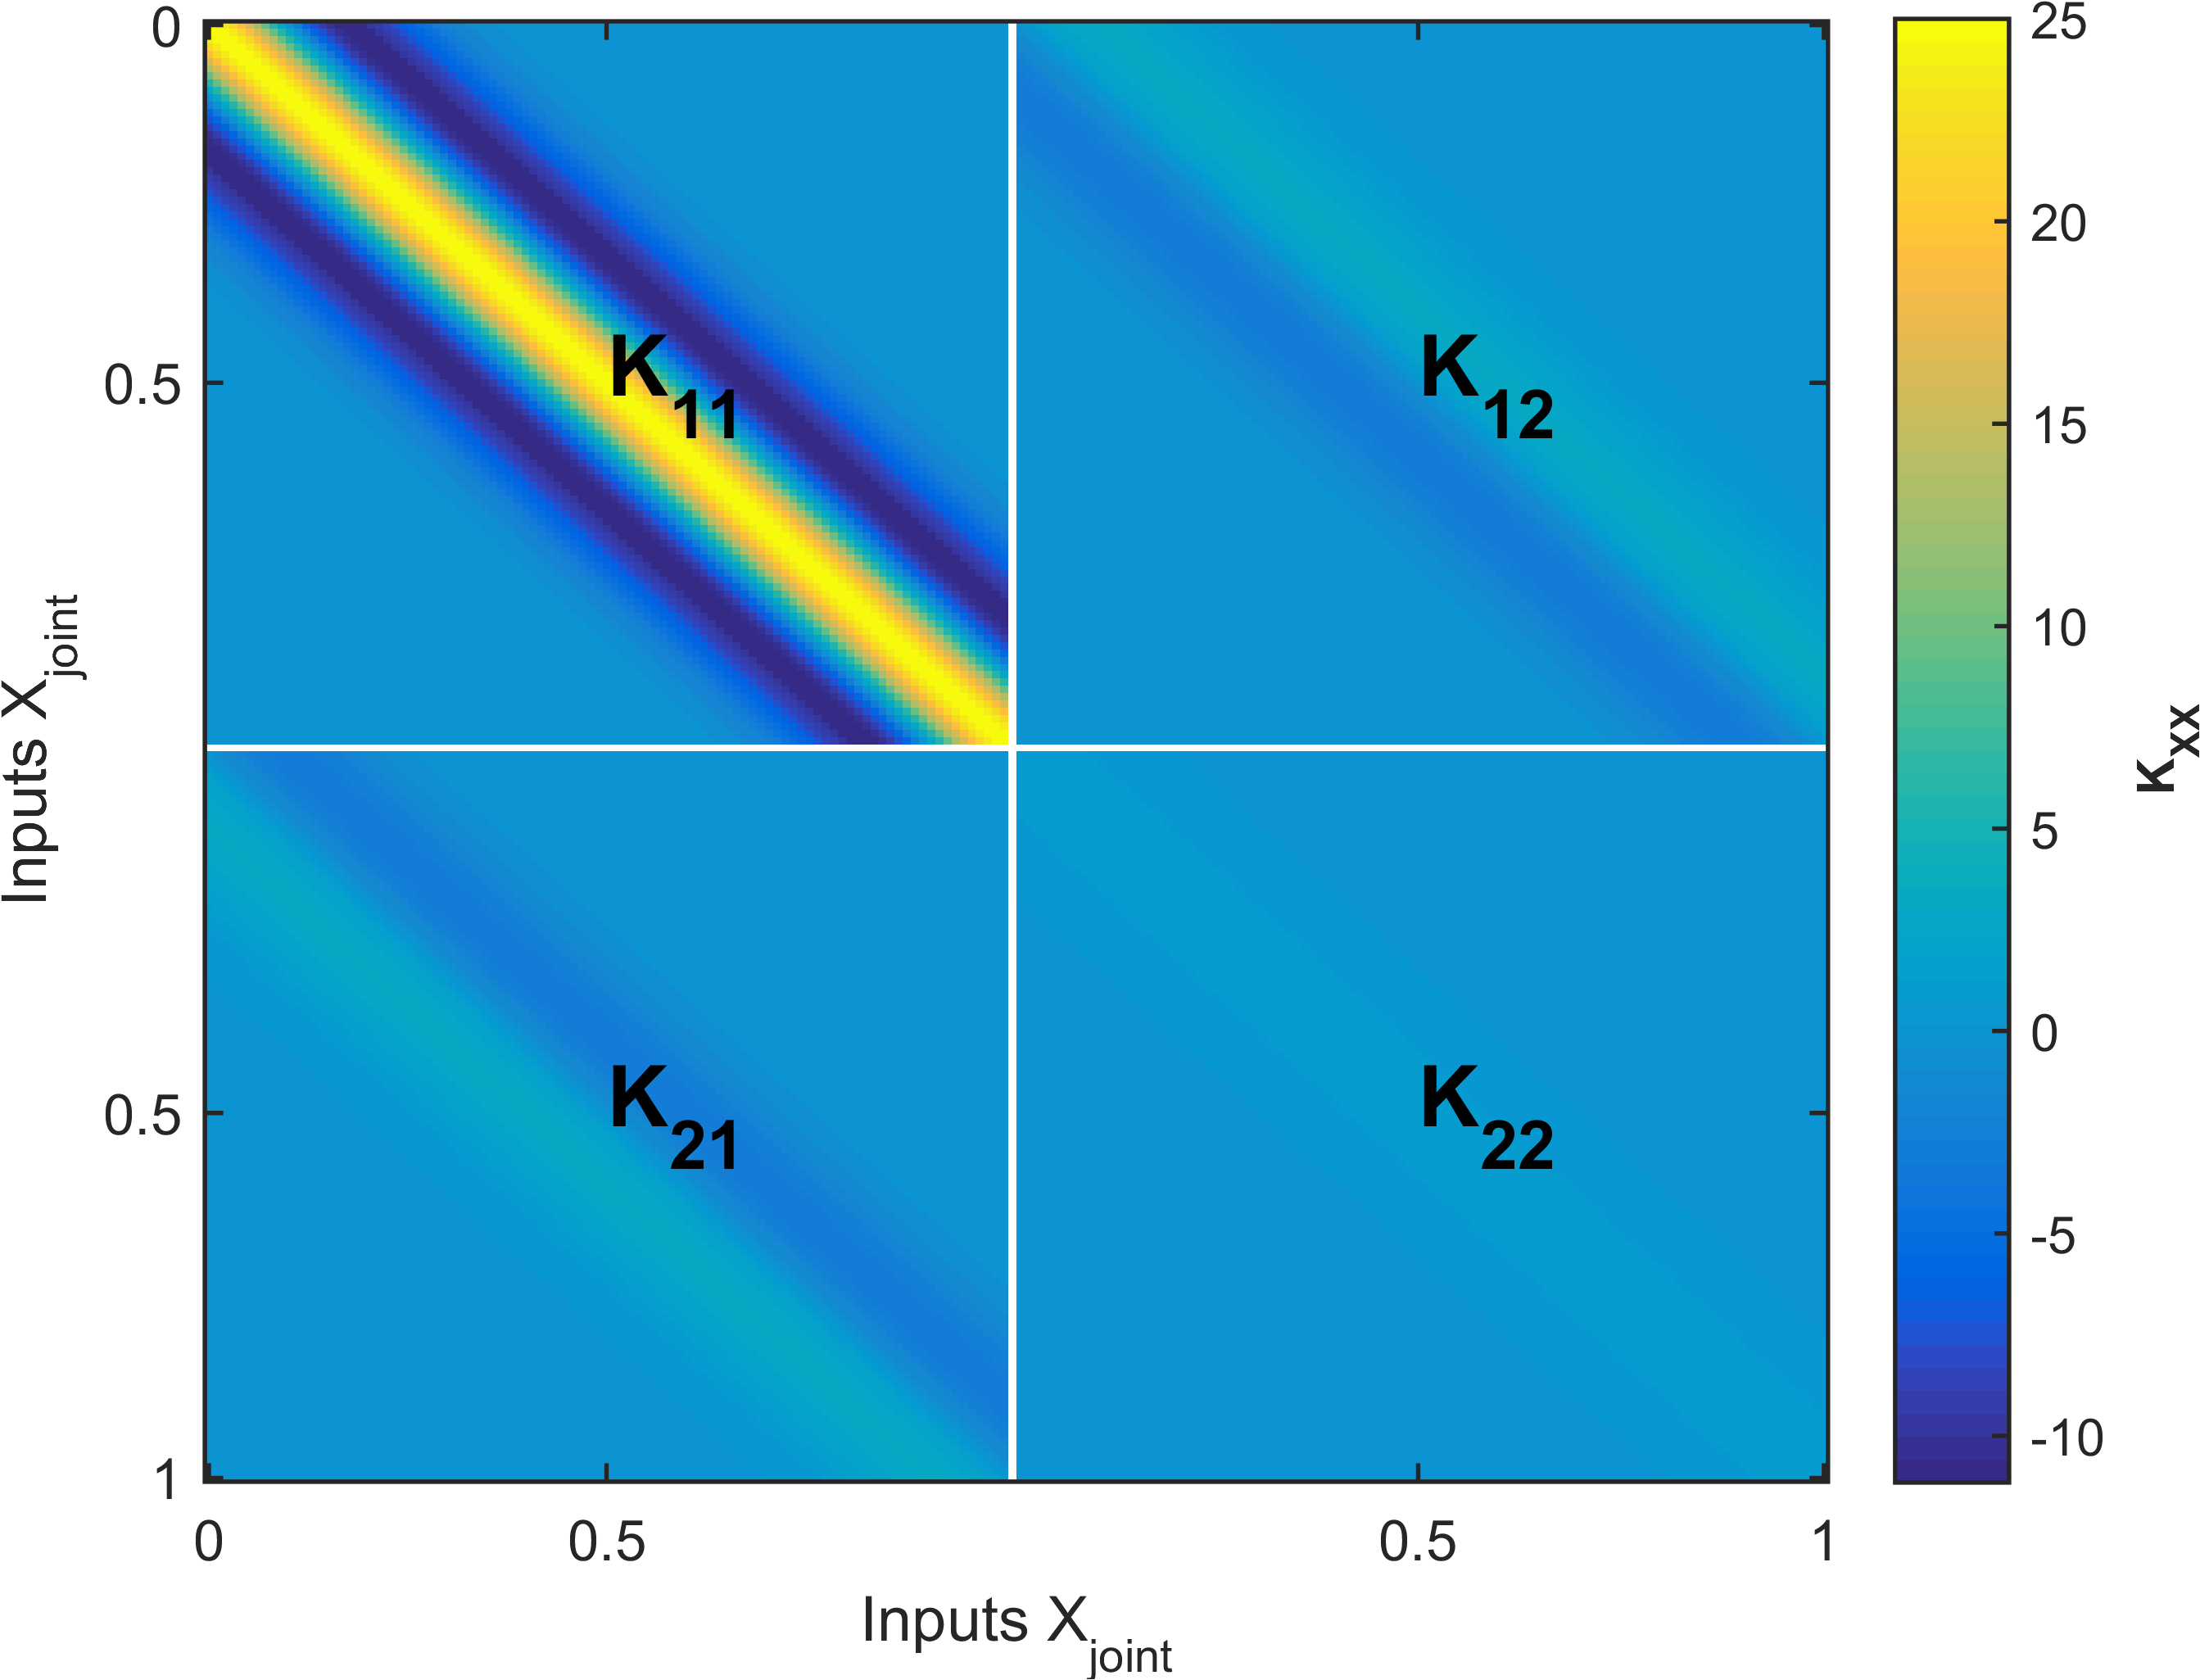
\includegraphics[width=0.45\textwidth]
  {images/part3/derivativeGramMatrix}
  \label{subfig:derivativeGramMatrix}}\quad
  \subfigure[{Gram matrix between \(y^1\) and \(y^2\) such that \(y^1 = \int_{0}^{x} y^2\). SE covariance function is used for the $y^2$ with $\theta = [1, 0.2]$, and $\myMatrix{X^j} = [0:0.01, 1]$ $\forall$ $j=[1, 2]$}]
  {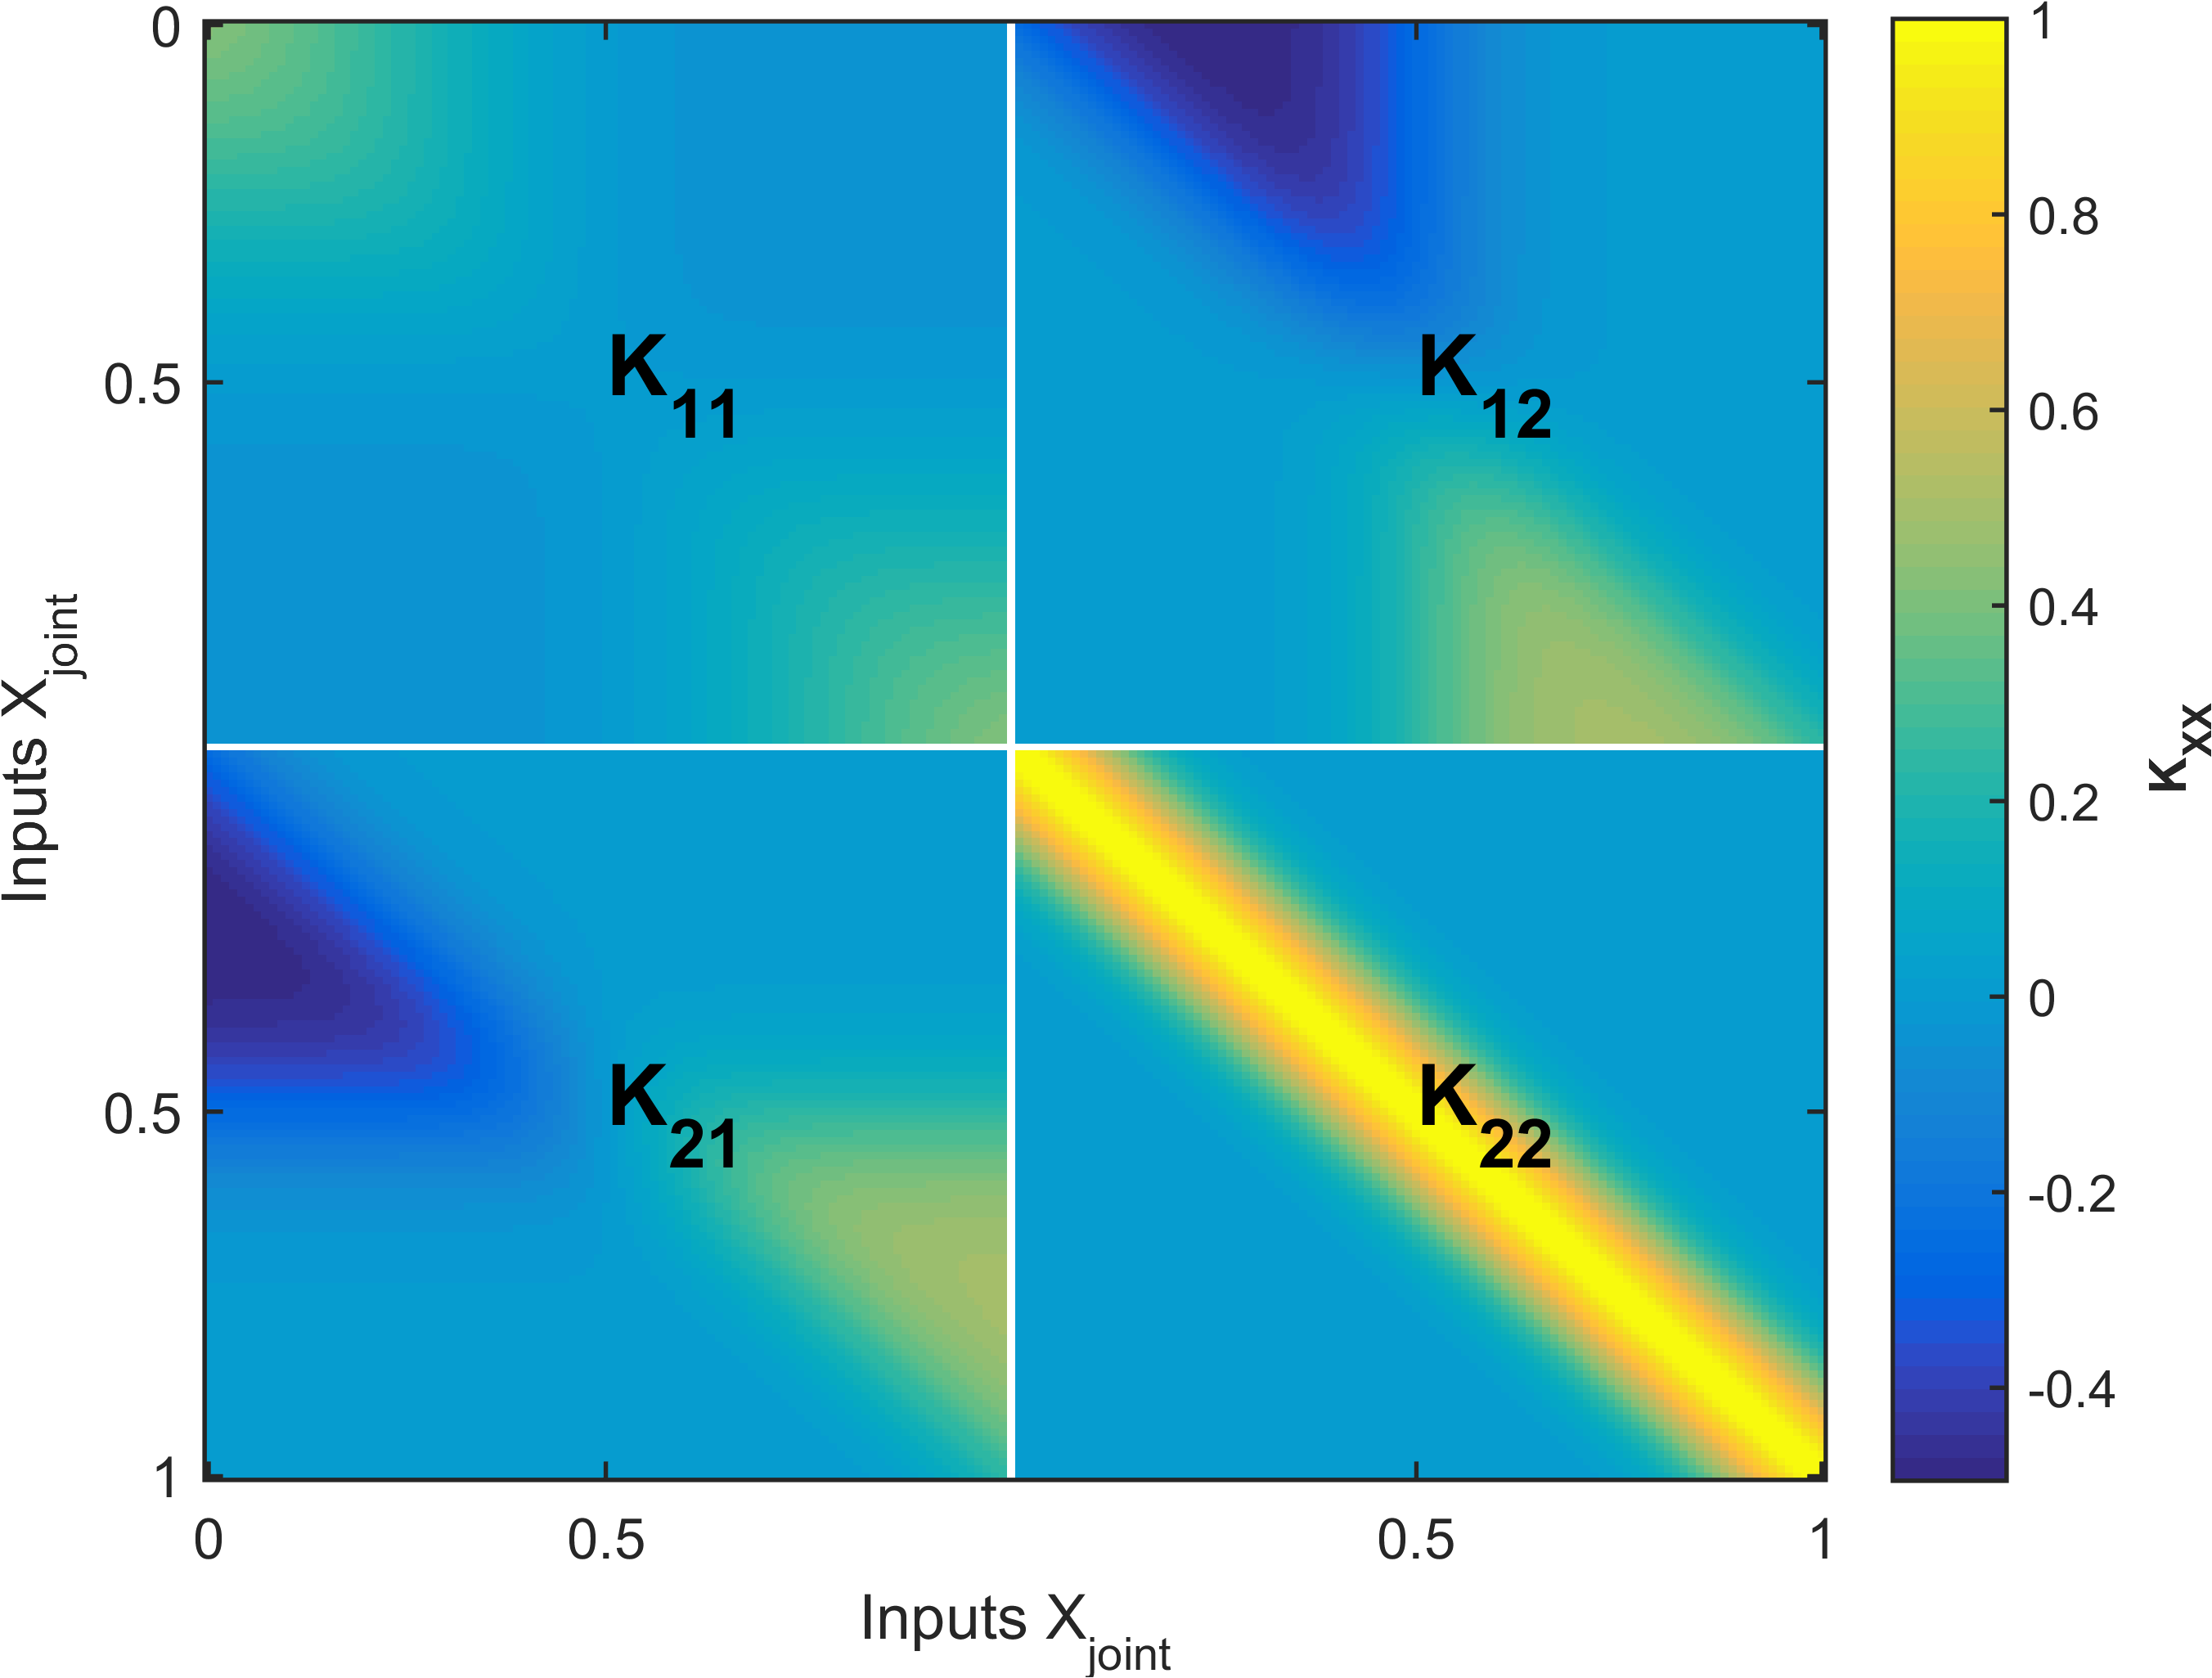
\includegraphics[width=0.45\textwidth]
  {images/part3/integralGramMatrix}
  \label{subfig:integralGramMatrix}}
  \caption{Gram matrices for the joint kernel, which encodes the relation between two outputs $y^1$ and $y^2$}
  \label{figGramMatricesJointKernel}
\end{figure}

The joint Gram matrix between \(f^{1}\) and \(f^{2}\), means that a random draw of independent function \(f^{2}\) will result in a correlated draw of the function \(f^{1}\). This effectively means that when we draw a random function \(f^{2}\) it will result in a correlated draw of \(f^{1}\), such that the two random functions will satisfy the enforced equation. 

Figure \ref{figJointRelationshipGPPriors} shows randomly drawn functions for two outputs related through an equation. The figure  \ref{subfig:drawsPriorDifferentialRelationship} shows random draws coming from a differential relationship between \(f_{differential}\) (red) and \(f_{independent}\) (blue) such that \(f_{differential} = \frac{d f_{independent}}{d x}\). We can see that the top figure is derivative of the bottom one since, \(f_{derivative}\) goes to zero where \(f_{independent}\) goes to maxima or minima. Similarly, the figure \ref{subfig:drawsPriorIntegralRelationship} shows random draws coming from an integral relationship between \(f_{integral}\) (red) and \(f_{independent}\) (blue) such that \(f_{integral} = \int_{0}^x f_{independent}\). We can see that the top figure is integral of the bottom one since, \(f_{independent}\) goes to zero where \(f_{integral}\) goes to maxima or minima. 

\begin{figure}[!ht]
  \centering
  \subfigure[{Joint draws between \(f_{differential}\) (red) and \(f_{independent}\) (blue) such that \(f_{differential} = \frac{d f_{independent}}{d x}\). We define a GP prior with zero mean and SE covariance function (\(\theta = [1, 2]\)) for the function $f^2$. }]
  {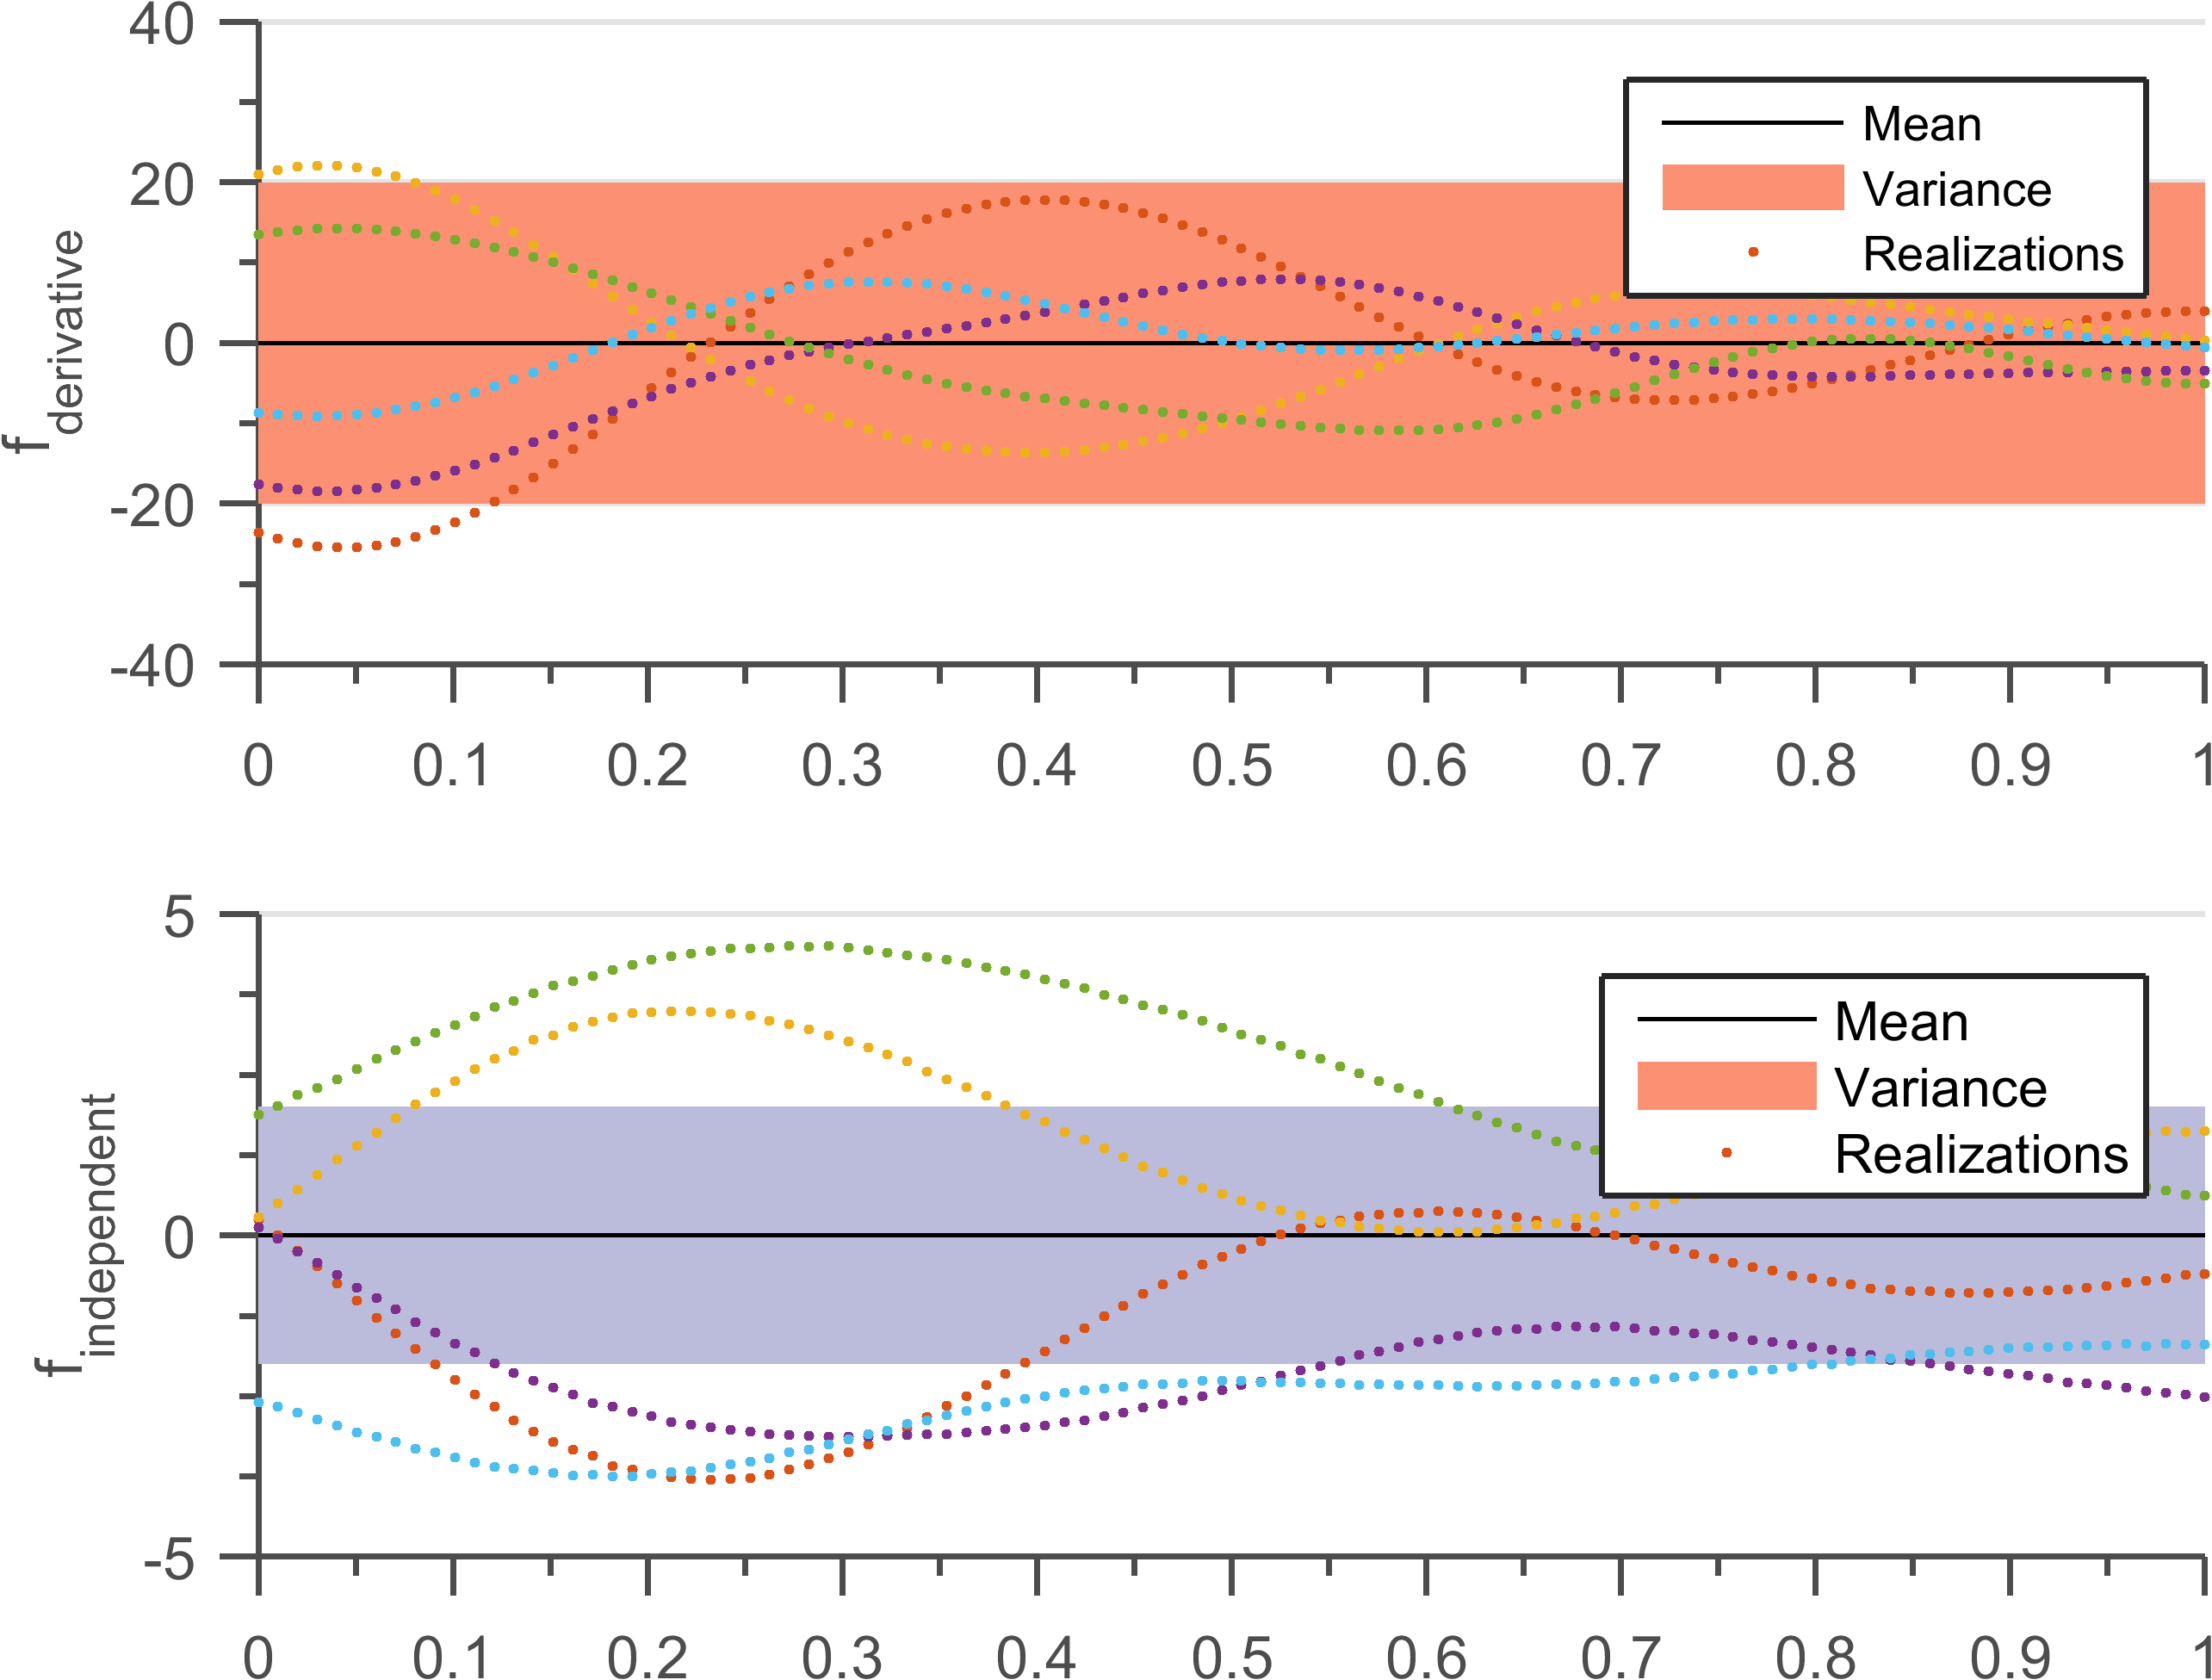
\includegraphics[width=0.485\textwidth]{images/part3/drawsPriorDifferentialRelationship}\label{subfig:drawsPriorDifferentialRelationship}}\quad
  \subfigure[{Joint draws between \(f_{integral}\) (red) and \(f_{independent}\) (blue) such that \(f_{integral} = \int_{0}^x f_{independent}\). We define a GP prior with zero mean and SE covariance function (\(\theta = [1, 2]\)) for the function $f^2$.}]
  {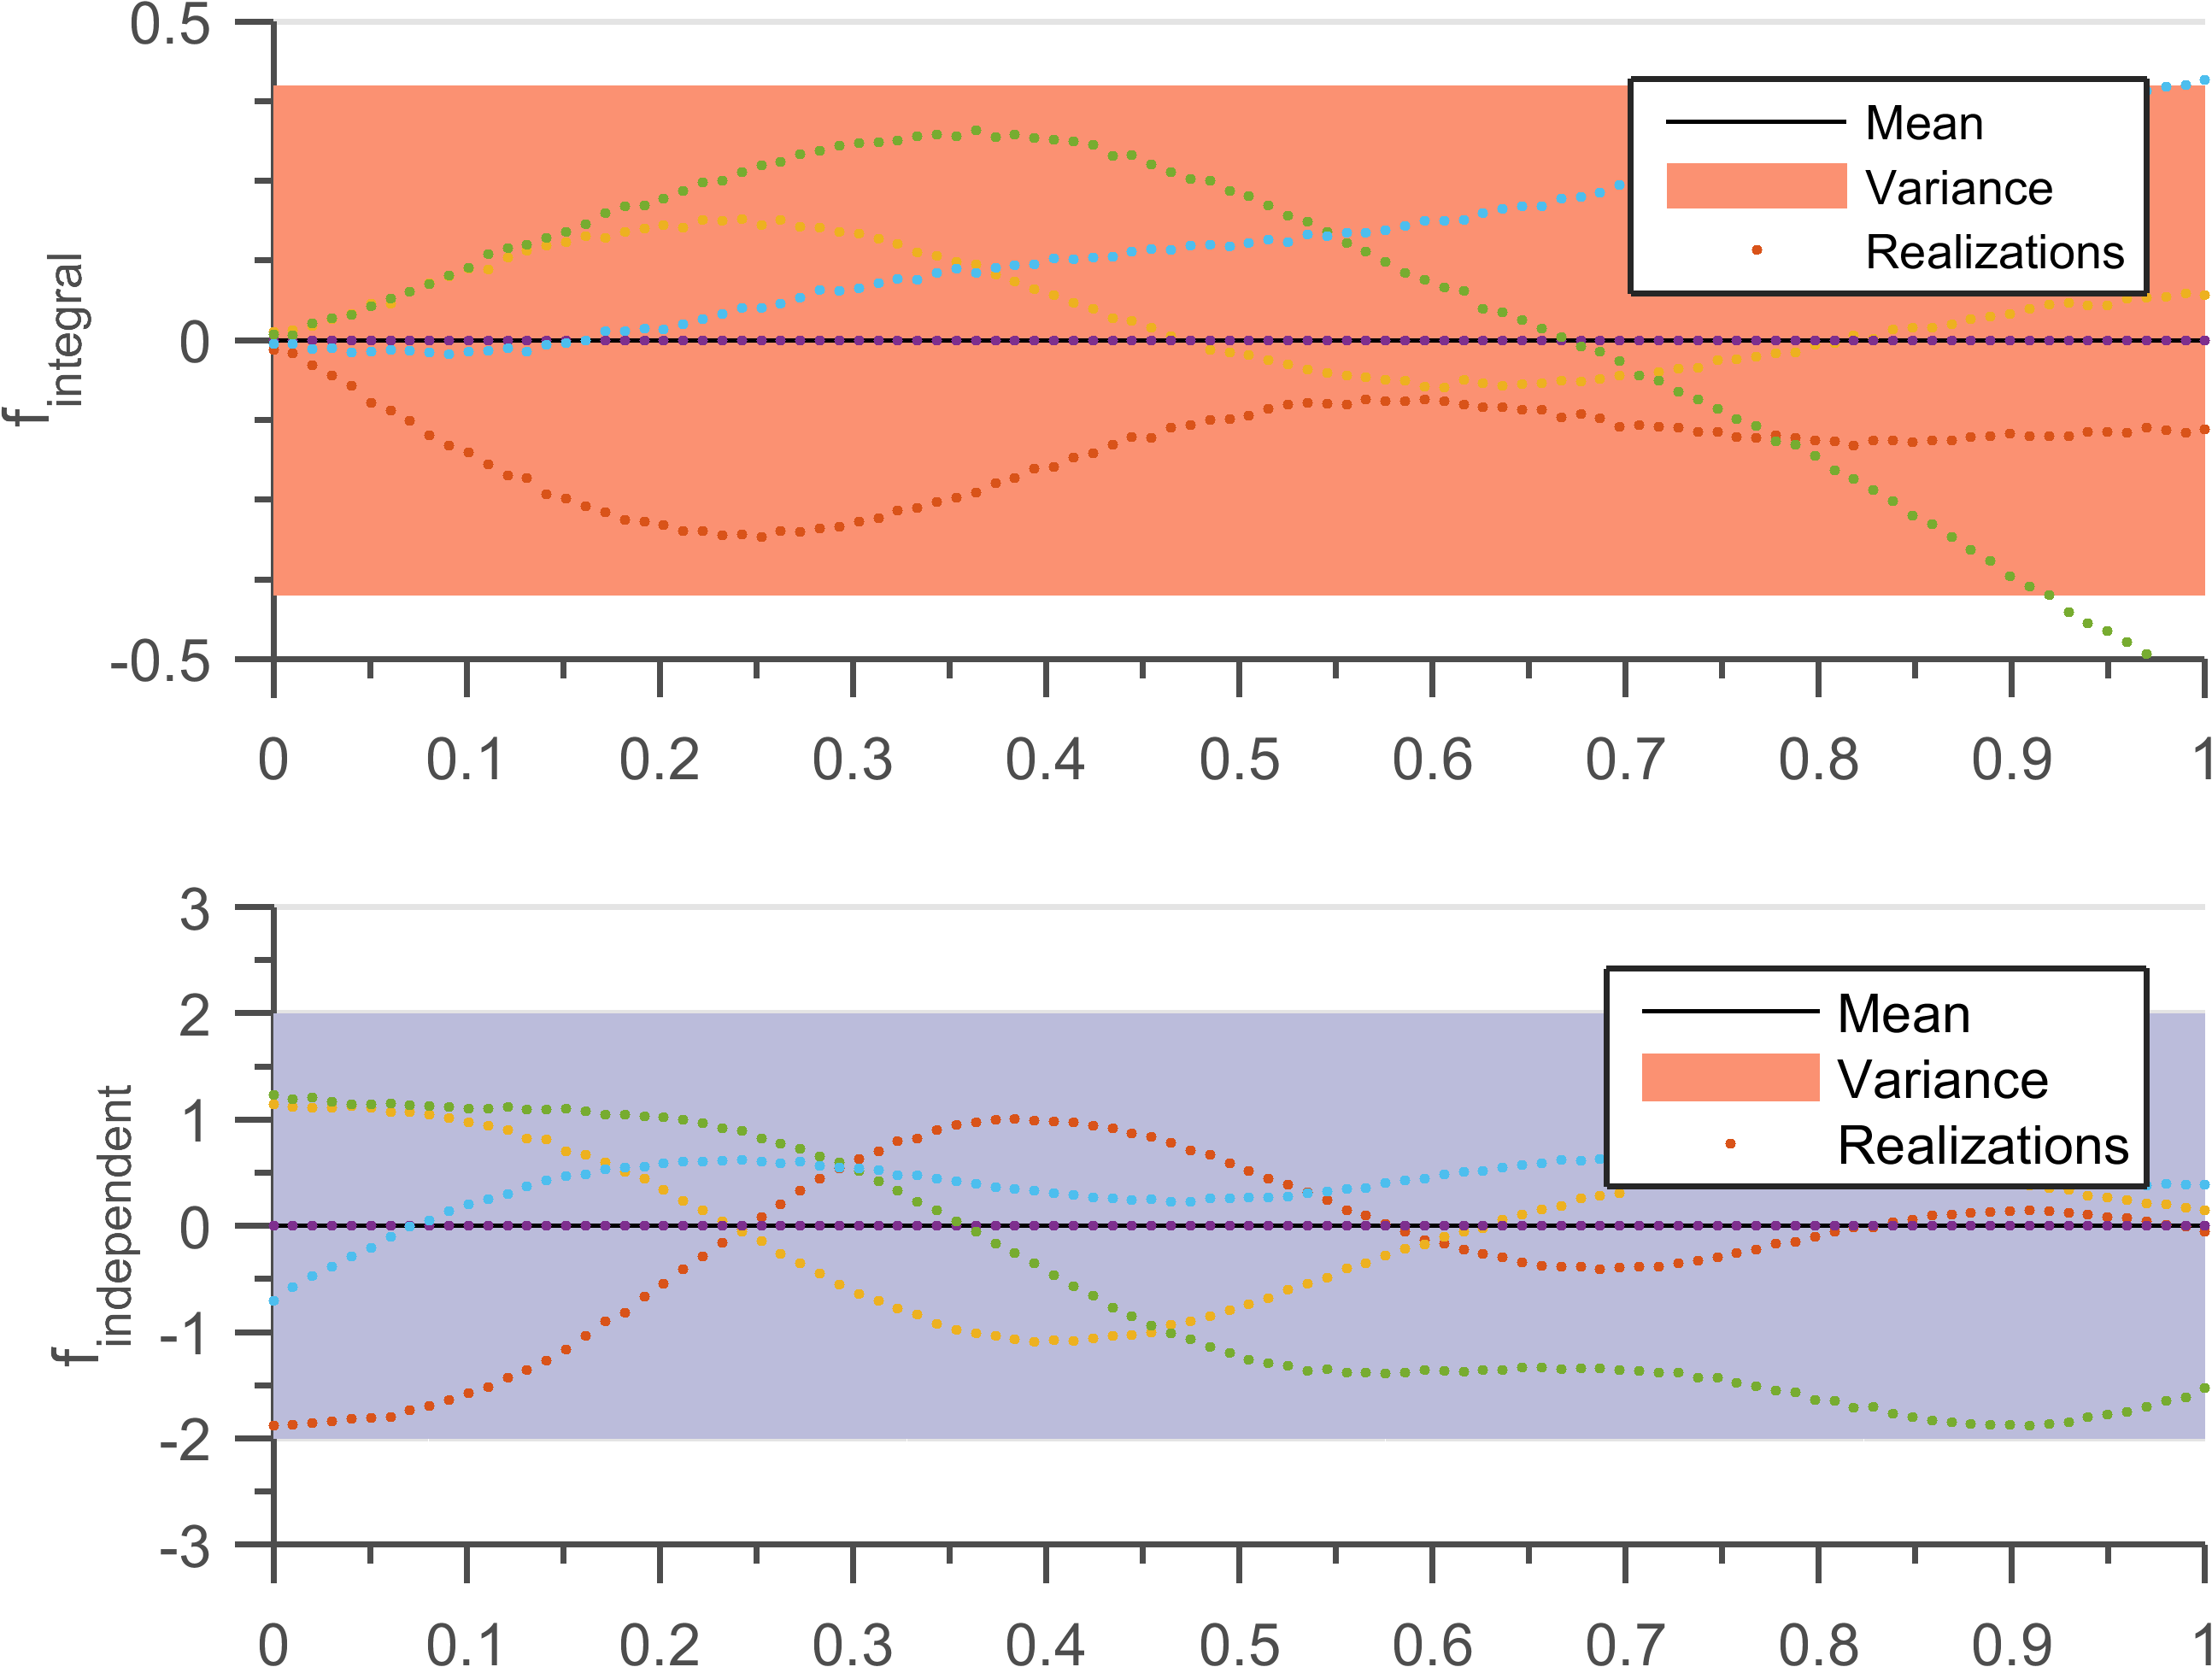
\includegraphics[width=0.485\textwidth]{images/part3/drawsPriorIntegralRelationship}\label{subfig:drawsPriorIntegralRelationship}}
  \caption{Joint draws defined by priors on related-outputs. The solid black line defines the mean function, shaded blue region defines 95\% confidence interval (2$\sigma$) distance away from the mean. The dashed lines represent five functions drawn at random from a GP prior.}
  \label{figJointRelationshipGPPriors}
\end{figure}

Proper care should be taken before performing these operations, if an operation is not defined for the prior family of functions of $f^2$, then we cannot write its corresponding joint-GP. For example, if we define a GP prior for $f^2$ with exponential covariance function (section \ref{subsecCh4MaternKernel}), we cannot enforce a differential relationship on $f^2$. This is because the exponential covariance function defines a hypothesis space of non-differentiable functions, and hence a differential operator is not-defined for such functions.  

\subsection{Case of non-linear operators}\label{subsecNonLinearOperators}
Physical laws often do not come in form of non-linear operators, but they are  difficult to solve analytically\footnote{There is a millennium prize for solving the Navier Stokes equation} for complex geometries. For example solving the structural dynamics equation is difficult for continuous complex geometries of an aircraft. One popular method to solve these differential equations is to discretize the complex geometry into simple meshes. A complex geometry of an aircraft is broken down into a simpler point, beam and plate structures, these simpler geometries are easier to solve analytically. We can then apply the physical laws on these simplistic geometries, and finally, aggregate the result of individual meshes. For example, CFD and CSM are discretized techniques to evaluate fluid and structural laws on complex geometries. These discretized operations are often non-linear and are represented in form of computer code. In this section, we wish to evaluate auto and cross-covariances across outputs related through non-linear relationships.

A non-linear operation on a GP does not result in a GP, hence for the case of non-linear \(\mathcal{L}\left ( . \right )\) the joint Gram matrix, as derived in equation \ref{eq:exactJointCovariance}, is not positive semi-definite \cite{Stein1999Springer}.  Therefore, we will use an approximate joint-covariance as developed by  \cite{Constantinescu2013} for imposing non-linear relations.

\begin{equation}\label{eq:approxJointCoariance}
K_{XX} = 
\begin{bmatrix}
L\myMatrix{K^2}L^{T} & L\myMatrix{K^2}\\ 
\myMatrix{K^2}L^{T} & \myMatrix{K^2}
\end{bmatrix} + \mathcal{O}\left ( \delta y_{2}^{3} \right )
\end{equation}

\begin{equation}
    L = \begin{matrix}
\frac{\partial \mathcal{L}}{\partial y} 
\end{matrix}|_{_{f^{2} = m^{2}}}
\end{equation}

Where $L$ is the Jacobian matrix of \(\mathcal{L}\left ( . \right )\) evaluated at the mean ($m^2$) of independent output (\(f^{2}\)). \(\delta f^{2}\) is the amplitude of small variations of \(f^{2}\), introduced by the Taylor series expansion of \(\mathcal{L}(f^2)\) with respect to \(E[f^{2}]\). 

The above covariance function takes a parametric form that depends on the mean value process of the independent variable ($E[f^2(x)]$). Equation \ref{eq:approxJointCoariance} is basically a Taylor series expansion for approximating related kernels. Since a Taylor series expansion is constructed from derivatives of a function, which are linear operations, the resulting approximated joint kernel is a Gaussian kernel with the non-Gaussian part ($\mathcal{O}\left ( \delta y_{2}^{3} \right )$) as the error. Higher-order closures can be derived with higher order derivatives of the operator \(\mathcal{L}(.)\). For simplicity we will restrict ourselves to first order approximation of the auto- and cross-covariance functions leading to an error of the order \(\mathcal{O}\left ( \delta y_{2}^{3} \right )\).  A more detailed derivation can be found at appendix \textbf{refer to link of appendix}. 

Below is a sample code (code \ref{codeNonLinearJointCovariance}) for calculating the joint-covariance functions automatically. The `jacobianOfOperator' is the jacobian of the non-linear operator $\mathcal{L}$ evaluated at the mean values of $y^2$.

\begin{mdframed}[hidealllines=true,backgroundcolor=lightgray!20]
\lstinputlisting[caption={Create joint covariance functions for non-linear operators using Matlab Symbolic Toolbox}, 
                    captionpos=b, 
                    label={codeNonLinearJointCovariance}, 
                    backgroundcolor = \color{MatlabCellColour},
                    style=Matlab-editor,
                    basicstyle=\color{black}\ttfamily\small]            {codes/chapter7/calculateNonLinearJointCovarianceFunctions.m}
\end{mdframed}

\subsection{Calculating posterior}\label{sub:MOGPs}
The posterior distribution can be calculated by conditioning the prior distribution on the observation dataset. Since a prior distribution over functions defined over the joint dataset is also a GP, we can easily derive the posterior mean, posterior covariance and marginal likelihood (the exact derivations are described in section \ref{subsecPosteriorDistribution}). We just need to insert the appropriate Gram matrix ($\myMatrix{K_{XX}}$) in the equations of posterior mean (equation \ref{eq:predictiveMOMeanCh7}), posterior variance (equation \ref{eq:predictiveMOCovarianceCh7}) and marginal likelihood (equation \ref{eq:exactMONLMLCh7}). 

\begin{align}
  E[f(X_{*}))] & = K_{X_{*}X}\left ( K_{XX} + \Sigma \right )^{-1}\VEC{y_{joint}} \label{eq:predictiveMOMeanCh7} \\ 
  Cov(f(X_{*})) & = K_{X_{*}X_{*}} - K_{X_{*}X}\left ( K_{XX} + \Sigma \right )^{-1}K_{XX_{*}} \label{eq:predictiveMOCovarianceCh7} \\
  \log(\Pr[\VEC{y_{joint}} \mid X, \theta]) & = \log[GP(\VEC{y_{joint}}| 0, K_{XX} + \Sigma )] \label{eq:exactMONLMLCh7}
\end{align}

\paragraph{Example}
The figure \ref{subfig:drawsDifferentialRelationship} shows mean and variance for a differential relationship between independent function \(f_{independent}\) (blue) and differential function \(f_{derivative}\) (red), such that \(f_{derivative} = \frac{\partial f_{independent}}{\partial x}\). We have conditioned the two functions such that \(f_{derivative}|_{x = 0} = 5\) and \(f_{independent}|_{x = 0} = 0\). This means that the function \(f_{independent}\) passes through \(0\) and has a derivative equal to \(5\) at \(x = 0\). It is easy to observe that all the functions of \(f_{independent}\) that pass through $x=0$ have the same value of derivatives.
We have not maximized the marginal likelihood for this case and the hyperparameters of \(k^2\) are \(\theta_{amplitude} = 1; \theta_{lengthScale} = 0.2\). 

Figure \ref{subfig:drawsIntegralRelationship} shows mean and variance for an integral relationship between independent function \(f_{independent}\) (blue) and differential function \(f_{integral}\) (red) and such that \(f_{integral} = \int_0^x f_{independent}z . dz\). We have conditioned the two functions such that \(f_{integral}|_{x = 1} = 0\) and \(f_{integral}|_{x = 0} = 0\). This means that the function \(f_{independent}\) has an integral \(0\) at the two points \([0, 1]\) . Although it is difficult to verify from the figure, but all the randomly drawn functions of \(f_{independent}\) indeed have their integral ($\int_{0}^{1} f_{independent} = 0 $) equal to zero. We have not maximized the marginal likelihood for this case and the hyperparameters of \(k^2\) are \(\theta_{amplitude} = 1; \theta_{lengthScale} = 0.2\). All the corresponding draws from the posterior GP also follow the conditioning. 

\begin{figure}[!ht]
  \centering
  \subfigure[Joint draws between \(f_{derivative}\) \(red\) and \(f_{independent}\) \(blue\) such that \(f_{derivative} = \frac{\partial f_{independent}}{\partial x}\). The posterior is conditioned such that \(f_{derivative}|_{x = 0} = 5\) and \(f_{independent}|_{x = 0} = 0\). The draws from the posterior follow the relationship between outputs and also the conditioning.]
  {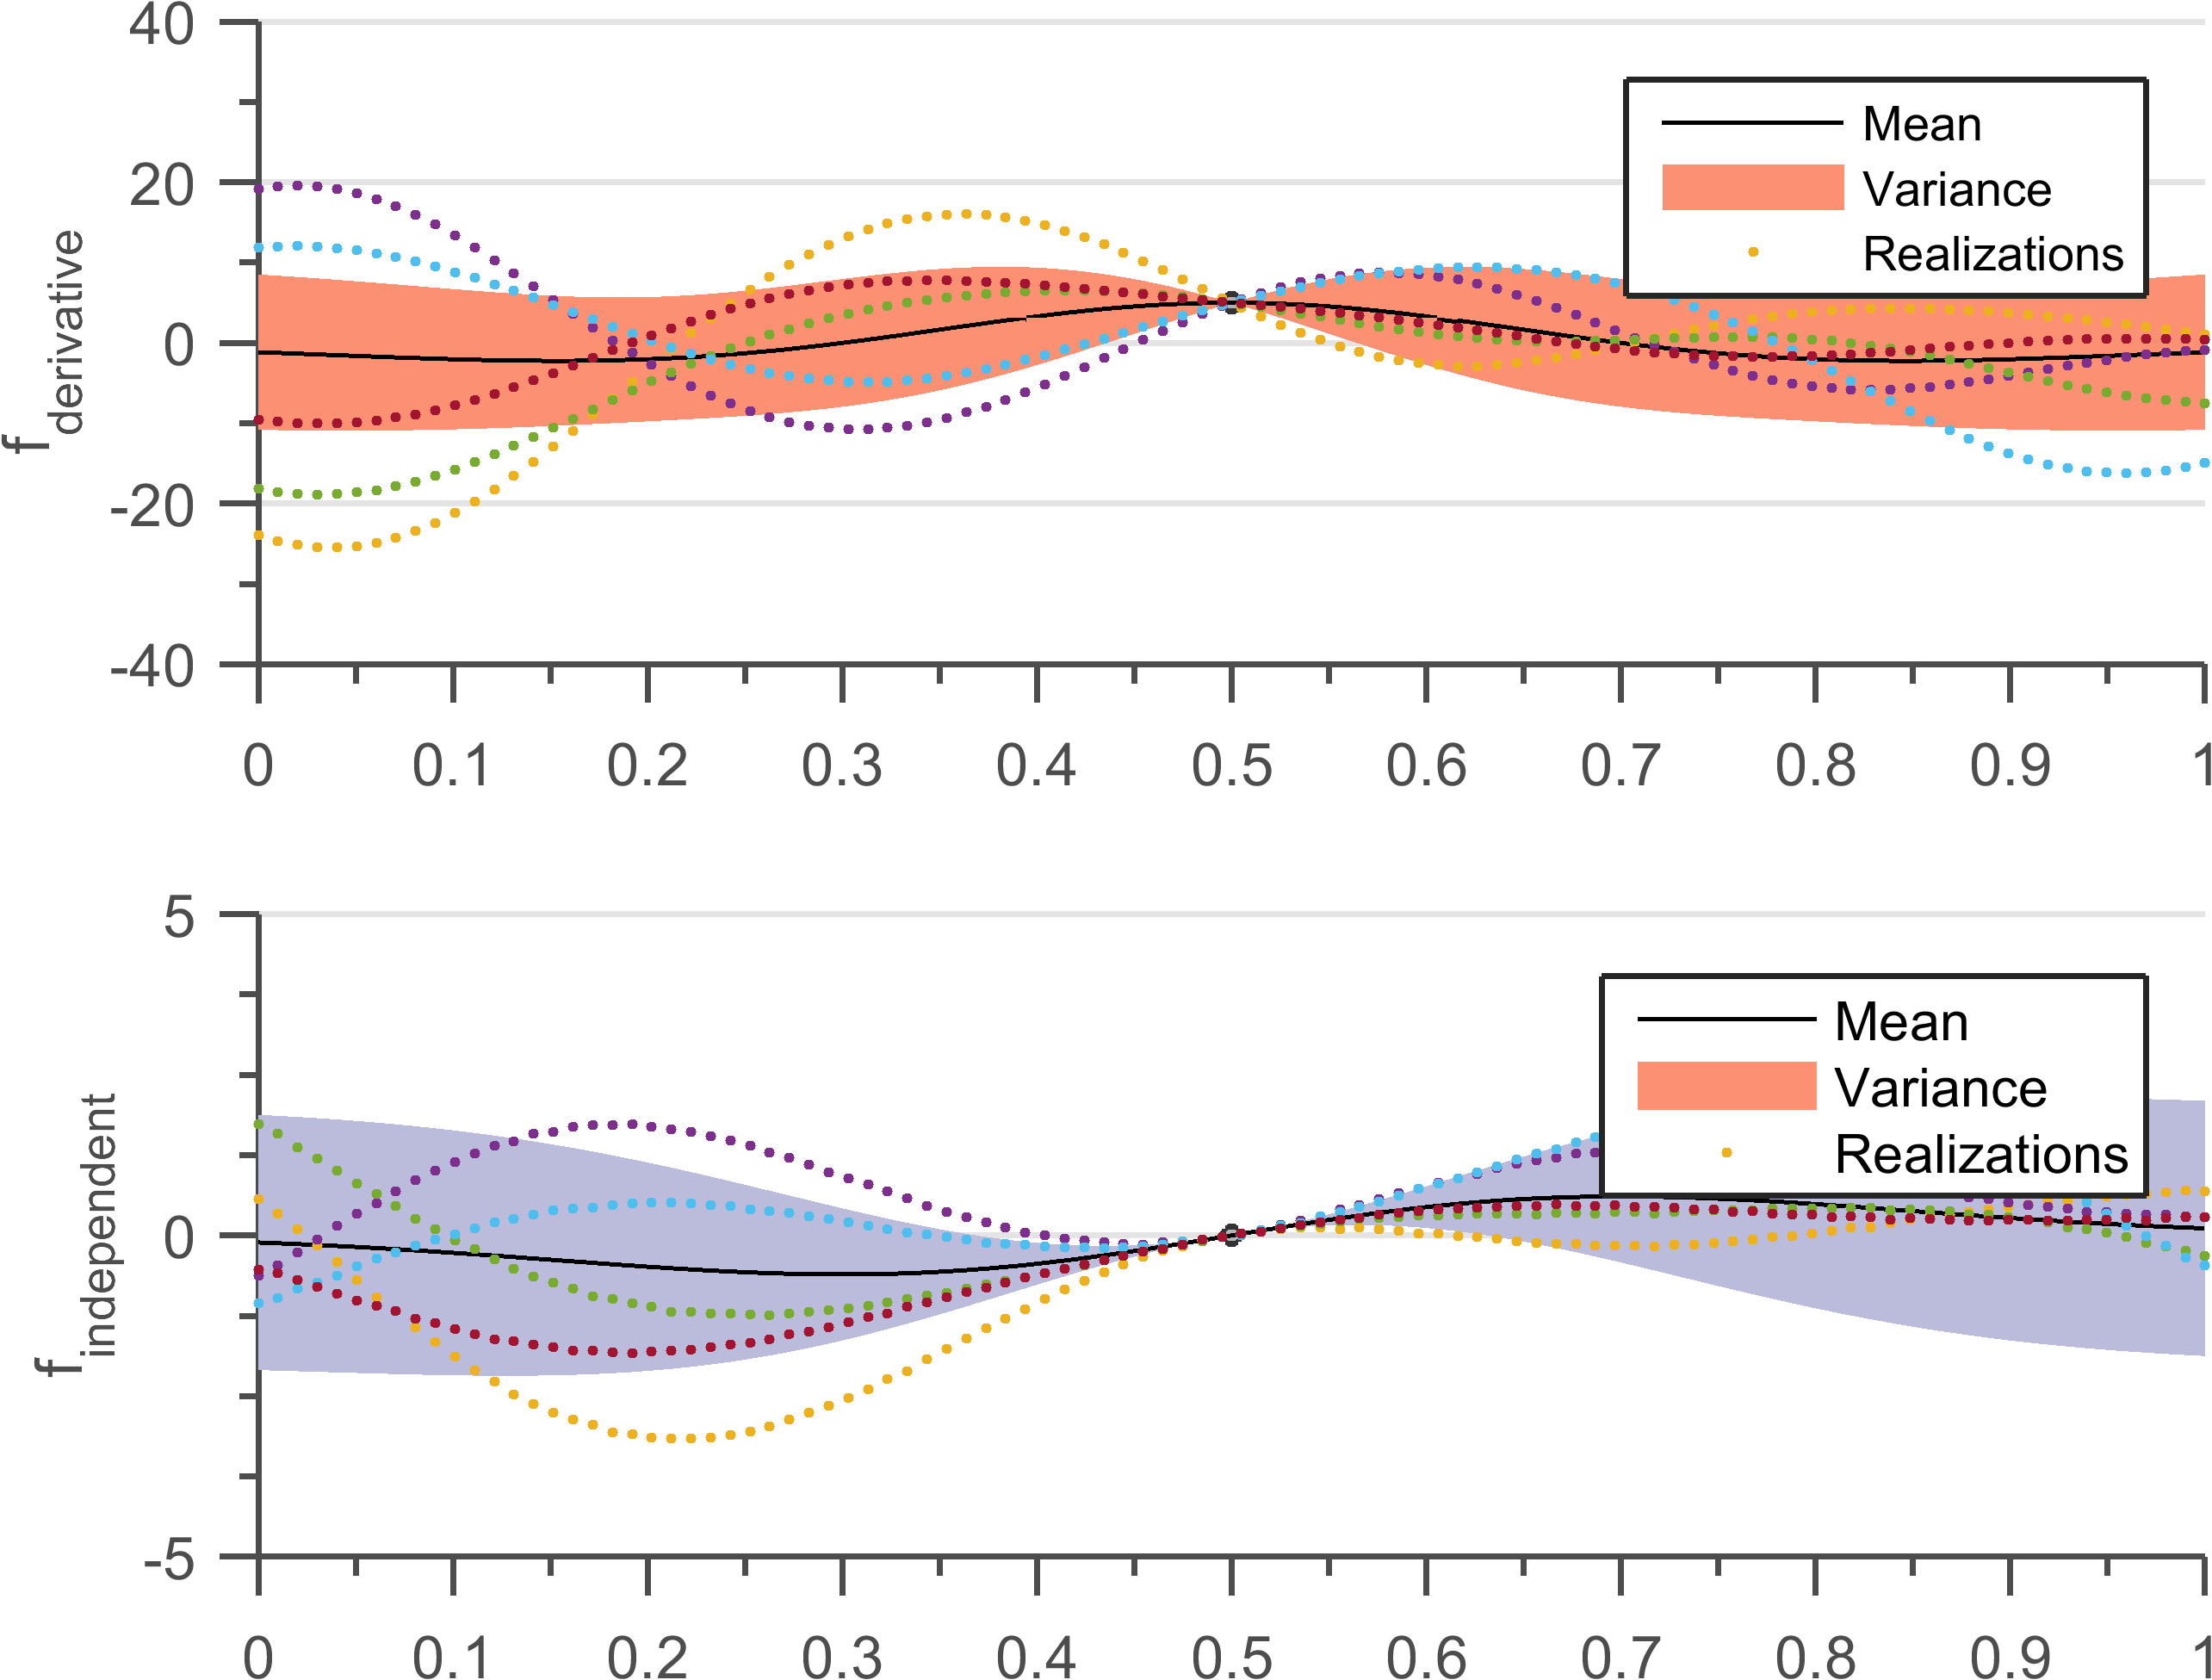
\includegraphics[width=0.485\textwidth]{images/part3/drawsDifferentialRelationship}\label{subfig:drawsDifferentialRelationship}}\quad
  \subfigure[Joint draws between \(f_{integral}\) \(red\) and \(f_{independent}\) \(blue\) such that \(f_{integral} = \int f_{independent}\). The posterior is conditioned such that \(f_{integral}|_{x = 0} = 0\) and \(f_{integral}|_{x = 1} = 0\). The draws from the posterior follow the relationship between outputs and also the conditioning.]
  {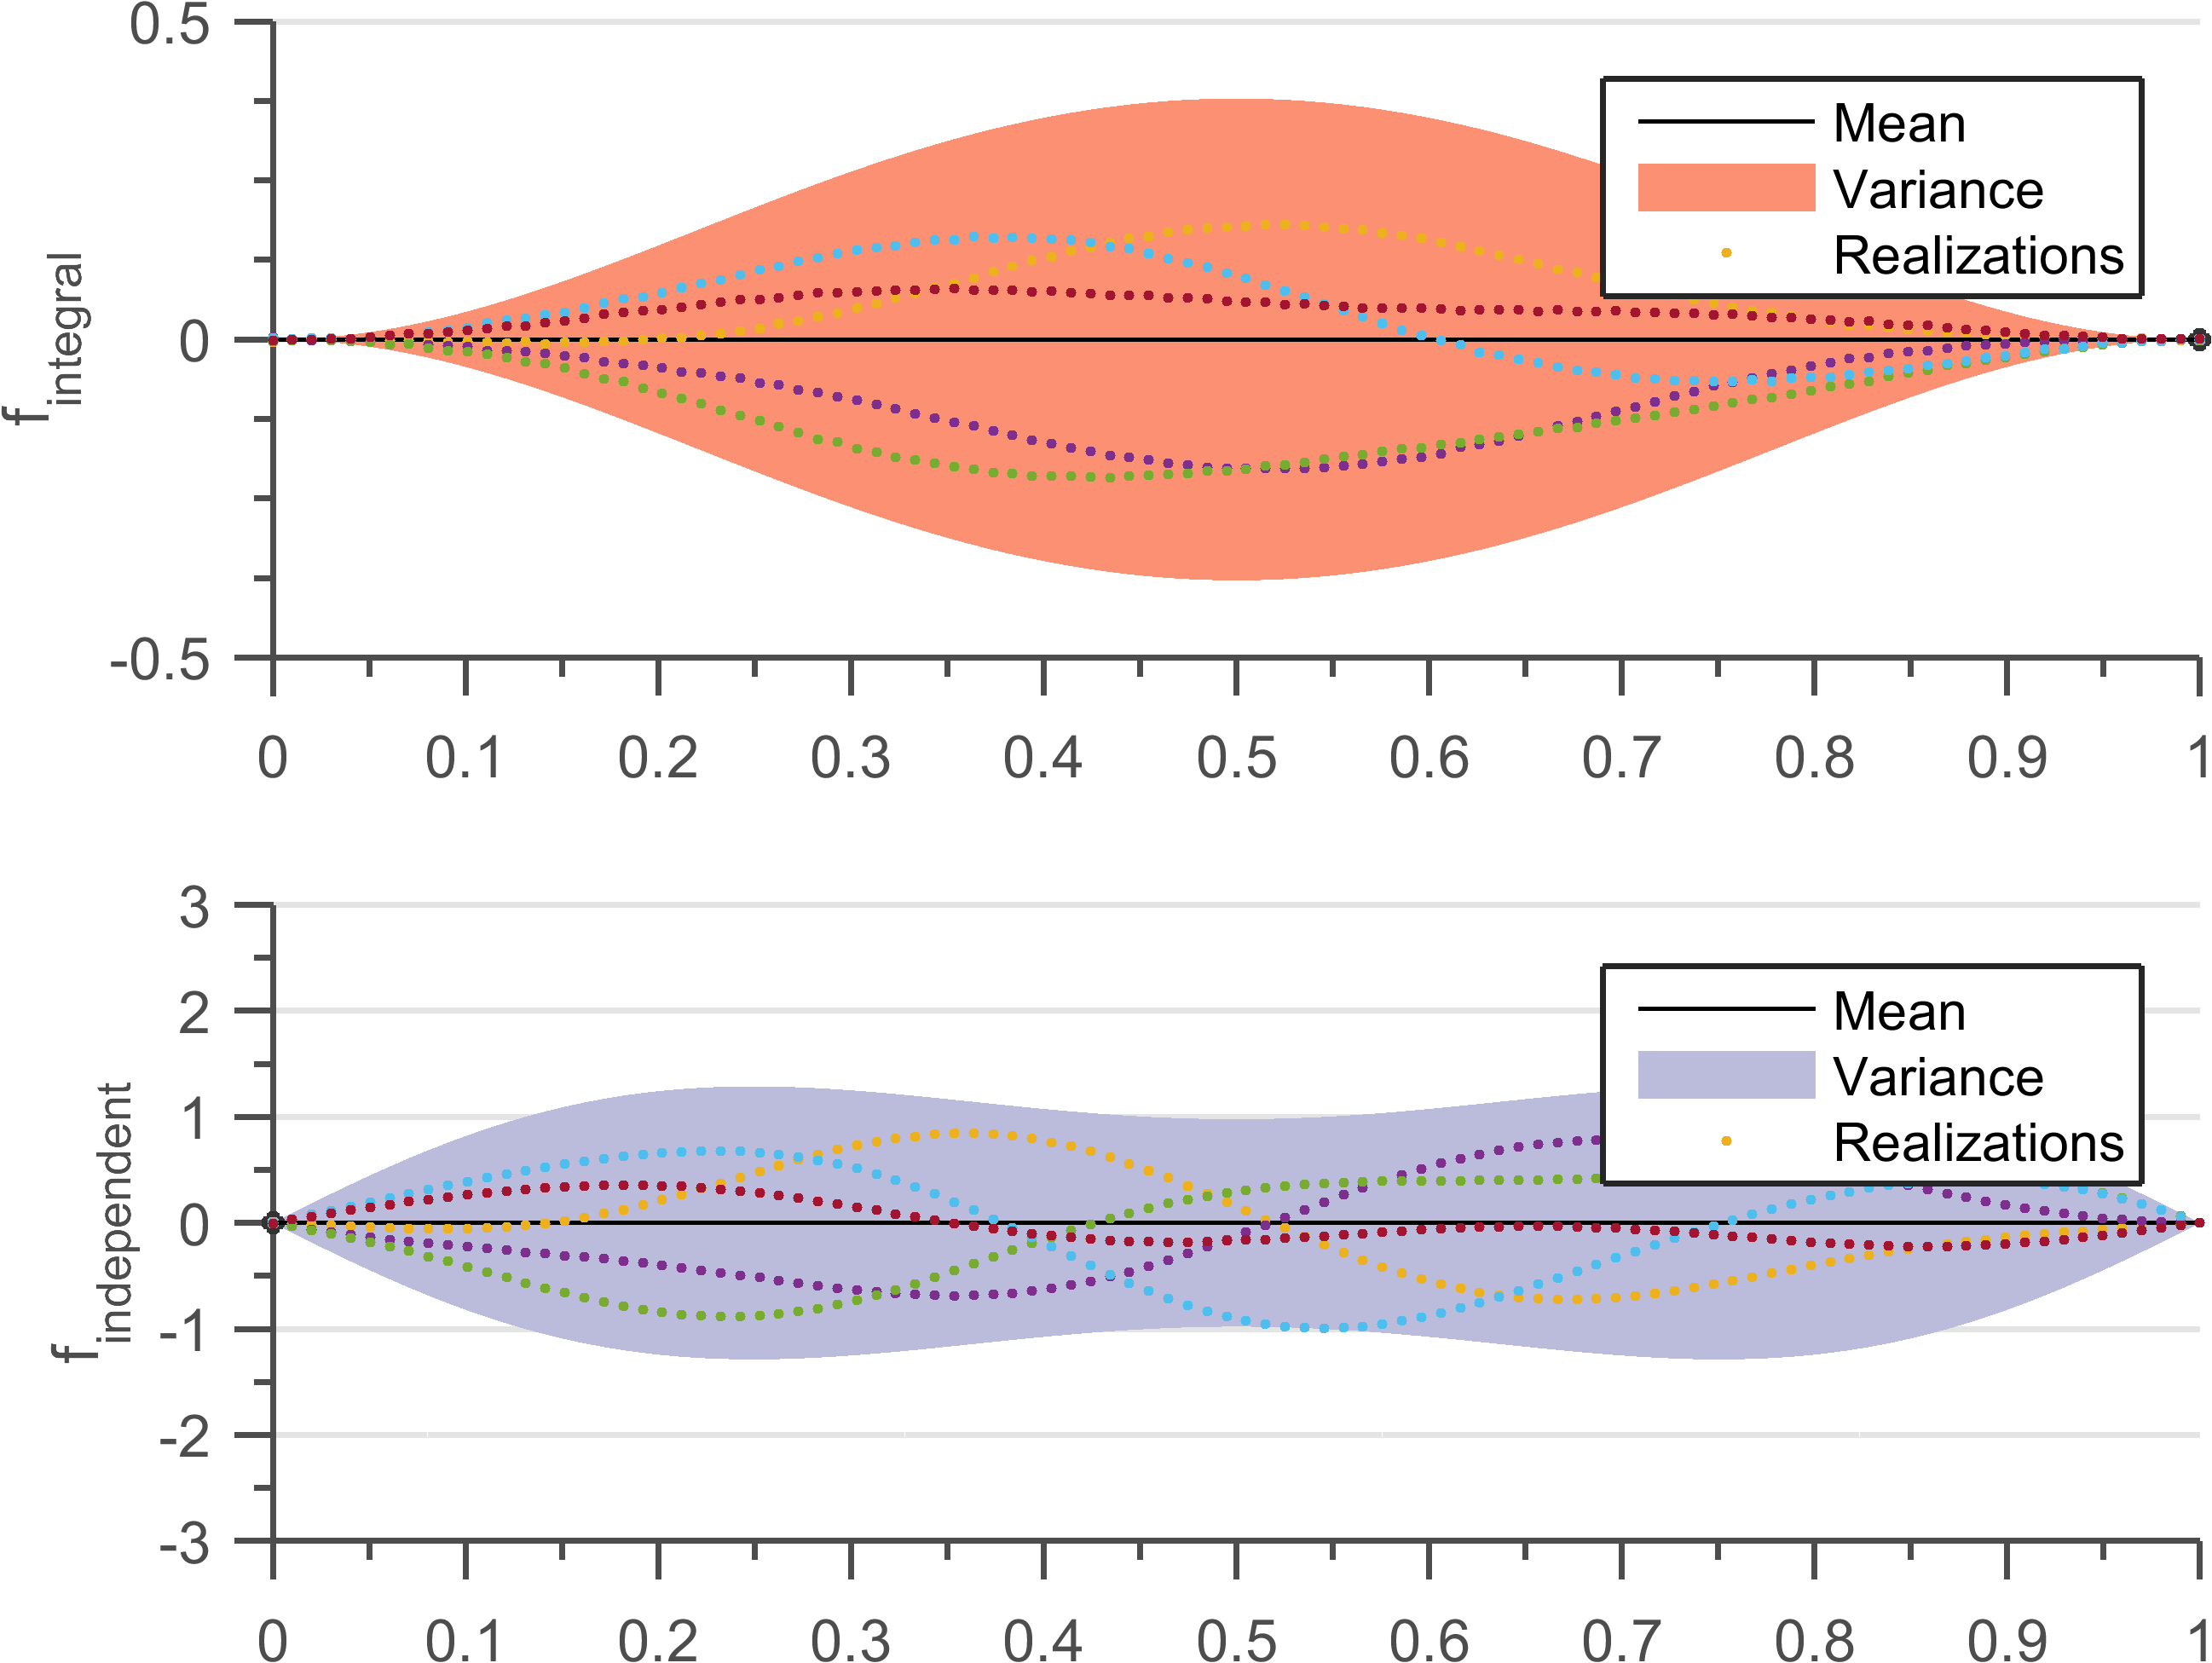
\includegraphics[width=0.485\textwidth]{images/part3/drawsIntegralRelationship}\label{subfig:drawsIntegralRelationship}}
  \caption{Multi-Output Gaussian Process Regression Predictions. The solid black line defines the mean function, shaded region defines 95\% confidence interval (2$\sigma$) distance away from the mean. Dotted lines represent the functions randomly drawn from the posterior distributions.}
\end{figure}

In the next section, we compare the prediction capabilities of independent GP, with that of multi-fidelity GP and joint relationship enforced GP on a synthetic dataset. We then take a real flight-test dataset and study the effects of different prior $k^2$ on their predictions.

\section{Experiments}\label{sec:results}
In this section, we provide a numerical illustration to the theoretical derivations in the earlier sections. We start with a synthetic problem where we try to learn the model over quadratic relationships. We compare the cross-validation error values of independent GP regression with that of multi-fidelity GP and relationship enforced joint MTGP. Finally, we study the effect of choosing different prior for the independent function $f^2$ on a dataset for flight-loads estimation for the horizontal tail plane.

The basic toolbox used for this section is GPML provided with \cite{Rasmussen2005}, we generate covariance functions to handle relationships as described in equations \ref{eq:exactJointCovariance} using the ``Symbolic Math Toolbox" in MATLAB 2014b (code \ref{codeJointCovariance} and \ref{codeNonLinearJointCovariance}). 

\subsection{Quadratic relation on Synthetic Data}\label{sub:experimentsSyntheticData}
We take the case of a quadratic operator \(\mathcal{L}(.)\) equation \ref{eq:quadraticRelationship}. 
\begin{equation}\label{eq:quadraticRelationship}
f^{1} = \left [f^{2} \right]^2
\end{equation}

To generate the data, we randomly draw a single function of \(f^{2}\) as described in equation \ref{eq:experimentalSET} for 50 equally spaced inputs between [-1, 1]. The output \(f^{1}\) is then calculated by applying the operation in equation \ref{eq:quadraticRelationship}. The latent functions \(f's\) are then corrupted according to equation \ref{eq:experimentalSET} which gives us the outputs \(y's\). We finally hide the observations for \(y^{1}\) in the domain \(x = [-0.2, 0.2]\). We now have our dataset for testing the performance of quadratic relationship. 

\begin{equation}\label{eq:experimentalSET}
\begin{aligned}
\Pr[f^{2}] & =   GP[0, K_{SE}(0.2, 1)] \\
\Pr[\sigma_{n2}] & = \mathcal{N}[0, 0.1] \\
\Pr[\sigma_{n1}] & = \mathcal{N}[0, 1]
\end{aligned}
\end{equation}
     
\(K_{SE}(1, 0.2)\) means squared exponential kernel with length scale 0.2 and variance as 1. \(\sigma_{n2}\) and \(\sigma_{n1}\) are the white noises added to the latent functions \(f^{1}\) and \(f^{2}\) respectively. Since the quadratic relationship \(\mathcal{L}(.)\) is non-linear in nature we use equation \ref{eq:approxJointCoariance} to calculate the auto- and cross-covariance functions as shown in equation \ref{eq:jointKernelForQuadratic relationship}. 

\begin{equation}\label{eq:jointKernelForQuadratic relationship}
    \begin{aligned}
Cov(f^2(x), f^2(x')) & = k^{2} \\    
Cov(f^1(x), f^2(x')) & = 2m^{2}(x^{1}) k^{2} \\
Cov(f^1(x), f^1(x')) & = 4 \left [m^{2}(x^{1}) \right ]^2 k^{2}
    \end{aligned}
\end{equation}

Here, \(m^2(x^{1})\) is the mean value of function \(y^{2}\) calculated at the input points \(x^{1}\). For the case of quadratic relationship the Jacobian \(L\) as described in equation \ref{eq:approxJointCoariance} comes out to be \(2*\mu_{y^{2}}(x)\). For non-linear operators \(\mathcal{L}(.)\) the joint-covariance prior depends on the mean value of \(f^{2}\) ($\mu_{y^{2}}$). \(Cov(f^1(x), f^1(x'))\) and \(Cov(f^1(x), f^2(x'))\) are the covariance functions calculated at the input points \(x\) and \(x'\) as described in equation \ref{eq:approxJointCoariance} and equation \ref{eq:mogpJointPrior}. We can observe that the joint-covariance has been expressed as a function of covariance \(k^2\) using equation \ref{eq:quadraticRelationship}.  


Figure \ref{subfigquadraticRelationshipIndependent} shows the independent fit of two GP regressions. For the case of \(y^{1}\), there is a huge difference between the real data and predicted mean at points where data is unavailable. Figure \ref{subfigquadraticRelationshipMultiFidelityKernel} shows the fit using multi-fidelity GP regression model (section \ref{secMultiFidelityMTGP}). We can observe that the multi-fidelity model cannot capture the quadratic nature of the relationship between outputs. Figure \ref{subfigquadraticRelationshipJointKernel} shows the joint-GP regression, which gives better prediction even in the absence of data for \(y^{1}\) because a transfer of information is happening from observations of \(y^{2}\) present at those locations. 

\begin{figure}[!ht]
  \centering
  \subfigure[{Independent GP Regression for the two outputs \(y^{1}\) and \(y^{2}\). We can observe the huge difference between the real data and the predicted mean values at zone with no data.}]
  {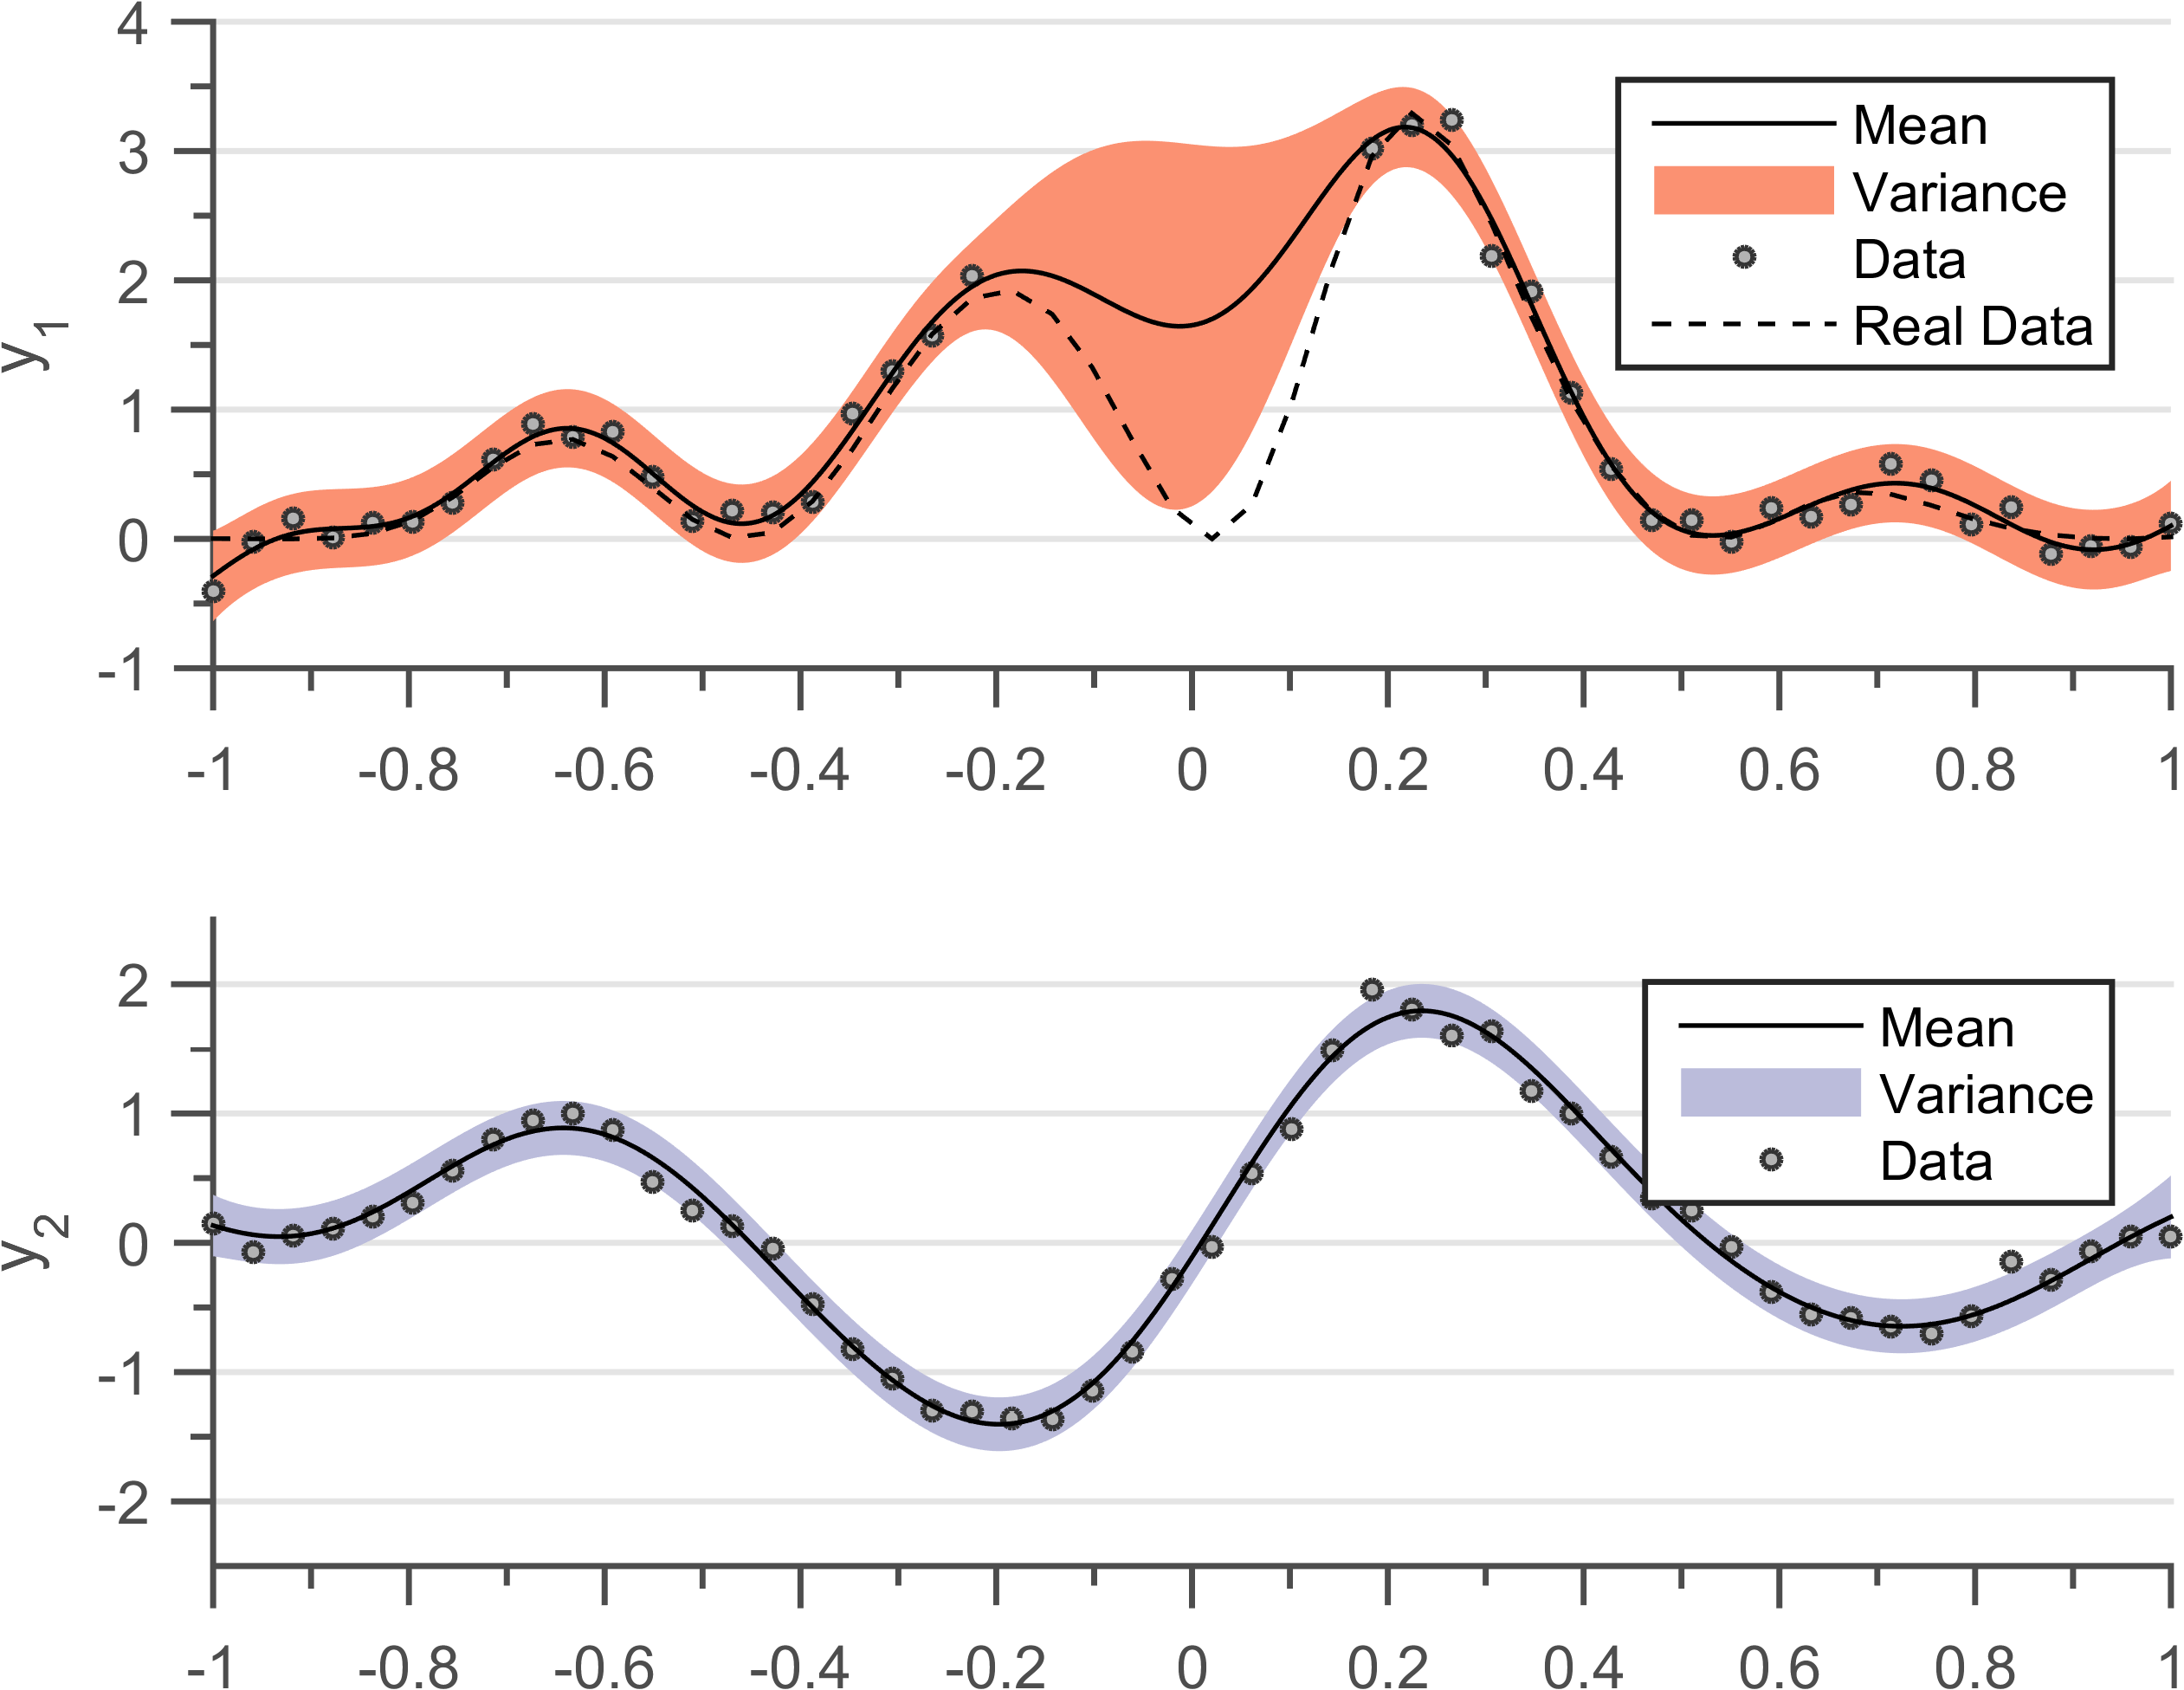
\includegraphics[width=0.3\textwidth]
  {images/part3/quadraticRelationshipIndependent}
  \label{subfigquadraticRelationshipIndependent}}
  \quad
  \subfigure[{Multi-fidelity GP Regression for the two outputs \(y^{1}\) and \(y^{2}\) (section \ref{secMultiFidelityMTGP}). We can observe the huge difference between the real data and the predicted mean values at zone with no data.}]
  {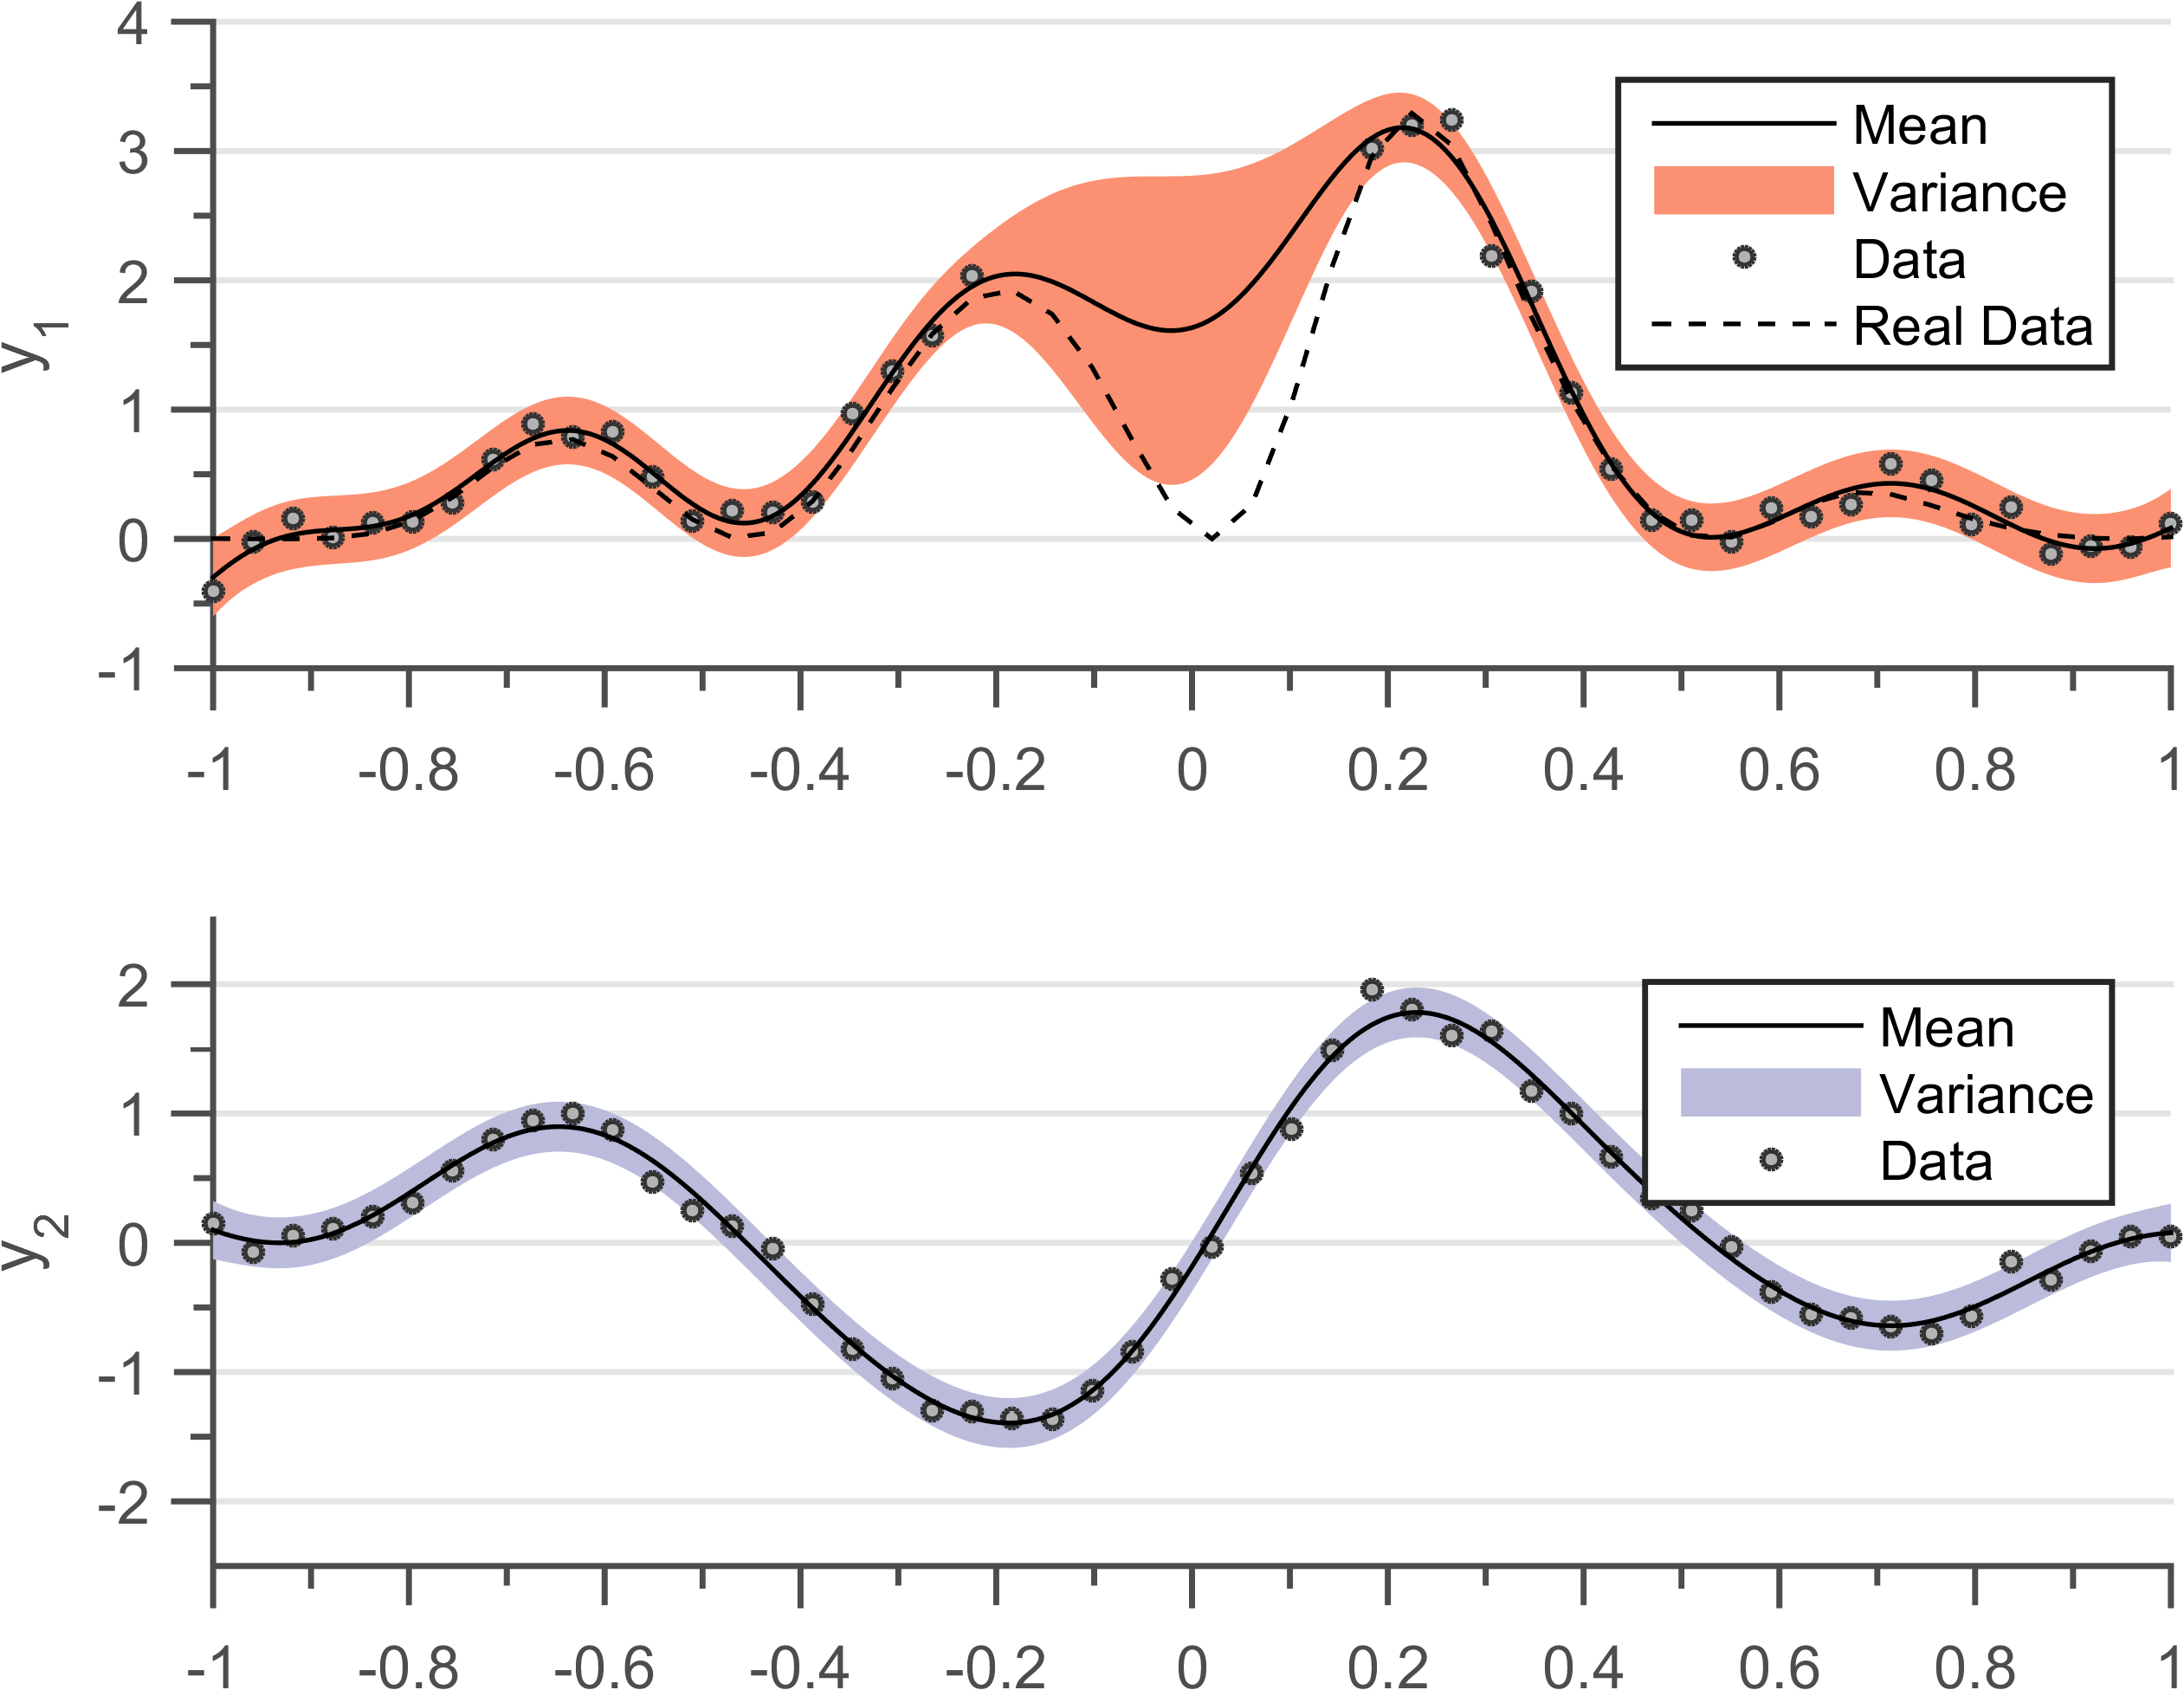
\includegraphics[width=0.3\textwidth]
  {images/part3/quadraticRelationshipMultiFidelityKernel}
  \label{subfigquadraticRelationshipMultiFidelityKernel}}
  \quad
  \subfigure[{Joint-GP Regression for the two outputs \(y^{1}\) and \(y^{2}\) related through equation \ref{eq:quadraticRelationship}. We can observe the improved prediction between zone with no data because information is being shared between the two outputs.}]
  {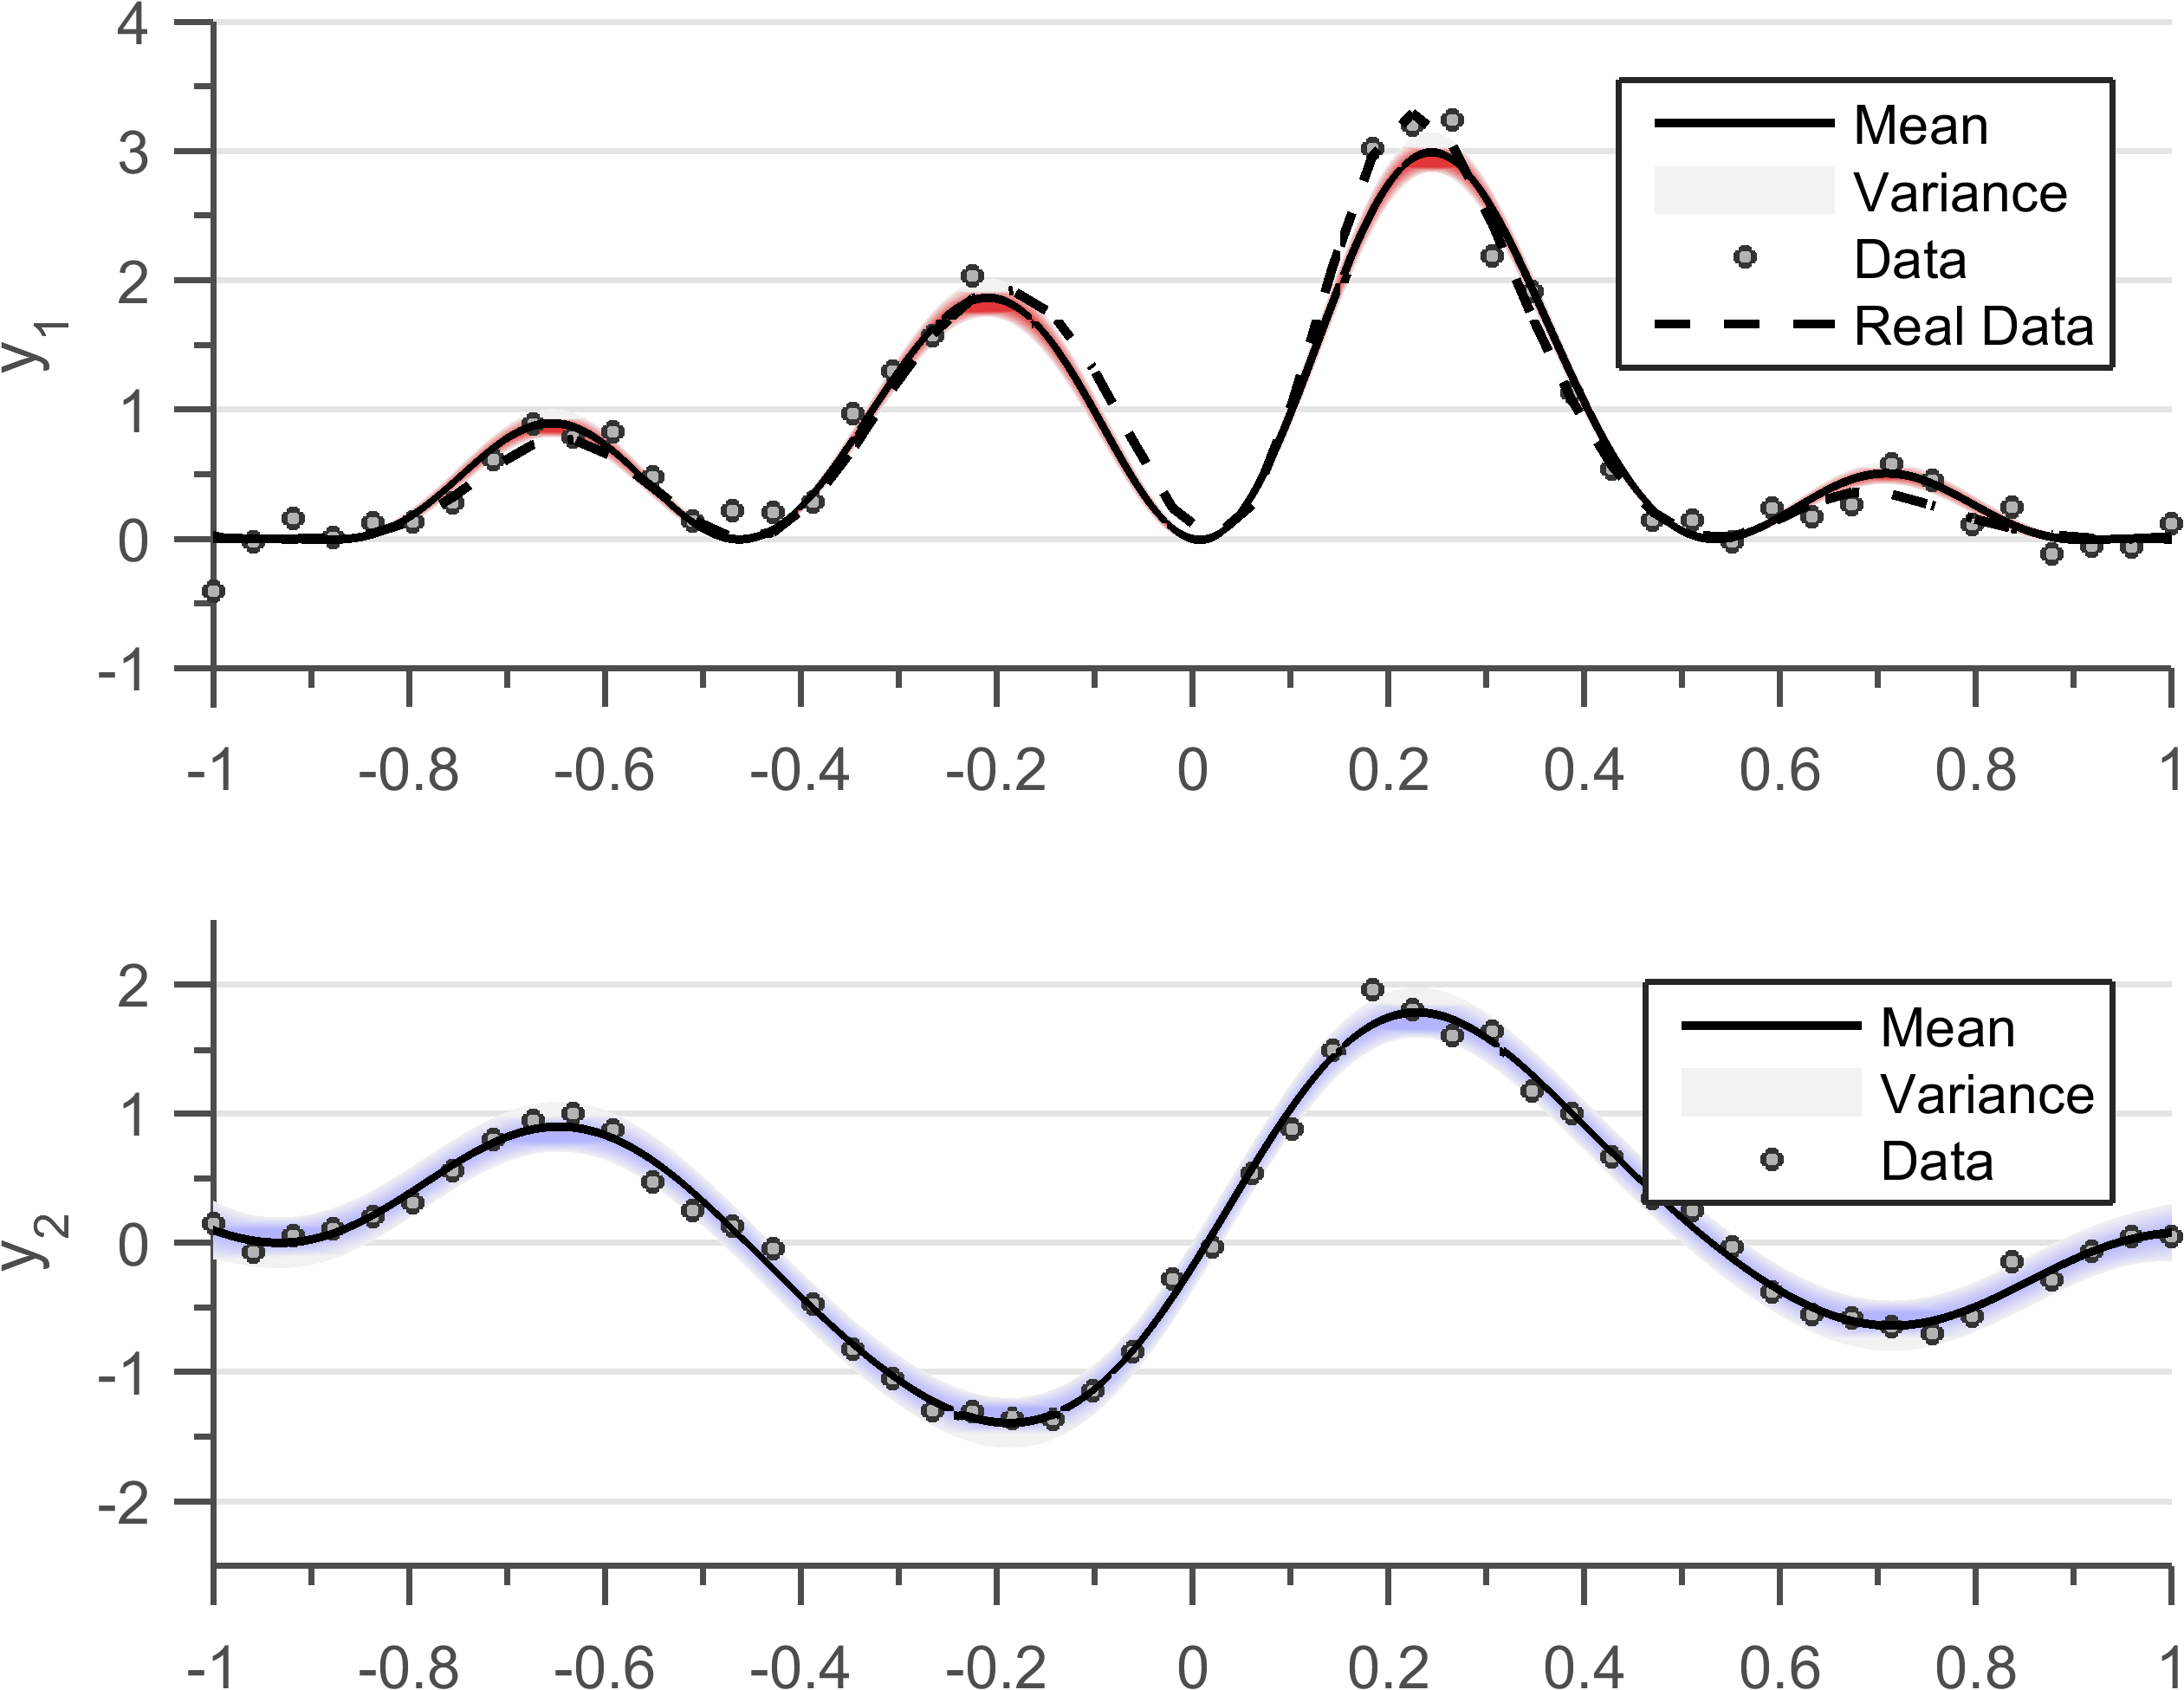
\includegraphics[width=0.3\textwidth]
  {images/part3/quadraticRelationshipJointKernel}
  \label{subfigquadraticRelationshipJointKernel}}
  
  \caption{GP Regression on Quadratic relationship. The solid black line represents the predicted mean while the shaded area denotes 2\(\sigma\) uncertainty region. The dashed black line represents the real value of \(f^{1}\) or \(f^{2}\). For \(y^{1}\) the data is hidden from section \(x = [-0.2, 0.2]\).}
  \label{figGPMOQuadraticRelationship}
\end{figure}

Table \ref{table:rmseY1Y2} shows comparison of Root Mean Square Error (RMSE). 10 sets of experiments were run for 85\% of data as training set and 15\% of data as the test set, test sets were removed uniformly from the output $y^1$ (similar to figure \ref{figGPMOQuadraticRelationship}). We learn the optimal set of hyperparameters for on training data all 10 sets of experiments. Finally, RMSE values are evaluated with respect to the test set. We are comparing here the accuracy of three model types, where the independent model gives the worst prediction, the multi-fidelity model is a little bit better but still worse than the model with the actual relationship enforced. 

\begin{table}
\caption{mean RMSE errors for quadratic relationship}
\centering
\label{t:observed_psrs}
\begin{tabular}{rcc}
\noalign{\smallskip} \hline \hline \noalign{\smallskip}
 & RMSE \(y^{1}\) & RMSE \(y^{2}\) \\
\hline
Independent Single-output GPR & 1.74 & 0.14 \\
Multi-fidelity GPR (section \ref{secMultiFidelityMTGP})& 1.54 & 0.13 \\
Joint Multi-output GPR & 0.26 & 0.12 \\
\noalign{\smallskip} \hline \noalign{\smallskip}
\end{tabular}
\label{table:rmseY1Y2}
\end{table}

The current experiment demonstrates how to enforce a non-linear relationship between outputs. Multi-fidelity GP has a similar performance as that of an independent GP since the two outputs are not results of code for different fidelities. Enforcing the quadratic relationship between the outputs has the best accuracy of the three methods (figure \ref{subfigquadraticRelationshipJointKernel}). 

\paragraph{Adding inequality constraints}
Research on adding inequality constraints in GP models is slowly picking up pace in the GP community. \cite{da2012gaussian} enforced inequality constraints by truncating probability distributions, while \cite{maatouk2017gaussian} enforce inequality constraints by using functional decomposition. The quadratic relationship gives rise to peculiar property. If  $f^{1} = \left [f^{2} \right]^2$ then it means that $f^{1} > 0$ $\forall x \in \mathcal{R}$, this property can also be used to indirectly enforce inequality constraints in GP models. 

Suppose we have access to a $N$ observed data-points $\mathcal{D} = \{\myMatrix{X}, \VEC{y}\}$ subject to the constraints $y_i > 0$ $\forall i \in N$. We can assume a second output $sqrtY$, such that $y = \left [sqrtY \right]^2$ and build a quadratic relationship enabled GP model between the two ($y$ and $sqrtY$). GP models enforcing monotonocity or convexity can be similarly made by first, enforcing a derivative relationship and then a quadratic relationship. 

One problem that can come up by enforcing inequality constraints using quadratic relationship, is that square root of $y$ ($sqrtY$) can be both positive and negative. This can complicate matters when calculating the mean of the square root. What are the implications of choosing one sign of square roots over the another needs more investigation. 

\subsection{Flight Mechanics on Flight Test Data}\label{sub:experimentsFlightLoadsData}
In this section, we conduct experiments applying our approach on the flight loads data. We look at normalized data of a simple longitudinal maneuver. The maneuver is quasi-static which means that airplane is in equilibrium at all times and there are no dynamic effects observed by the aircraft. The two outputs in our case are the coefficient of lift \(C_{z}\) on the Horizontal Tail Plane (HTP) and the spanwise lift \(k_{z}\). We know that the integral of spanwise pressure will be equal to the coefficient of lift (equation \ref{eq:relationCzKz}).

\begin{equation}\label{eq:relationCzKz}
\centering
C_{z}(\eta) = \int_{\eta_{edge}}^{\eta_{root}} k_{Z}(\eta)d\eta
\end{equation}.

Here, \(\eta_{edge}\) denotes the edge of horizontal tail span while \(\eta_{root}\) represents root of tail. The above equation is linear in nature and hence we will use equation \ref{eq:exactJointCovariance} to calculate the auto- and cross-covariance functions.

In practice, the coefficient of lift \(C_{z}\) is calculated using strain gauges on the HTP and the spanwise force is measured using pressure tappings. Chordwise pressures are measured at multiple \(\eta\) locations on the HTP, which are integrated chordwise to give spanwise lift distribution. We are trying to merge data coming from two different calculation chains flight mechanics (\(C_{z}\)) and aerodynamics (\(k_{z}\)), by using a basic physics based relationship between them. To the best of our knowledge this approach has not been proposed earlier in loads estimation.

Figure \ref{fig:cztzRelationship} shows a comparison between two joint multi-output GP on \(K_{z}\) and \(C_{z}\) using different prior distributions. Figure \ref{subfigKLPreFlightAndCzPreFlight_200_SE} shows the effect of SE kernel (infinite differentiability) on the joint model. The SE kernel is a strong assumption for the type of lift distribution. To accommodate for the value of measured \(C_{z}\), the error band increases and the boundary condition at HTP root is not satisfied. Moreover, we identify points in the figure \ref{subfigKLPreFlightAndCzPreFlight_200_SE} which fall out of the 95\% confidence band. We can claim with 95\% probability that if our lift distributions come from a family of infinitely differentiable functions these outliers do not satisfy the physics of the problem and can be termed as measurement errors.

Figure \ref{subfigKLPreFlightAndCzPreFlight_200_MAT5} shows the effect of twice differentiable Mat\'ern kernel on the joint model. The twice differentiable assumption gives our family of functions enough flexibility to follow the spanwise lift data. We observe that error estimates for \(C_{z}\) improve considerably while there is an increased uncertainty at the HTP root for \(K_{z}\). This loss in the order of differentiability can be explained due to fuselage HTP interaction near HTP root. We can conclude that even though we are working with very basic assumptions of differentiability the choice of kernel is important in performing the predictions. 

\begin{figure}[!ht]
  \centering
  \subfigure[{Joint multi-output GPR between \(K_{z}\) and \(C_{z}\) using a \textbf{SE kernel} and equation \ref{eq:relationCzKz}. Outlier points either do not follow the relationship between outputs or the SE kernel imposes a strict bias}]
  {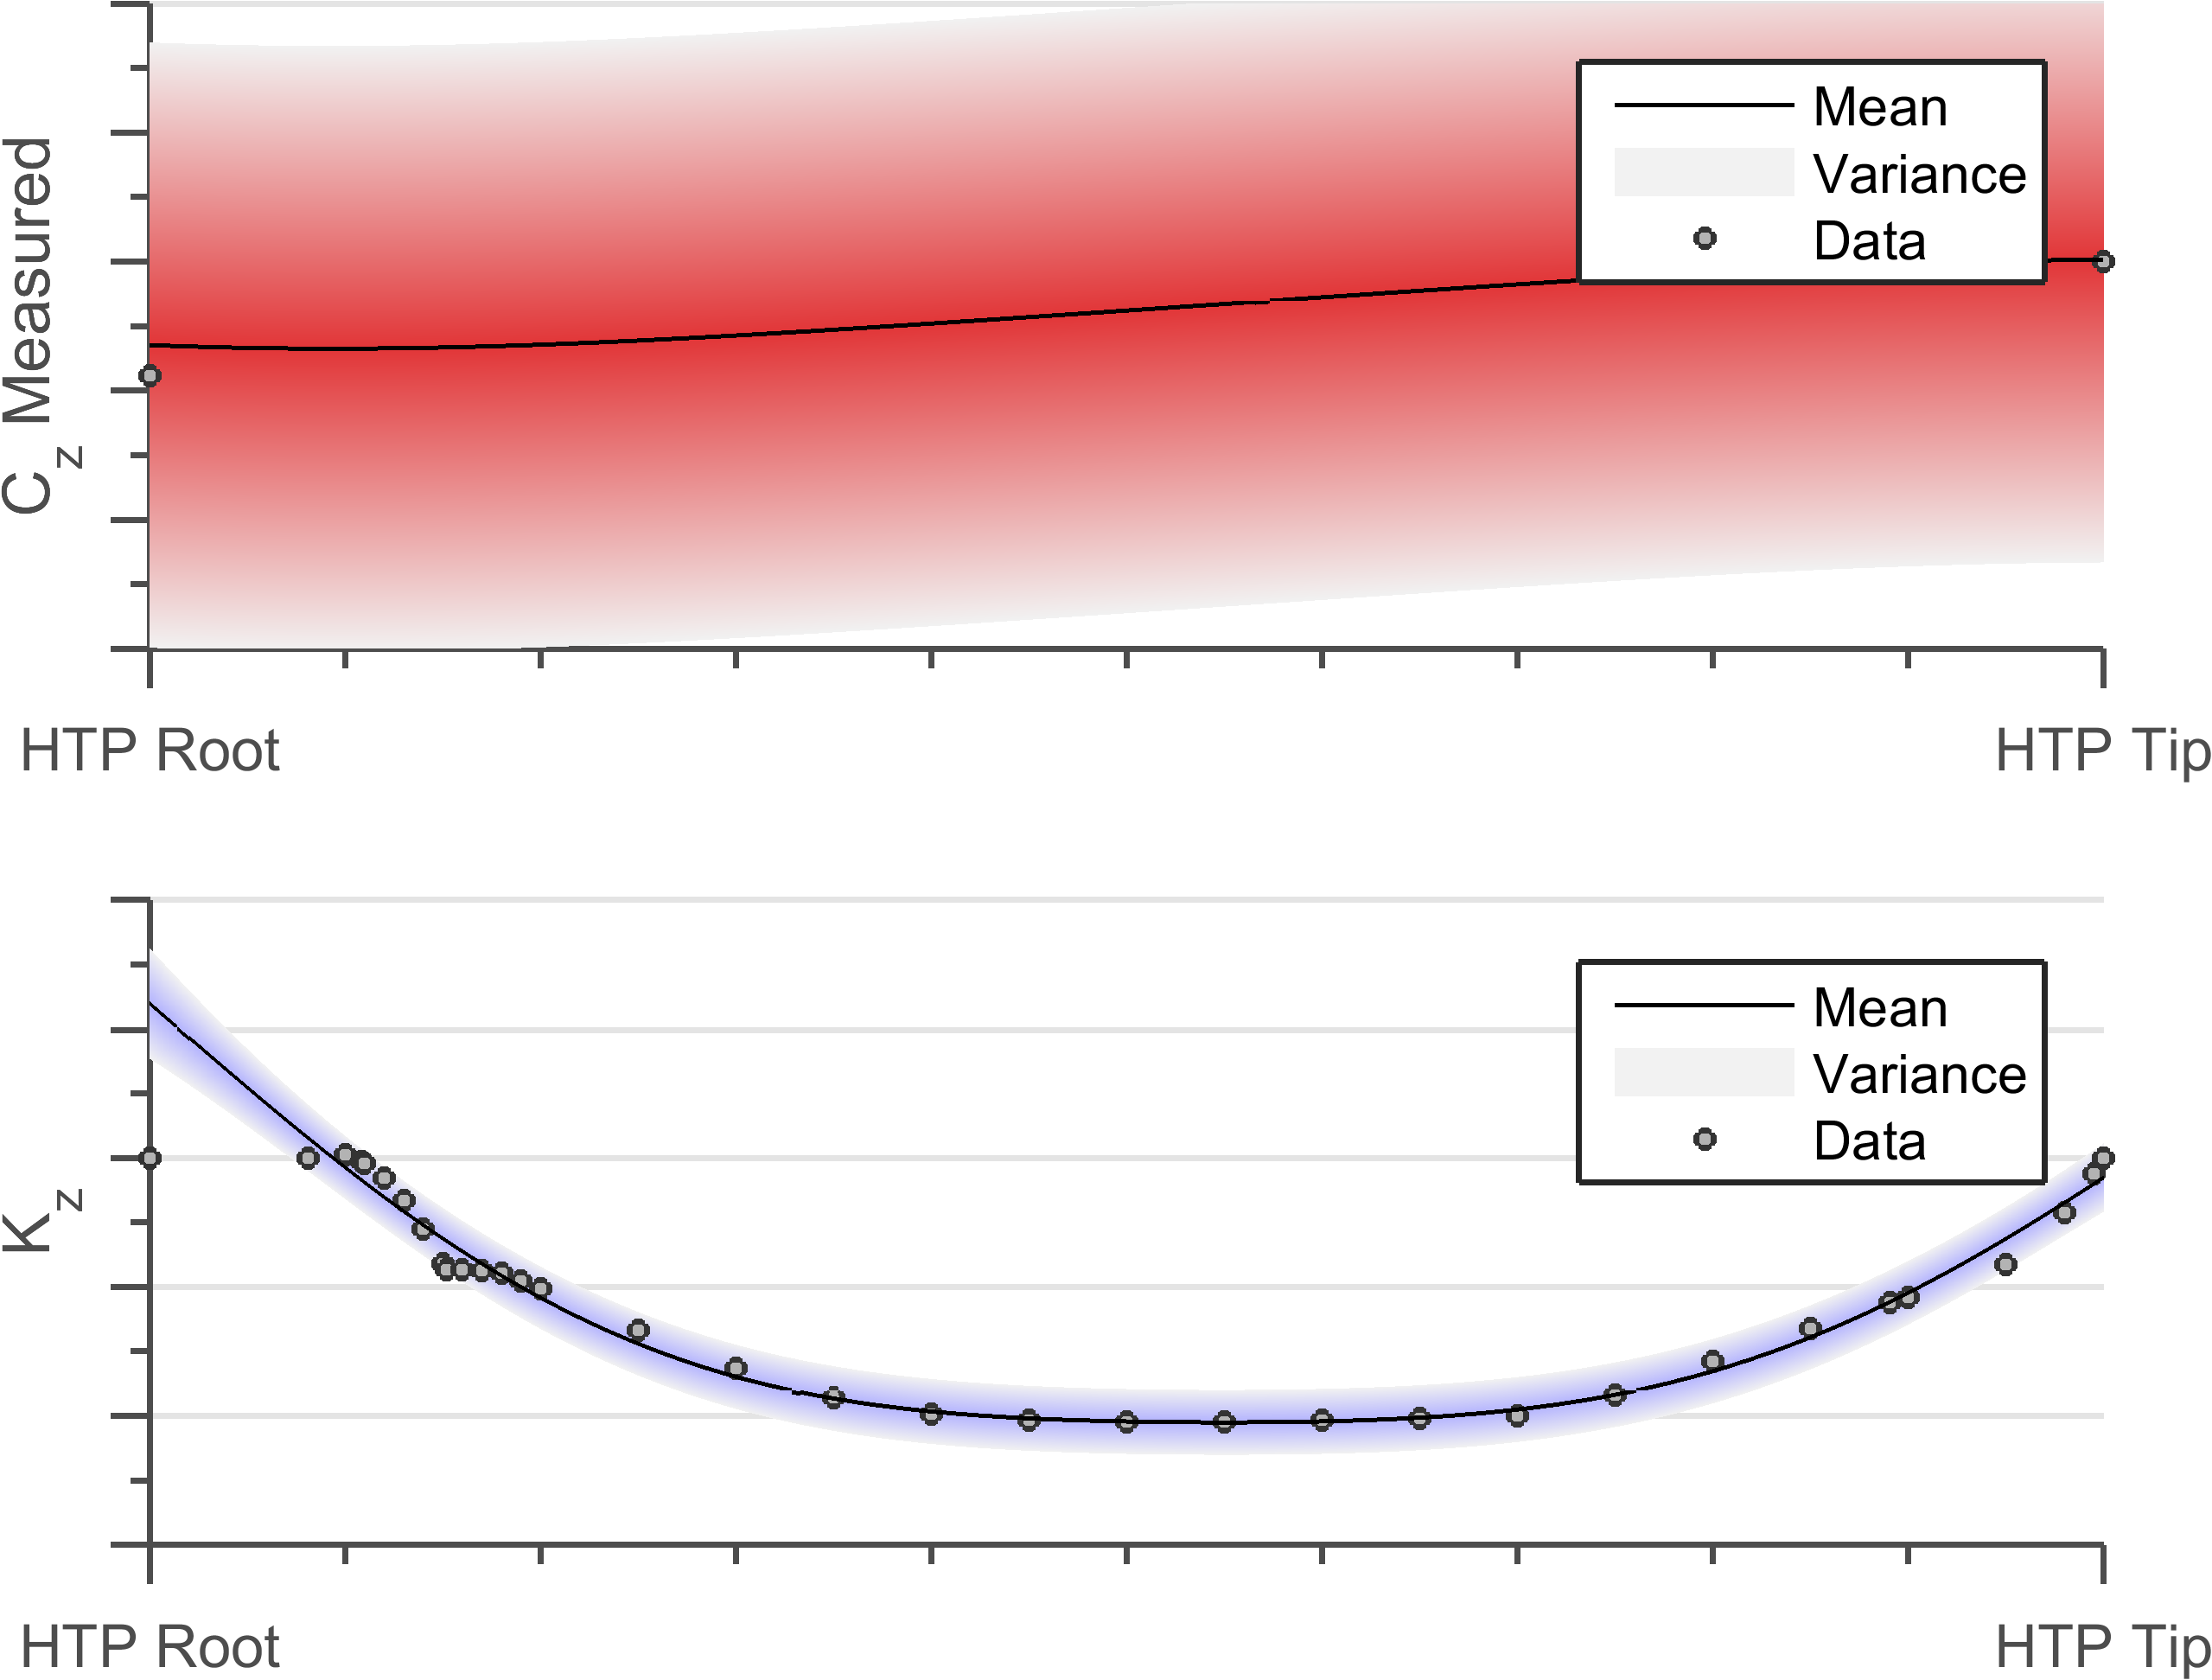
\includegraphics[width=0.45\textwidth]
  {images/part3/KLPreFlightAndCzPreFlight_200_SE}
  \label{subfigKLPreFlightAndCzPreFlight_200_SE}}
  \quad
  \subfigure[{Joint multi-output GPR between \(K_{z}\) and \(C_{z}\) using a twice differentiable \textbf{Mat\'ern kernel} and equation \ref{eq:relationCzKz}.}]
  {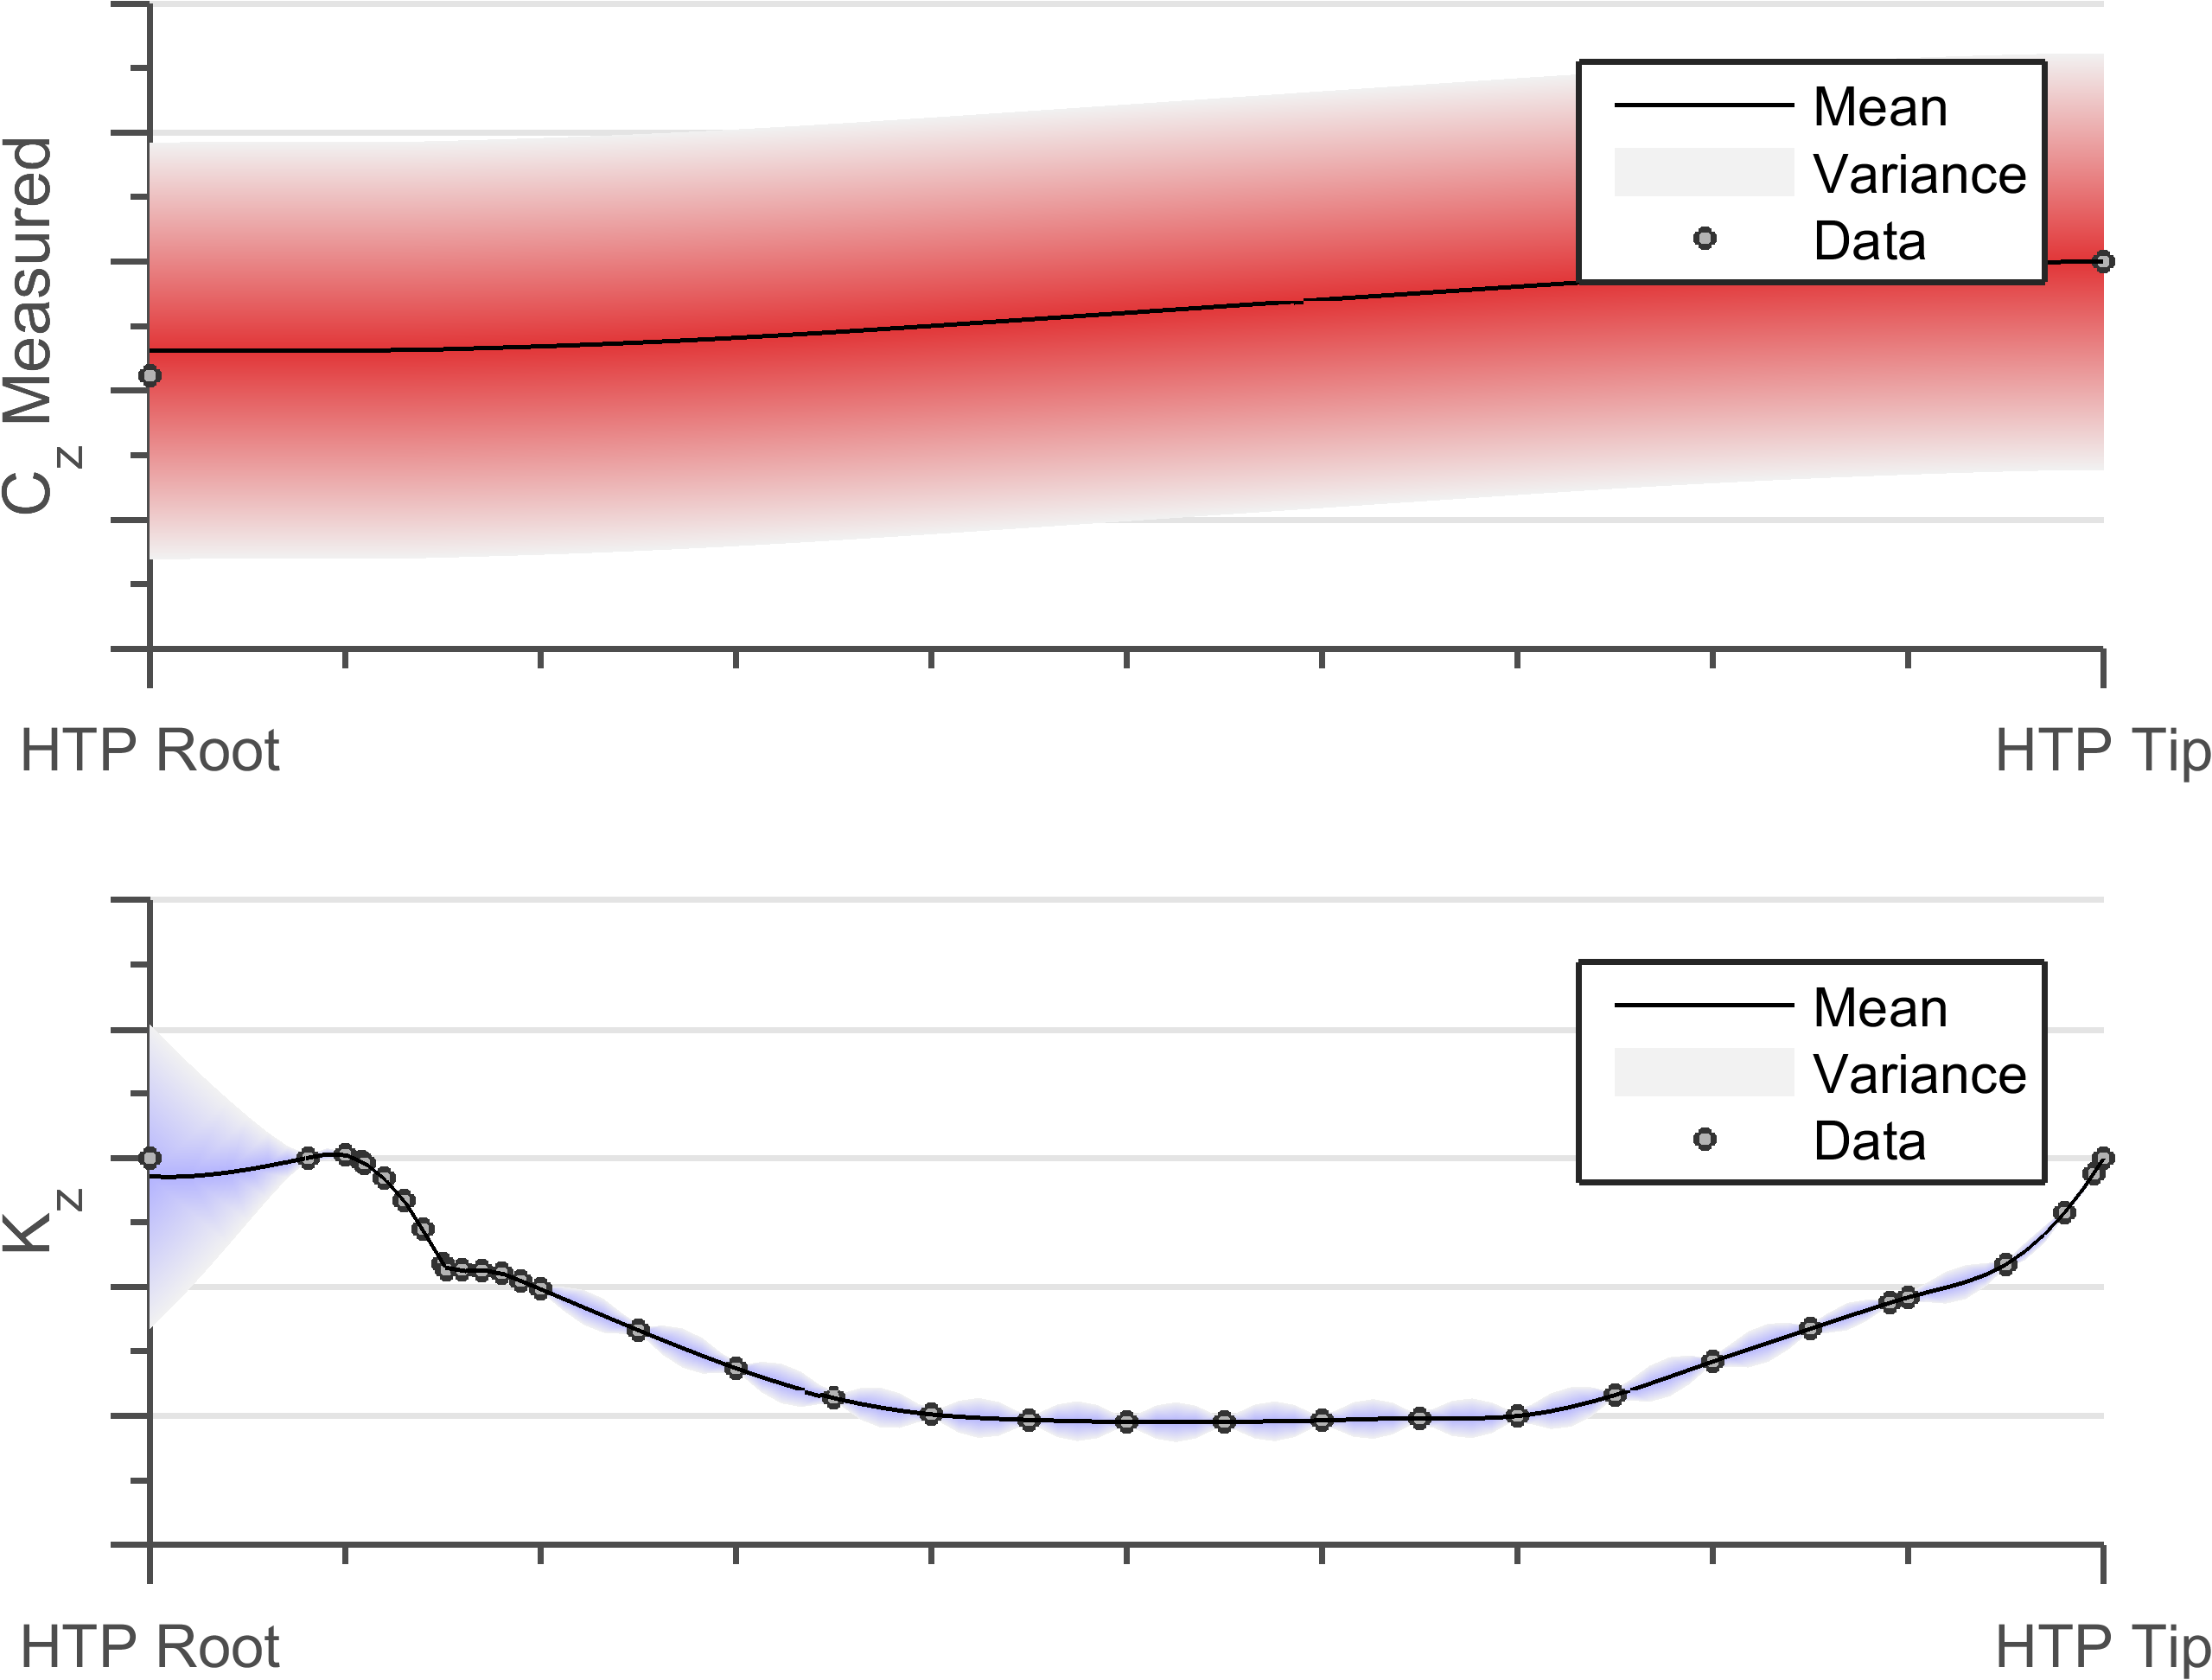
\includegraphics[width=0.45\textwidth]
  {images/part3/KLPreFlightAndCzPreFlight_200_MAT5}
  \label{subfigKLPreFlightAndCzPreFlight_200_MAT5}}
  \quad
\caption{Joint multi-output GPR on  \(K_{z}\) and \(C_{z}\) relationship. The solid black line represents the predicted mean while the shaded area denotes 2\(\sigma\) uncertainty region. The figure demonstrates the impact of the covariance function for relationship enabled regression.}
  \label{fig:cztzRelationship}
\end{figure}

In this section, we compare the predictive capabilities of using two different covariance functions for defining the prior of independent output $f^2$. For the current case, the SE kernel imposed a very strict bias for the pressure distribution $K_z$, this puts a few observation points outsize the 95\% confidence interval. In fact, the twice differentiable Mat\'ern kernel is a better covariance function for the problem. This is because due to the fuselage wing interaction, the pressure distribution is not infinitely differentiable near the HTP root. 

\paragraph{Identifying faulty sensors}
We also observe that the current formulation pushes observations that do not follow the physics of the system outside its confidence band, this is a very interesting property and can be used to automatically identify faulty sensors. Suppose we measure the loads on an aircraft using strain gauges, while we measure the acceleration of the aircraft using accelerometers. We can leverage the Newton's third law of motion ($\int loads = MassOfAircraft \times acceleration$) to build a robust loads model and identify faulty strain gauges automatically. 

Calculating the negative log-marginal likelihood involves inverting the matrix \(K_{XX} + \Sigma\). The size of the \(K_{XX} + \Sigma\) matrix depends on a total number of input points \(N\), hence inverting the matrix becomes intractable for a large number of input points. In the next section we describe how to solve the problem of inverting huge \(K_{XX} + \Sigma\) matrices using approximate inference techniques.

\section{Scaling up MTGP}\label{sec:sparseGPRegression}
As already discussed in chapter \ref{chapScalingGPR} on scaling GP regression, the GP approach is intractable for large datasets. For a multi-output GP as defined in section \ref{sub:MOGPs} the covariance matrix is of size \(N_{tot}\),  where \(\mathcal{O}\left ( N_{tot}^{3} \right )\) time is needed for inference and \(\mathcal{O}\left ( N_{tot}^{2} \right )\) memory for storage. 

This problem is further aggravated when we are creating a joint Gram matrix between several outputs. In this section, we extend the formulation of variational GP approximation (section \ref{subSecVariationalApprox}) and distributed GP approximation (section \ref{secDgp}) for the case of MTGP's. The results of this study were published in ICPRAM 2016 and LNCS 2017 \cite{icpram16Ankit, oatao18000}. The remaining section details the two methods for approximating covariance matrix which can be later used to calculate the predictive mean, predictive covariance and the marginal likelihood (\ref{eq:predictiveMOMeanCh7}, \ref{eq:predictiveMOCovarianceCh7} and \ref{eq:exactMONLML}).

\begin{comment}
Inverting the covariance matrix takes a considerable amount of time and memory during the process. Hence, almost all techniques to approximate inference try and approximate the inversion of covariance matrix \(K_{XX}\). If a covariance matrix is diagonal or block-diagonal in nature then methods such as the mixture of experts are used eg. distributed GP. Whereas if the covariance matrix is more spread out and has similar terms in its cross diagonals then low-rank approximations are used eg. variational approximation. 
\end{comment}

\subsection{Variational Approximation on Multi-output GP}\label{sec:varMOGP}
Sparse methods use a small set of \(m\) function points as support or inducing variables. Suppose we use \(m\) inducing variables to construct our sparse GP. The inducing variables are the latent function values evaluated at inputs \(x_{M}\). An approximation to the true log marginal likelihood in equation \ref{eq:exactMONLML} can allow us to infer these quantities.

We try to approximate the joint-posterior distribution \(p(X| Y)\) by introducing a variational distribution \(q(X)\). In the case of varying number of inputs for different outputs, we place the inducing points over the modified input space (equation \ref{eq:modifiedInput}) and extend the derivation of \cite{Titsias09variationallearning} to the multi-output case. 

\begin{equation}\label{eq:multiVariationalQ}
 q(X) = \mathcal{N}(X|  \mu, A)
\end{equation}
 
Here \(\mu\) and \(A\) are parameters of the variational distribution. We follow the derivation provided in \cite{Titsias09variationallearning} and obtain the lower bound ($Fv$) of true marginal likelihood.

\begin{equation}\label{eq:lowerBoundMultiVarNLML}
F_{V} = log(\mathcal{N}[Y| 0, \sigma ^{2}I + K_{Nystrom}]) - \frac{1}{2\sigma ^{2}}Tr(\tilde{K})
\end{equation}

where \(K_{Nystrom} = K_{XX_{M}}K_{X_{M}X_{M}}^{-1}K_{X_{M}X}\) and \(\tilde{K} = K_{XX} - K_{Nystrom}\). \(K_{XX}\) is the joint-covariance matrix derived using equation \ref{eq:exactJointCovariance} using the input vector \(X\). \(K_{X_{M}X_{M}}\) is the joint-covariance function on the inducing points \(X_{M}\), such that \(X_{M} = [x_{M1}, x_{M2}, ..., x_{M2}]\). While \(K_{XX_{M}}\) is the cross-covariance matrix between \(X_{joint}\) and \(X_{M}\). 

Figure \ref{subfig:nystormJointmatrixRandom3} shows the Gram matrix after performing the Nystr\"{o}m approximation for the Gram matrix described in the left figure. We see how choosing three same random inducing points for both the outputs ($y^1$ and $y^2$) impacts the Gram matrix. As analyzed in the chapter \ref{chapScalingGPR} we can improve the approximate Gram matrix if we increase the number of inducing points. 

\begin{figure}[!ht]
  \centering
  \subfigure[{Gram matrix between \(y^1\) and \(y^2\) such that \(y^1 = \int_{0}^{x} y^2\). SE covariance function is used for the $y^2$ with $\theta = [1, 0.2]$, and $\myMatrix{X^j} = [0:0.01, 1]$ $\forall$ $j=[1, 2]$ (figure\ref{subfig:integralGramMatrix})} ]
  {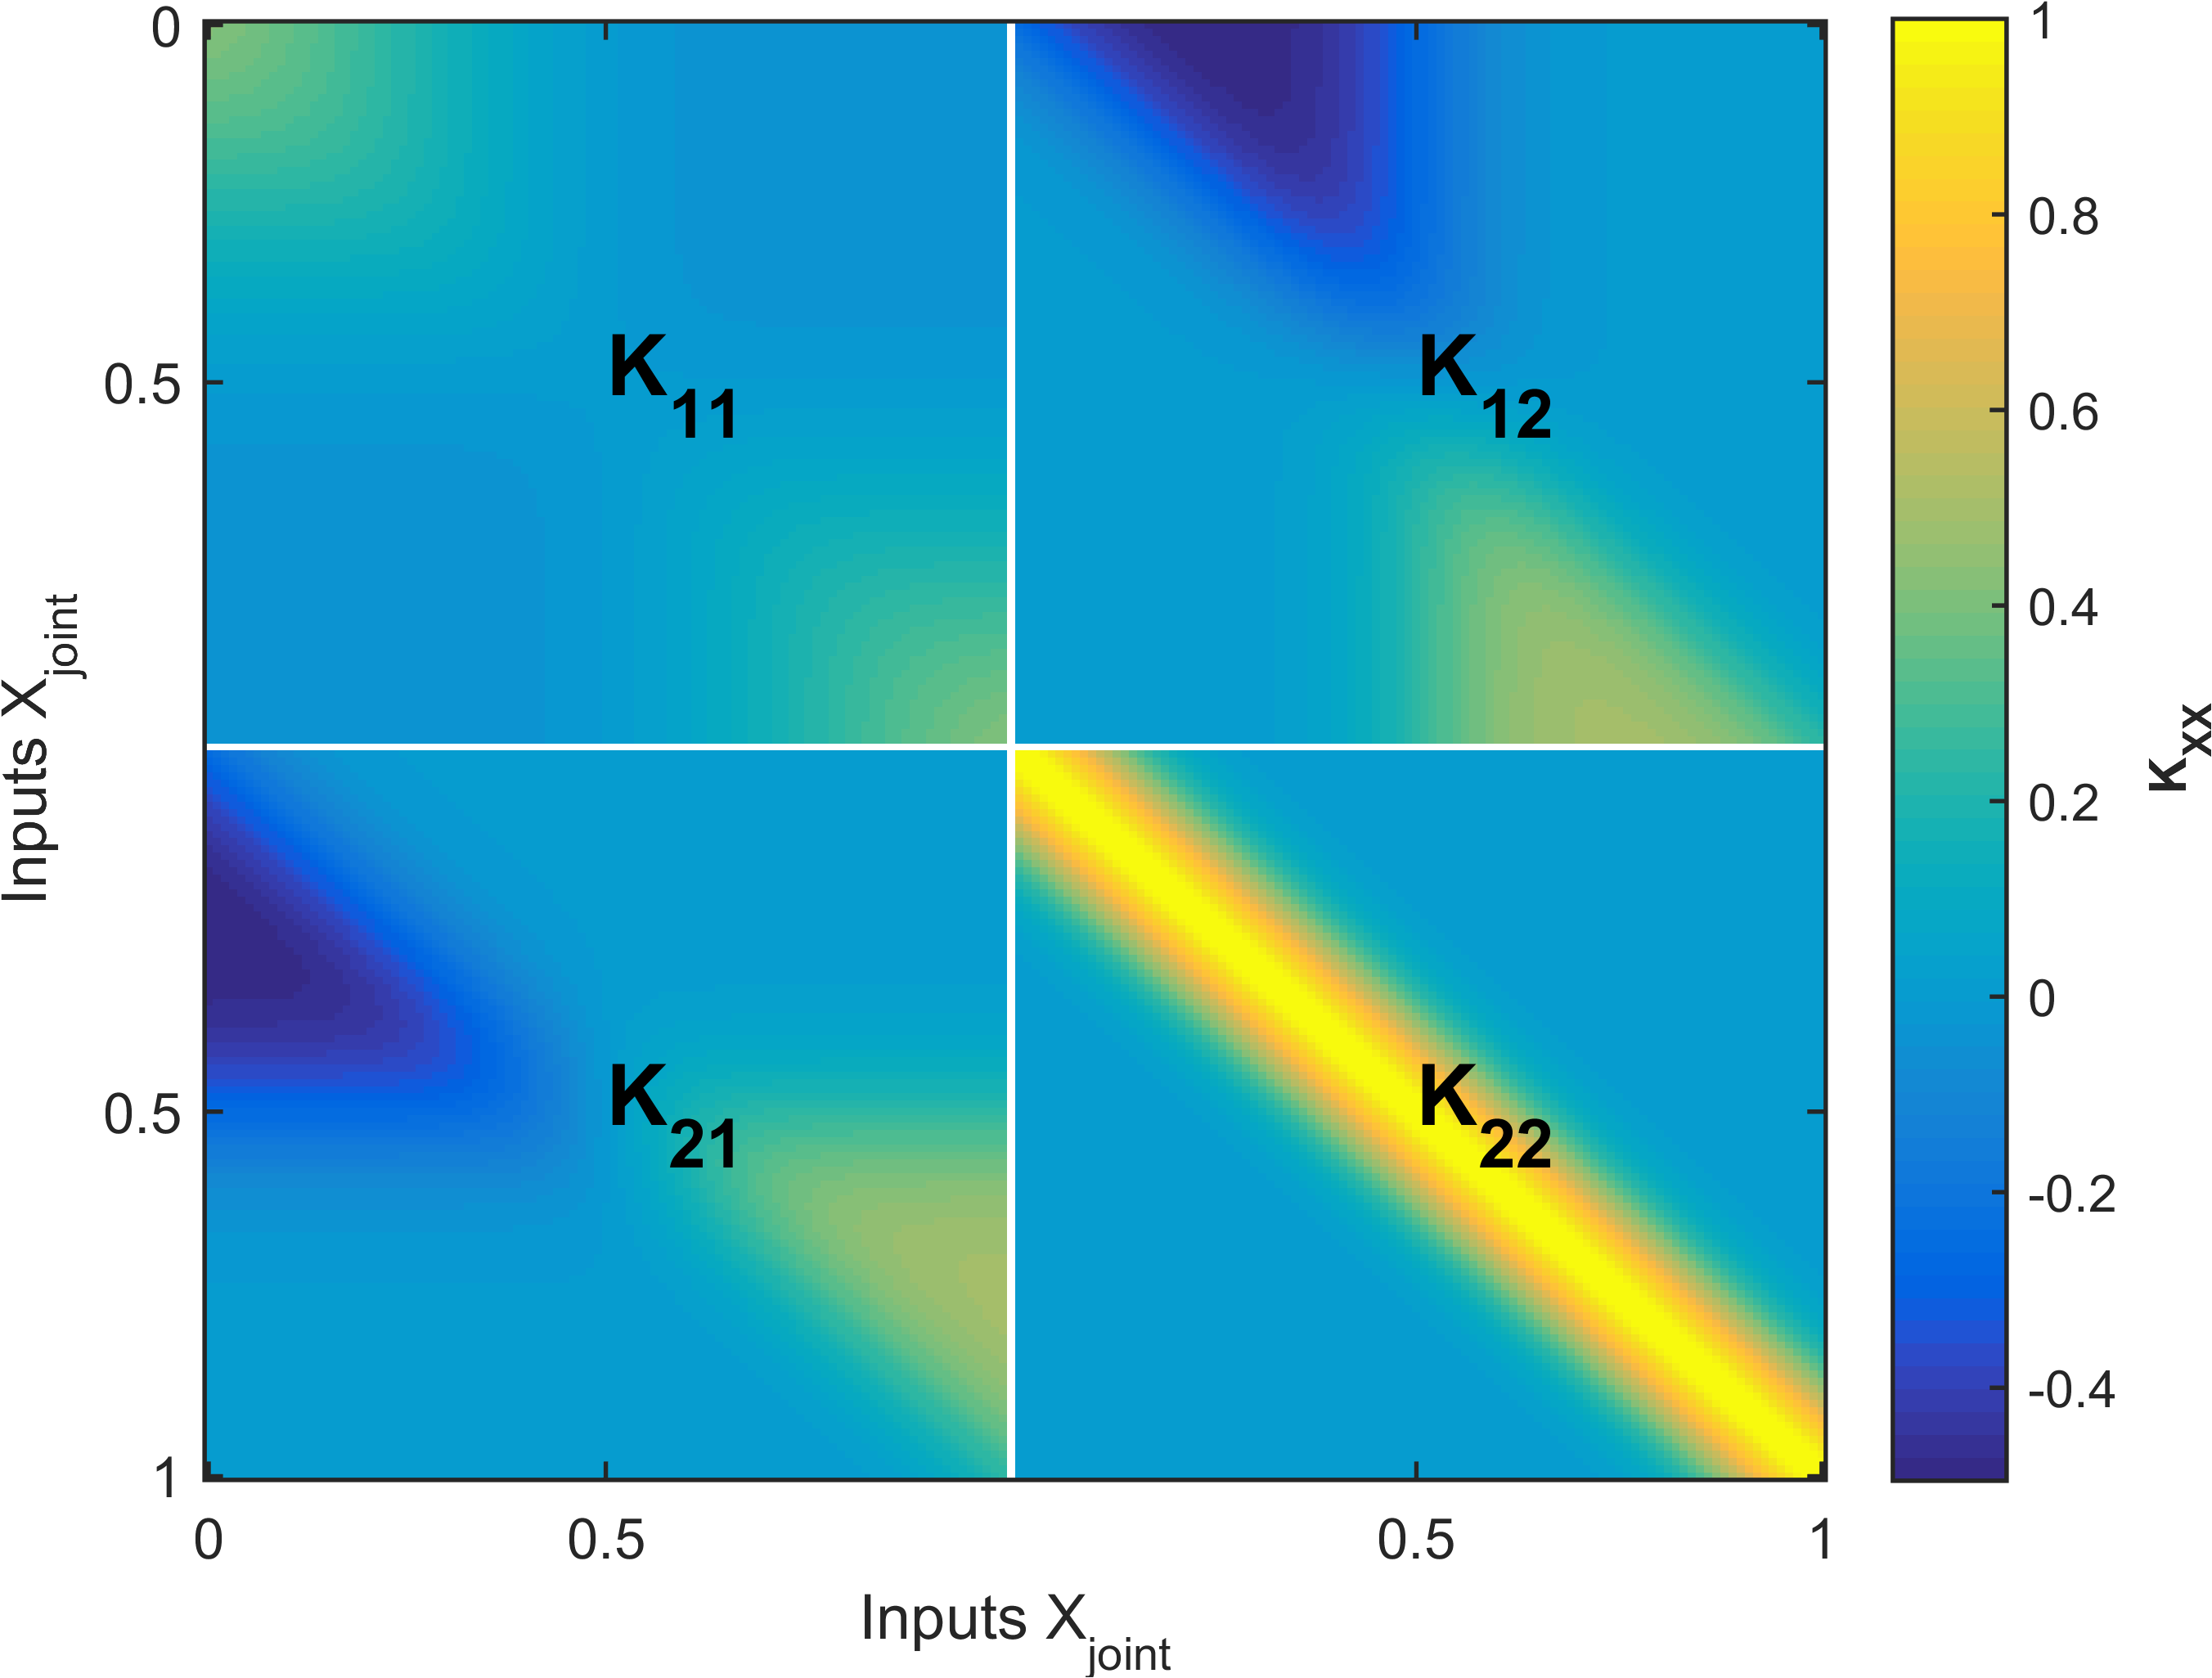
\includegraphics[width=0.45\textwidth]
  {images/part3/integralGramMatrix}}\quad
  \subfigure[{Approximated Gram matrix using Nystr\"{o}m approximation for Gram matrix of figure in left. Three inducing points were chosen randomly, the white lines denote the location of inducing points.}]
  {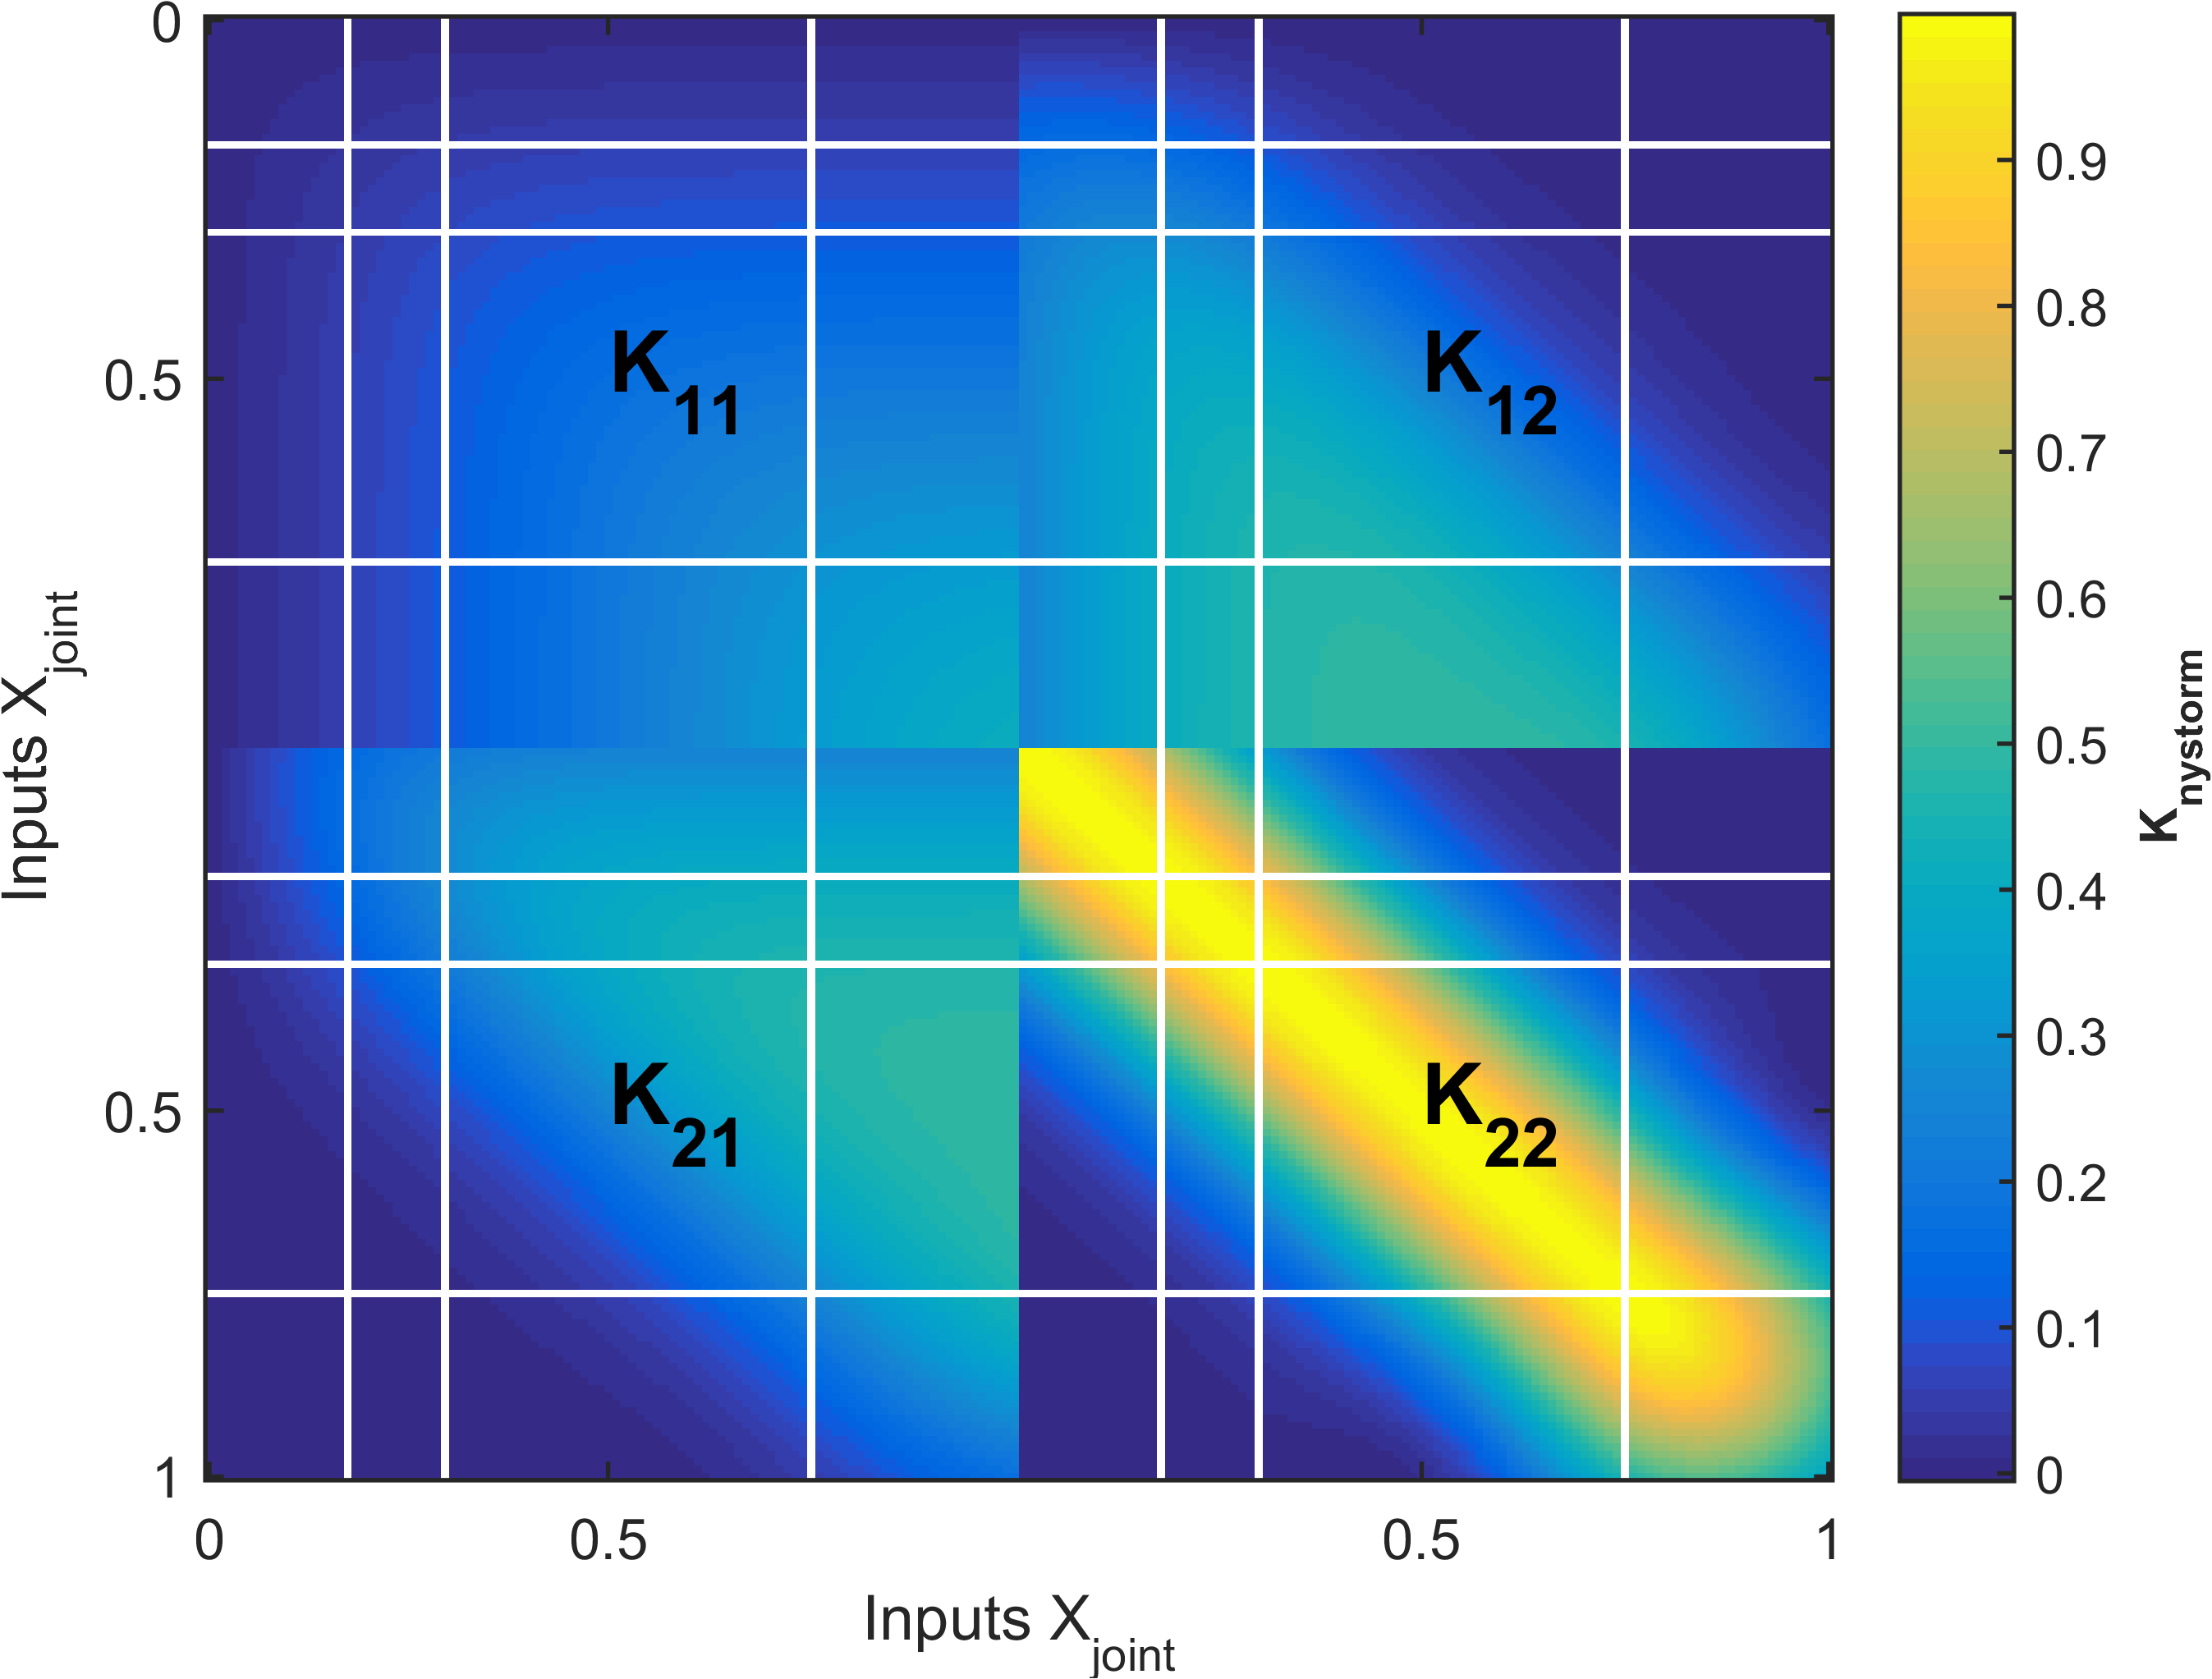
\includegraphics[width=0.45\textwidth]
  {images/part3/nystormJointmatrixRandom3}
  \label{subfig:nystormJointmatrixRandom3}}
  \caption{Approximate Gram matrix for a Joint MTGP kernel using Nystr\"{o}m approximation}
\end{figure}

The bound ($Fv$) can be maximized with respect to all parameters of the covariance function; the model hyperparameters and the variational parameters. The optimization parameters are the inducing inputs \(x_{M}\), the hyperparameters \(\theta\) of the independent covariance matrix \(K_{22}\) and the error while measuring the outputs \(\sigma\). There is a trade-off between quality of the estimate and amount of time taken for the estimation process. On the one hand the number of inducing points determine the value of optimized negative log-marginal likelihood and hence the quality of the estimate. While, on the other hand there is a computational load of \(\mathcal{O}\left ( N(MD_{outputs})^{2} \right )\) for inference. We increase the number of inducing points until the difference between two successive likelihoods is below a predefined quantity.   

\subsection{Distributed Inference on Multi-output GP}\label{sec:dMOGP}
An alternative to sparse approximations is to learn local experts on a subset of data. We have described distributed GP in detail in section \ref{secDgp}. We again distribute our dataset $X_{joint}$ into smaller experts and use the independence assumption between experts to approximate the Gram matrix.  Figure \ref{figDGPMTGP} shows the difference between an exact Gram matrix and a Gram matrix approximated using distributed GP.

Figure \ref{subfig:distributedJointmatrixUniform} shows the Gram matrix after performing distributed approximation for the Gram matrix described in the left figure. We see how choosing two same uniform experts for both the outputs ($y^1$ and $y^2$) impact the Gram matrix. As analyzed in the chapter \ref{chapScalingGPR}, we can improve the approximate Gram matrix if we increase the number of experts. 

\begin{figure}[!ht]
  \centering
  \subfigure[{Gram matrix between \(y^1\) and \(y^2\) such that \(y^1 = \int_{0}^{x} y^2\). SE covariance function is used for the $y^2$ with $\theta = [1, 0.2]$, and $\myMatrix{X^j} = [0:0.01, 1]$ $\forall$ $j=[1, 2]$ (figure\ref{subfig:integralGramMatrix})}]
  {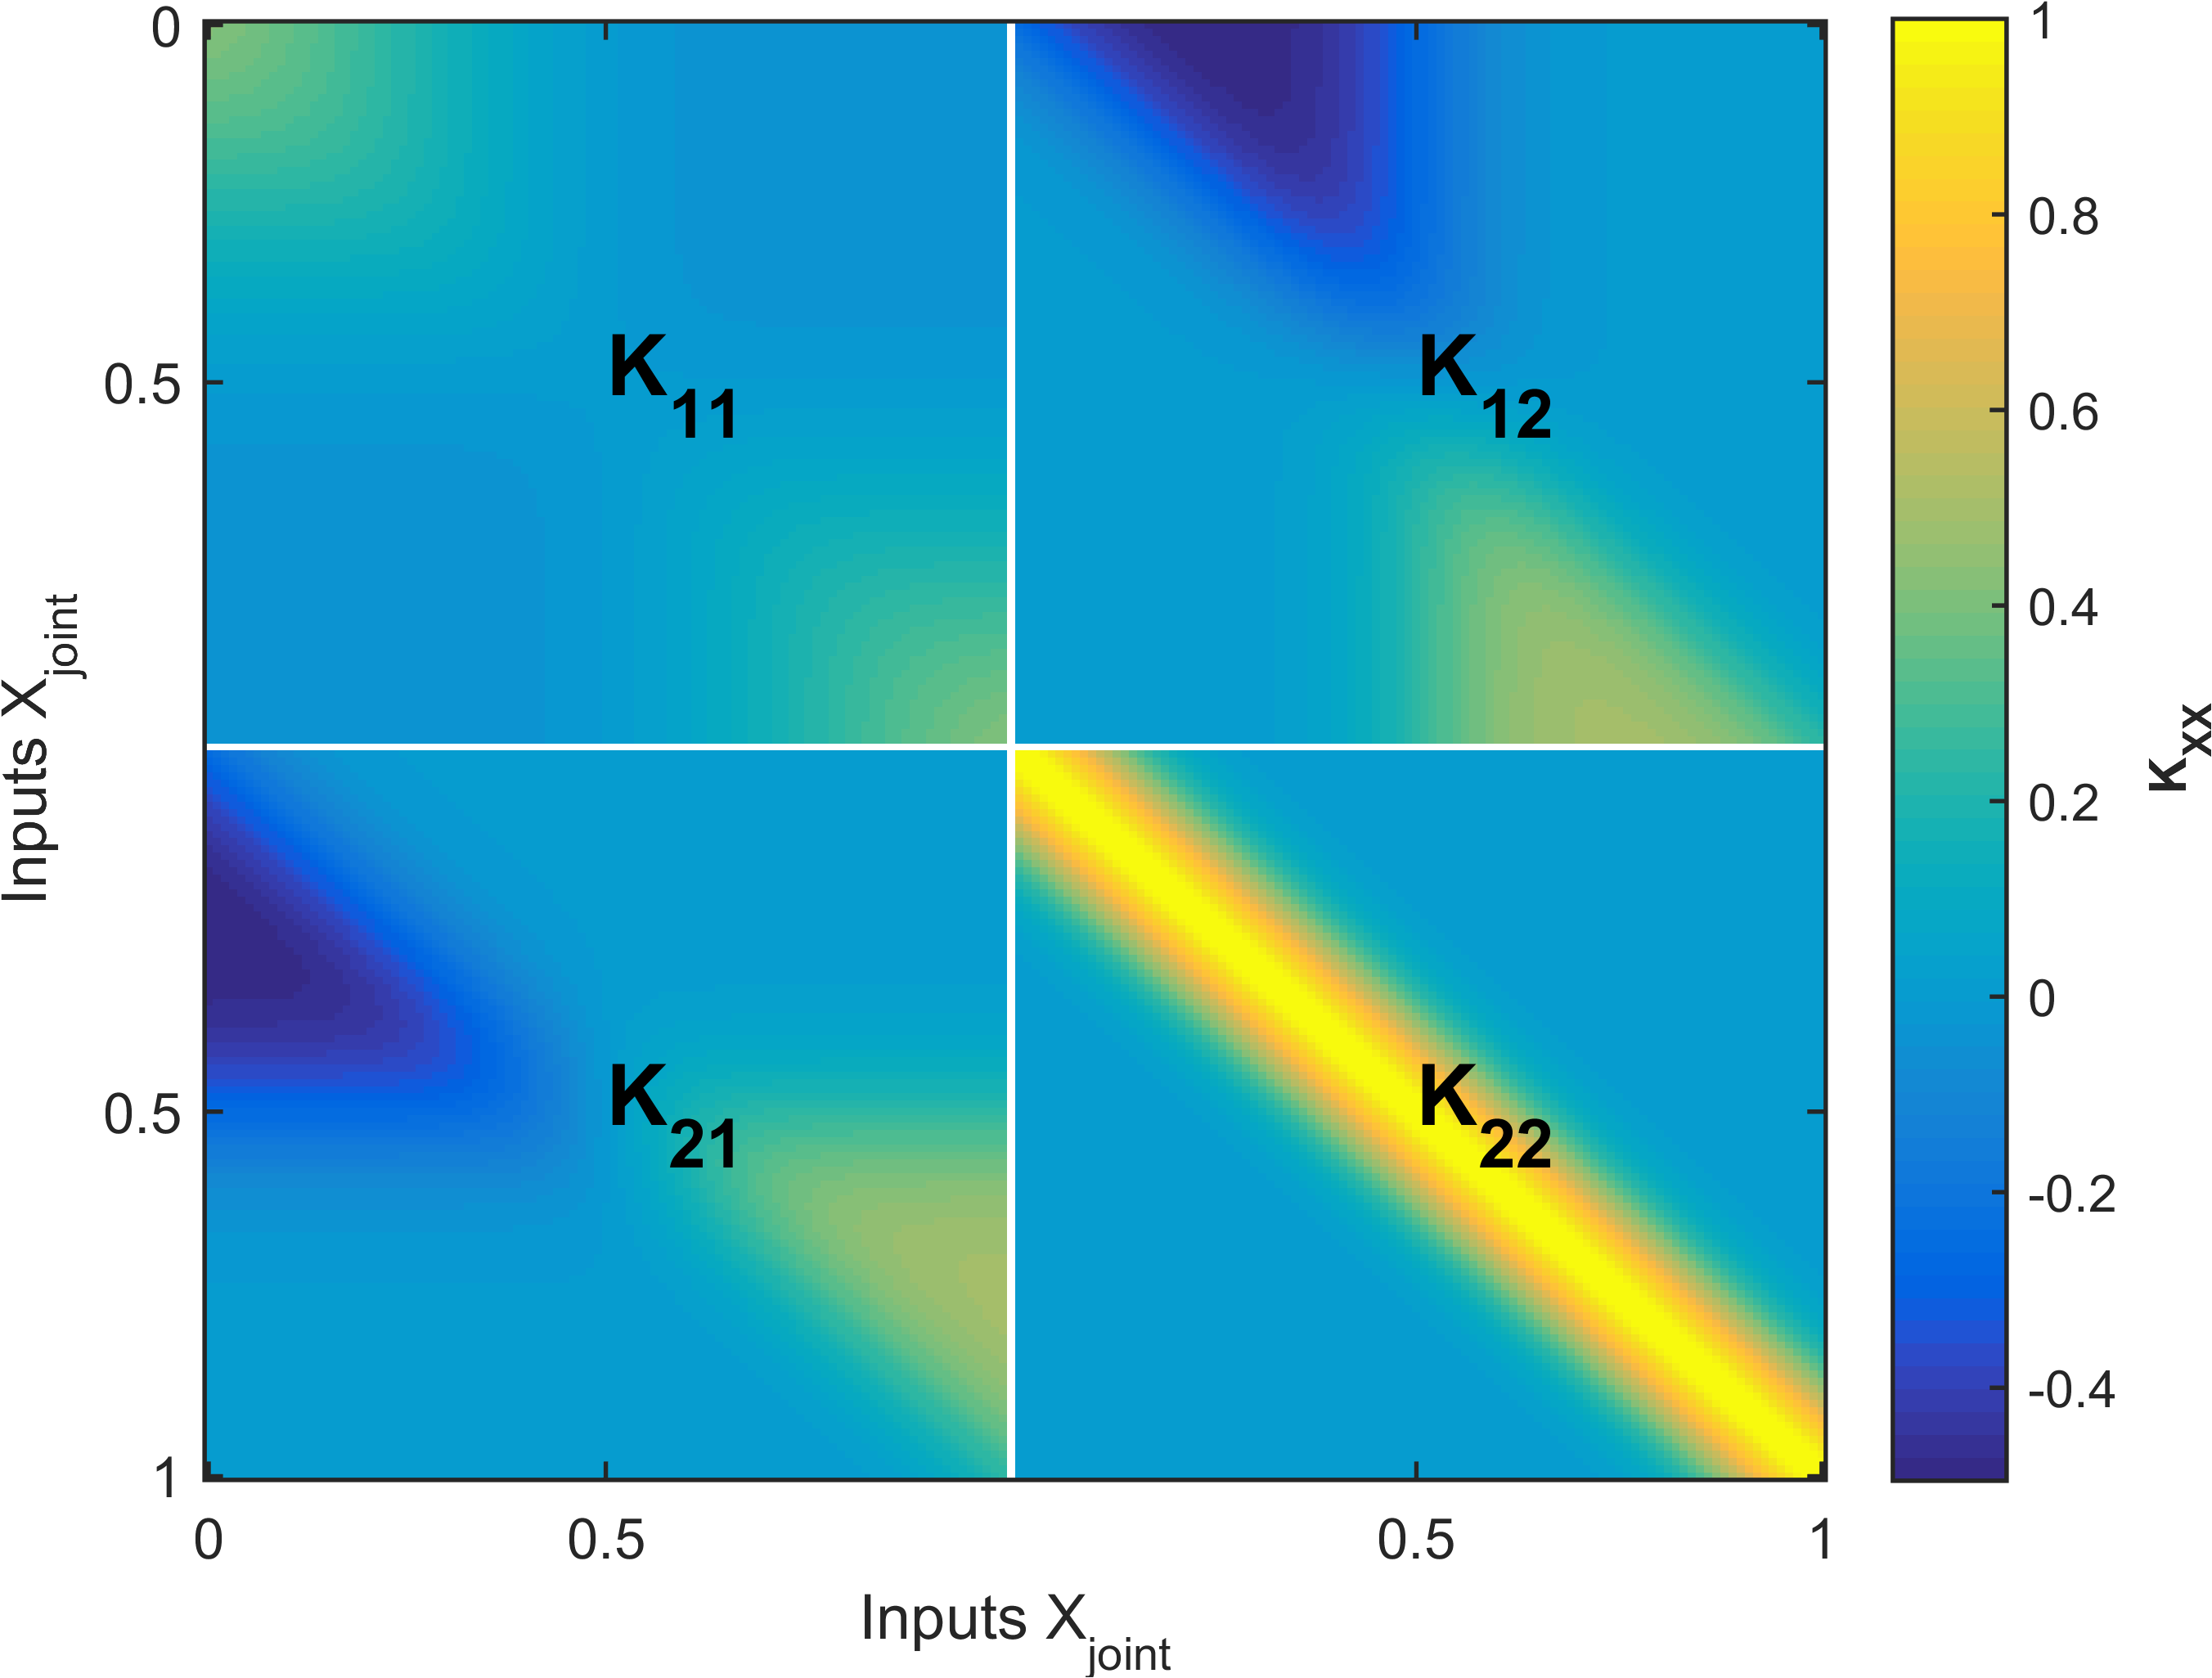
\includegraphics[width=0.45\textwidth]
  {images/part3/integralGramMatrix}}
  \quad
  \subfigure[Approximated Gram matrix using distributed GP approximation for Gram matrix of figure in left. Points in the experts are distributed uniformly. We can observe that covariance across experts goes to zero]
  {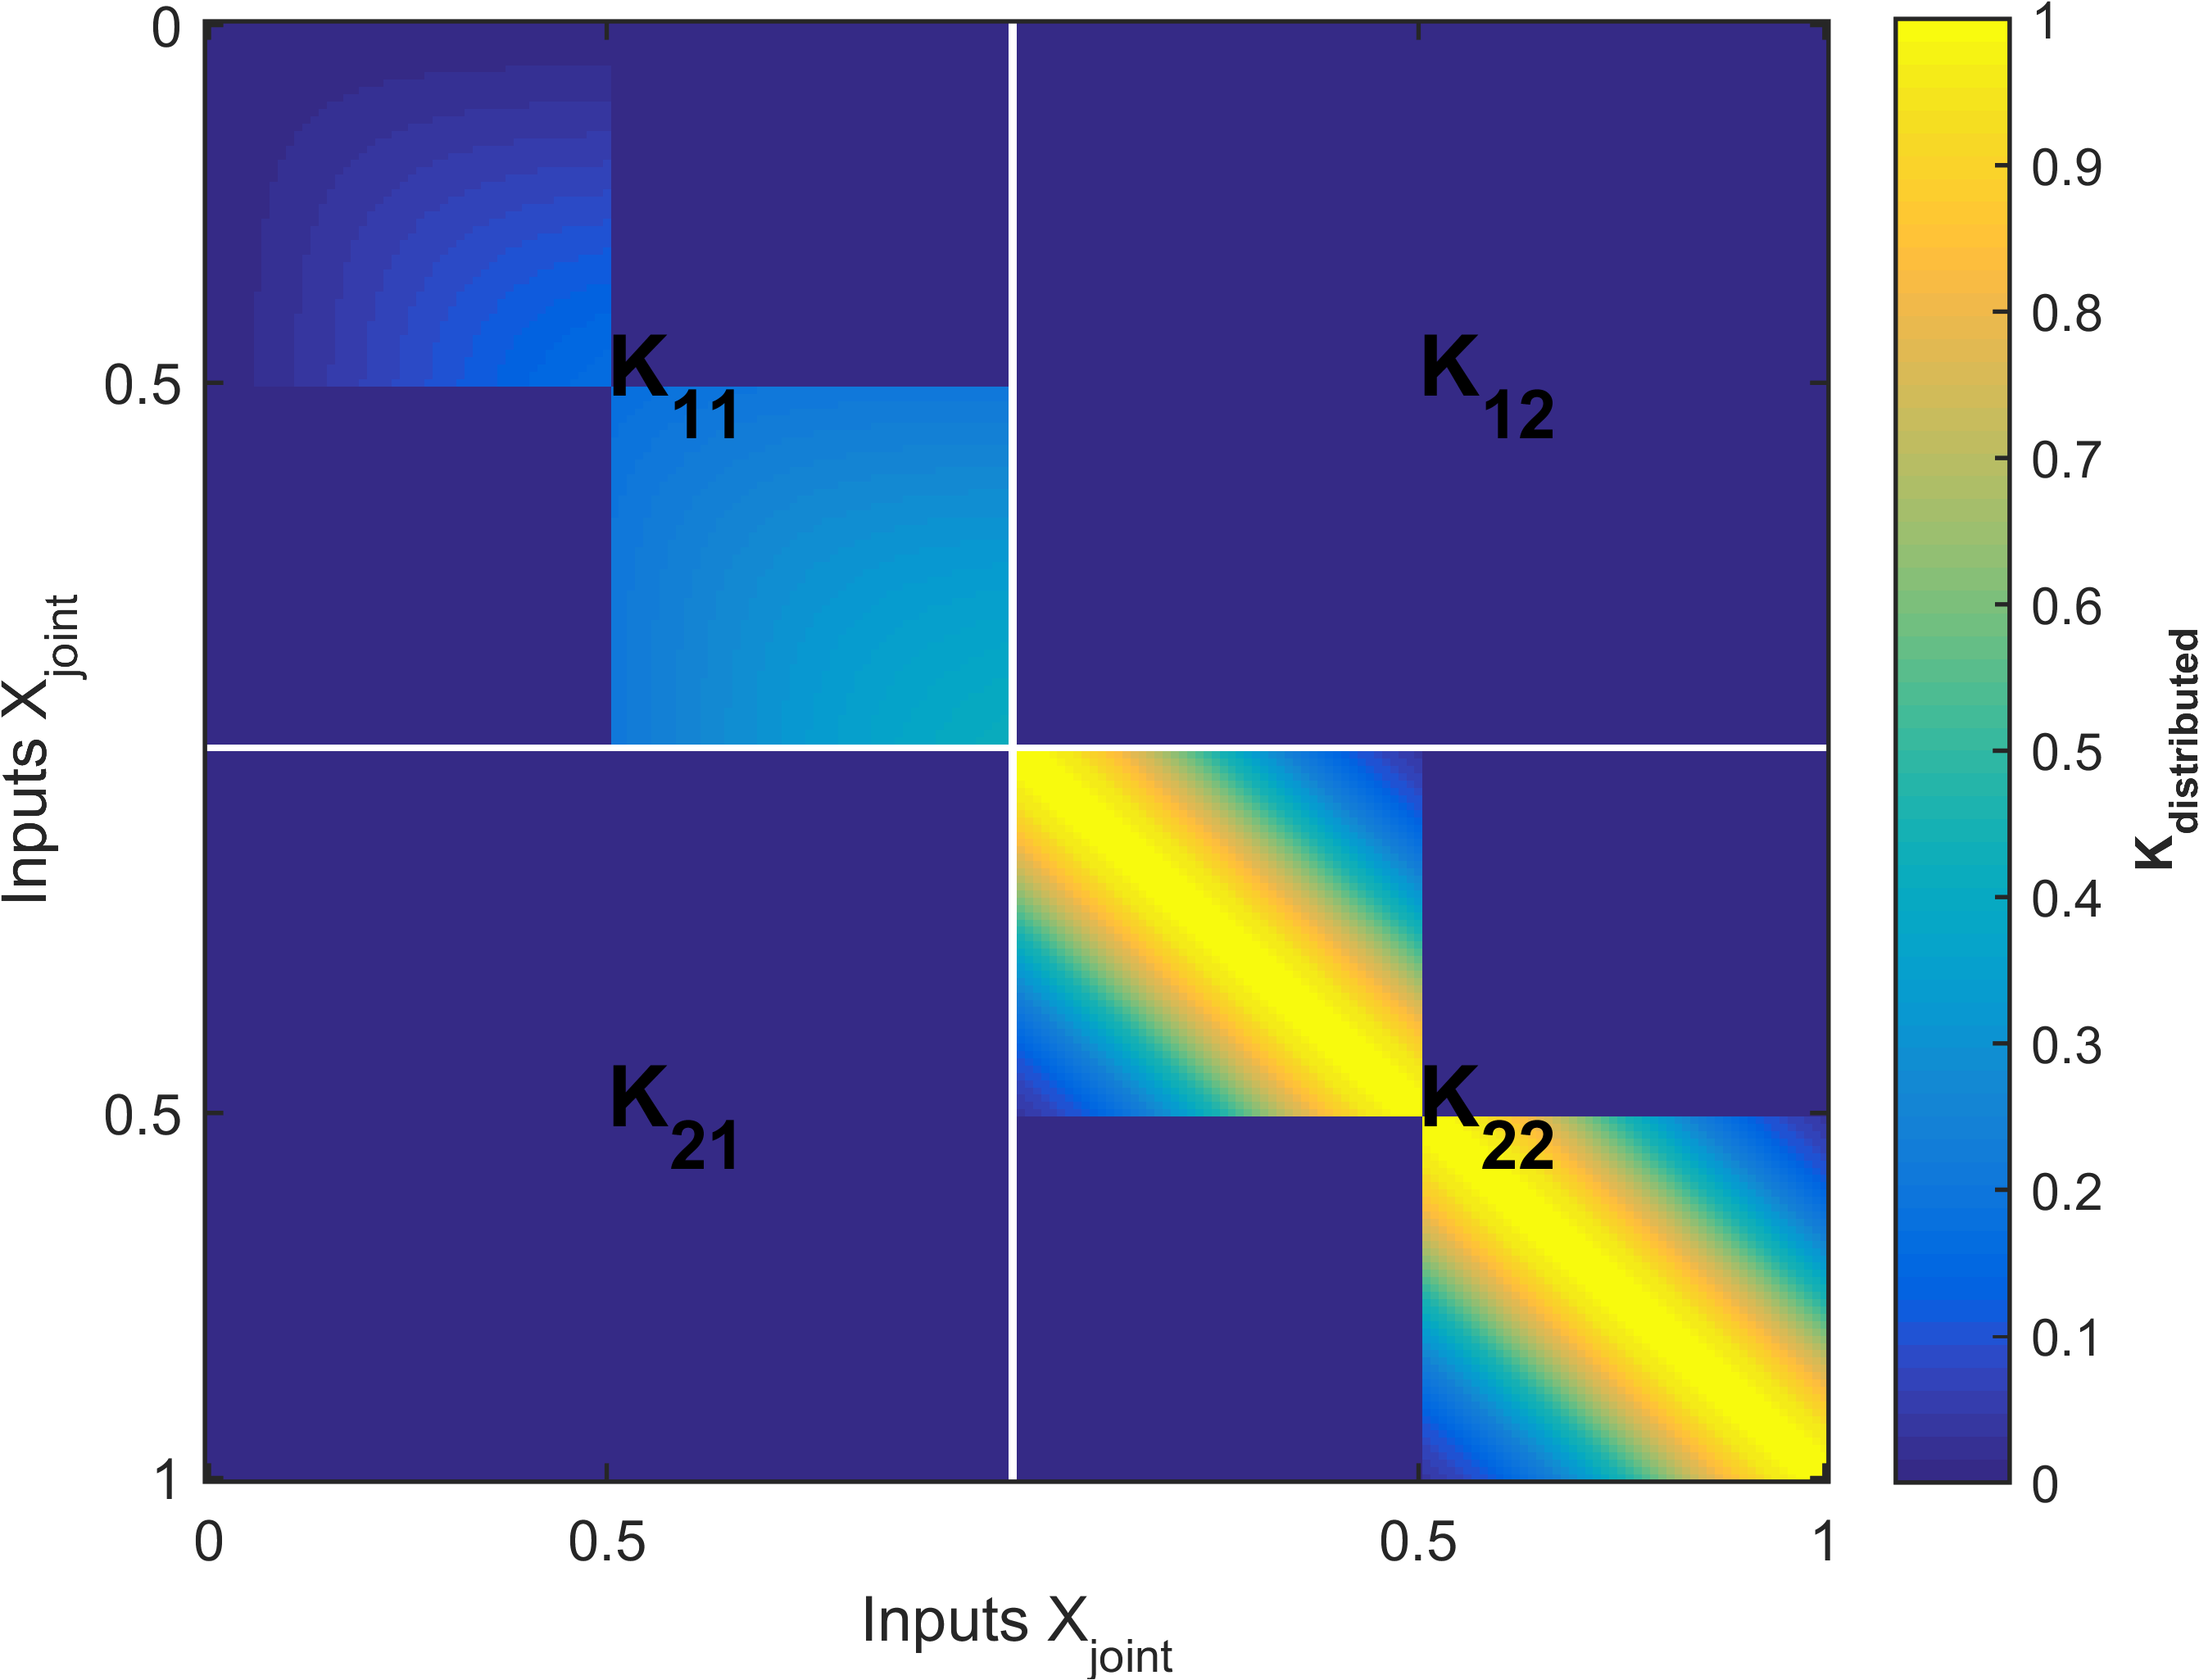
\includegraphics[width=0.45\textwidth]{images/part3/distributedJointmatrixUniform}
  \label{subfig:distributedJointmatrixUniform}}
  \caption{Approximate Gram matrix for a SE kernel using mixture of experts.}
  \label{figDGPMTGP}
\end{figure}

Equation \ref{eq:dGPNLML} describes the formulation for marginal likelihood. Due to the independence assumption, the marginal likelihood can be written as a sum of individual likelihoods and then can be optimized to find the best-fit hyperparameters. After learning the hyperparameters we can combine the predictions of local experts to give mean and variance predictions (more details in section \ref{subSecCombiningExperts}). 

\begin{align}\label{eq:dGPNLML}
    \log p(y| X, \theta) \approx \sum_{k=1}^{M} \log p_{k}(y^{(i)}| X^{(i)}, \theta)
 \end{align}

The robust Bayesian Committee Machine (rBCM) model combines the various experts using their confidence on the prediction point \cite{deisenroth2015distributed}. In such manner experts which have high confidence at the prediction points get more weight when compared to experts with low confidence. 

\begin{equation}\label{eq:meanDGP}
    m(Y_{*}) = (Cov(X_{*}))^{-2}\sum \beta_{k}\sigma_{k}^{-2}m_{k}(X_{*})
\end{equation}

\begin{equation}
    (Cov(Y_{*}))^{^-2} = \sum_{k} \beta_{k}\sigma_{k}^{-2} + (1- \sum_{k} \beta_{k})\sigma^{-2}_{**}
\end{equation}

In the above equations \(m_{k}(X_{*})\) and \(\sigma_{k}\) are the mean and covariance predictions from expert \(k\) at point \(X_{*}\). \(\sigma_{**}\) is the auto-covariance of the prior at prediction points \(X_{*}\). \(\beta_{k}\) determines the influence of experts on the final predictions \cite{DBLP:journals/corr/CaoF14} and is given as \(\beta_{k} = \frac{1}{2}(\log\sigma_{**}^{-2} - \log\sigma_{k}^{-2})\).  

\section{Experiments}\label{sec:experiments}
In the current section, we first compare the predictions of variational inference approximation, we start with a synthetic dataset where we try to learn the model over a derivative relationship. We then compare the predictions of variational joint-GP on a real-world flight-test dataset. We then empirically compare the performance of distributed Gaussian Process and Variational Inference with respect to the training time and accuracy. 

\subsection{Experiments on Theoretical Data}\label{sub:ScaleexperimentsSyntheticData}
We consider a derivative relationship between two output functions as described in equation \ref{eq:physicalRelation}. Such that 

\begin{equation}\label{eq:derivativeEquation}
   f^1 = \frac{\partial f^2}{\partial x} 
\end{equation}

Data is generated from equations \ref{eq:ScalingexperimentalSET}, a random function is drawn from GP to get \(f^{2}\) whose derivative is then calculated to generate \(f^{1}\). \(y^{1}\) and \(y^{2}\) are then calculated by adding noise according the  equations \ref{eq:ScalingexperimentalSET}. 10,000 equidistant points are generated between the locations $x \in [-1, 1]$, for both the outputs \(y^{1}\) and \(y^{2}\). Values of \(y^{2}\) are masked in the region \(x \in [0, 0.3]\), the remaining points now constitute our training dataset. 

\begin{equation}\label{eq:ScalingexperimentalSET}
    \begin{aligned}
    f^{2} & \sim  GP[0, K_{SE}(0.1, 1)] \\
\sigma_{n2} & \sim \mathcal{N}[0, 0.2] \\
\sigma_{n1} & \sim \mathcal{N}[0, 2]
    \end{aligned}
\end{equation}

\(K_{SE}(0.1, 1)\) means squared exponential kernel with length scale 0.1 and variance as 1. Since the differential relationship (\(\mathcal{L}(.)\)) is linear in nature, we use the equation \ref{eq:exactJointCovariance} to calculate the auto- and cross-covariance functions as shown in equation \ref{eq:differentialCovariances}.

\begin{equation}\label{eq:differentialCovariances}
    \begin{aligned}
Cov(f^2(x), f^2(x')) & = \theta_{amplitude}^{2}exp \left [\frac{-1}{2}\frac{d^{2}}{\theta_{lengthScale}^2} \right] \\    
Cov(f^1(x), f^2(x')) & = \theta_{amplitude}^{2}\frac{d}{\theta_{lengthScale}^2}exp\left [\frac{-1}{2}\frac{d^{2}}{\theta_{lengthScale}^2}\right] \\
Cov(f^1(x), f^1(x')) & = \theta_{amplitude}^{2}\frac{d^{2}-\theta_{lengthScale}^{2}}{\theta_{lengthScale}^{4}}exp\left [\frac{-1}{2}\frac{d^{2}}{\theta_{lengthScale}^{2}}\right]
    \end{aligned}
\end{equation}

\begin{comment}

\begin{table}[h]
\renewcommand{\arraystretch}{1.5}
\caption{Auto- and cross-covariance functions for a differential relationship.}\label{tab:differentialCovariances} \centering
\begin{tabular}{|c|c|c|}
  \hline
  Initial Covariance & \(K_{22}\) & \(\) \\
  \hline
  Cross-Covariance & \(K_{12}\) &  \(\sigma ^{2}\frac{d}{l^{2}}exp(\frac{-1}{2}\frac{d^{2}}{l^{2}})\) \\
  \hline
  Auto-covariance & \(K_{11}\) & \(\sigma ^{2}\frac{d^{2}-l^{2}}{l^{4}}exp(\frac{-1}{2}\frac{d^{2}}{l^{2}})\) \\
  \hline
\end{tabular}
\end{table}
\end{comment}


Figure \ref{fig:derivativeGP} shows comparison between an independent fit GP and a joint multi-output GP whose outputs are related through a derivative relationship described in equation \ref{eq:derivativeEquation}. For figure \ref{subfig:independentFitRelatedGP}, using variational inference algorithm, we optimize the lower bound of log-marginal likelihood for independent GP's on \(y^{1}\) and \(y^{2}\). For figure \ref{subfig:dependentFitRelatedGP}, using variational inference, we optimize the same lower bound but with a joint-covariance approach as described in section \ref{sec:varMOGP} using \(y^{1}\), \(y^{2}\) and \(\mathcal{L}(.)\). We settled on using 100 equidistant inducing points for this exercise \cite{icpram16Ankit} and have only optimized the hyperparameters to learn the model. 

Figure \ref{subfig:independentFitRelatedGP} shows the independent fit of two GP for the differential relationship while, figure \ref{subfig:dependentFitRelatedGP} shows the joint GP fit. The GP model with joint-covariance gives better prediction even in absence of data of \(y^{2}\) for \(x \in [0, 0.3]\).

\begin{figure*}[!ht]
  \centering
  \subfigure[\textbf{Independent} fit for two GP's, experiment was run on 10,000 points but only 100 data points are plotted to increase readibility. Inference is performed using variational inference algorithm and equidistant 100 inducing points. We can observe the huge difference between the real data and the predicted mean values at zone with no data.]
  {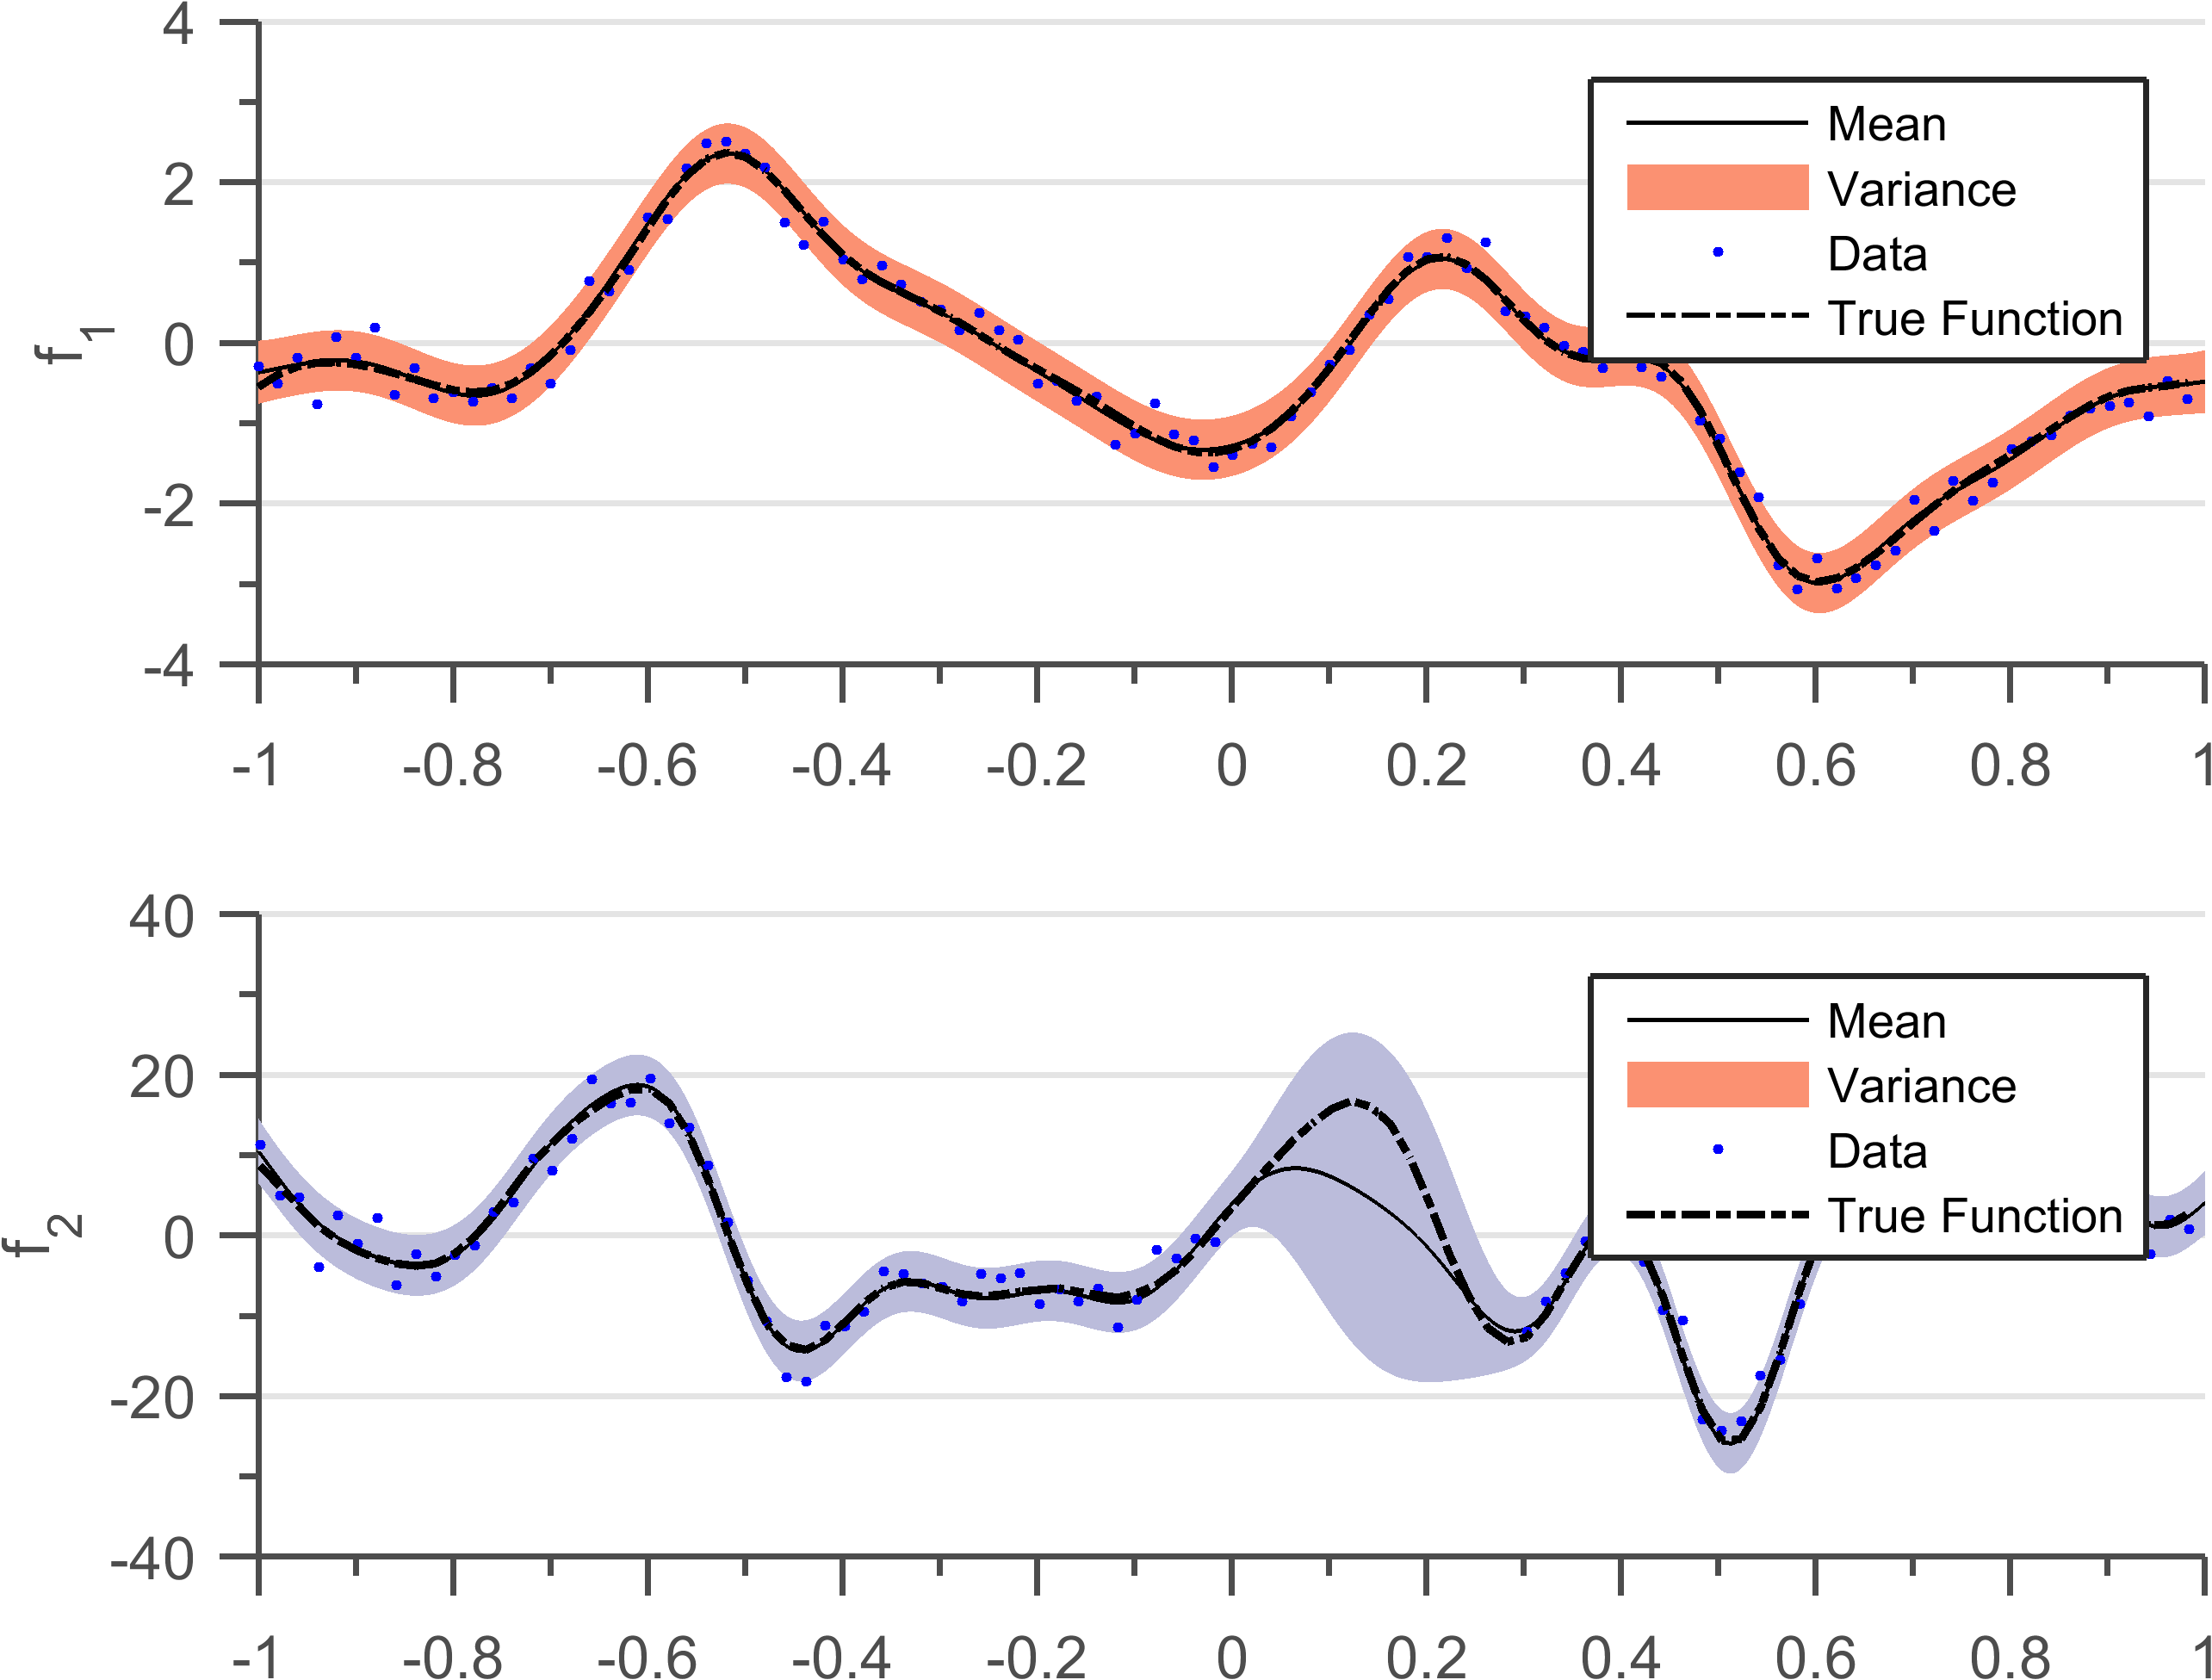
\includegraphics[width=0.45\textwidth]{images/part3/independentFitRelatedGP}
  \label{subfig:independentFitRelatedGP}}
  \quad
  \subfigure[\textbf{Joint multi-output GP's } for two outputs, experiment was run on 10,000 points but only 100 data points are plotted to increase readibility. Inference is performed using variational inference algorithm and equidistant 100 inducing points. We can observe the improved prediction between zone with no data because information is being shared between the two outputs.]
  {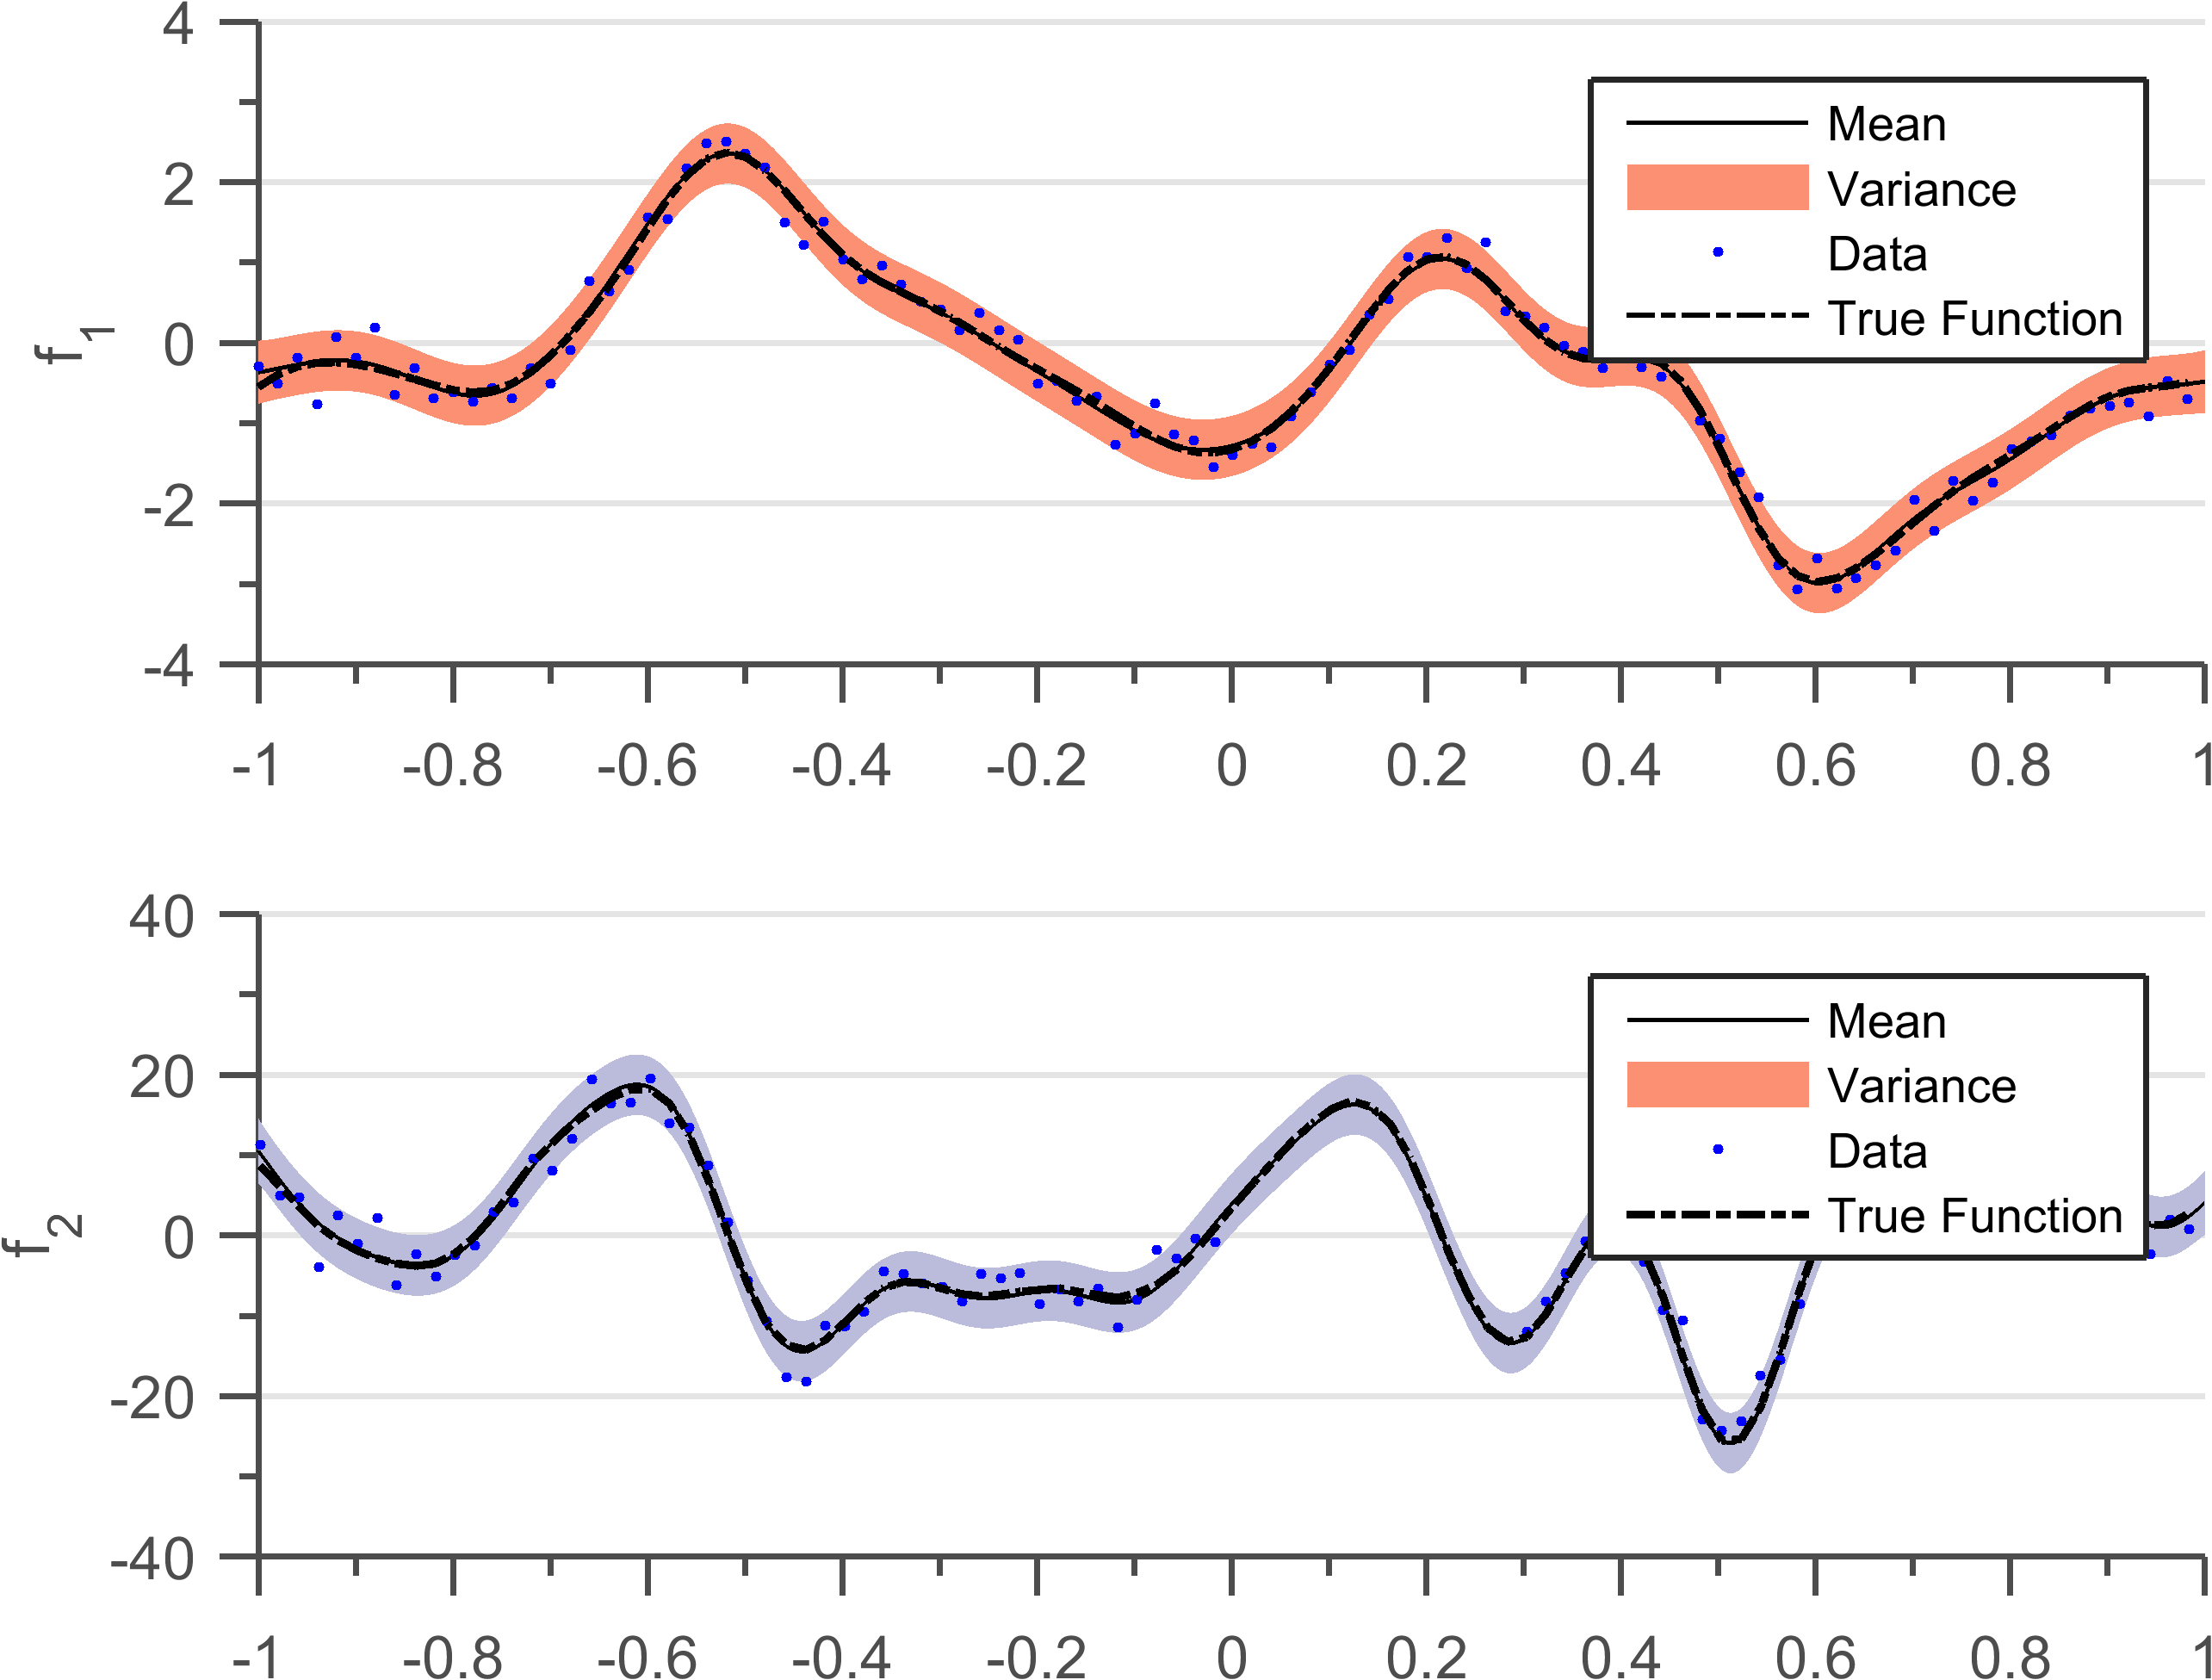
\includegraphics[width=0.45\textwidth]
  {images/part3/dependentFitRelatedGP}
  \label{subfig:dependentFitRelatedGP}}
  \caption{Experimental results for differential relationship while using variational approximation. Predicted mean is represented by solid black line. 2\(\sigma\) confidence band is represented by light red for \(f^{1}\) and light blue for \(f^{2}\). The dashed black line represents the true latent function values}\label{fig:derivativeGP}
\end{figure*}

\paragraph{\textbf{Comparison between distributed GP and variational GP}}
For the second experiment we compare the Root Mean Squared Error (RMSE) and run-times of distributed GP and Variational Inference algorithms while performing approximate inference. We progressively generate from $10^3$ to $10^5$ data-points according to the equations \ref{eq:ScalingexperimentalSET} and \ref{eq:derivativeEquation}. We separated 75\% of the data as the training set and 25\% of the data as the test set, the training and the test sets were chosen randomly. The variational inference relationship kernel as described in section \ref{sec:varMOGP} with 100 equidistant inducing points was used. We learn the optimal values of hyper-parameters for all the sets of training data. The distributed GP algorithm as described in section \ref{sec:dMOGP} was used with randomly chosen 100 points per expert. We learn the optimal values of hyper-parameters for all the sets of training data. The accuracy is plotted as RMSE values with respect to the test set. The run time is defined as time taken to calculate negative log marginal likelihood equations \ref{eq:lowerBoundMultiVarNLML} and  \ref{eq:dGPNLML}. The RMSE values are calculated for only the dependent output \(y^{1}\) and then plotted in the figure \ref{subfig:comparisonOfRunTimes}. 

In figure \ref{subfig:comparisonOfRunTimes} the time to calculate negative log-marginal likelihood with increasing number of training points is calculated. As expected the full GP takes more time when compared to variational inference or distributed GP algorithms. The Variational inference algorithm has better run-time till $\mathcal{N} \sim 10^4$ data-points, after that distributed GP takes lesser time. In figure \ref{subfig:comparisonOfRMSE}, the RMSE error with test set is compared between the variational inference and distributed GP algorithm. Here too the variational inference algorithm performs better for a lesser number of data points, but distributed GP starts performing better when we reach more than $\mathcal{N} \sim 10^4$ data points. 

\begin{figure*}[!ht]
  \centering
  \subfigure[Comparison of time to calculate negative log marginal likelihood for a Full GP, Variational inference and Distributed GP with increasing number of datapoints. We observe for datapoints greater that $10^5$ the distributed GP algorithm starts outperforming variational inference]
  {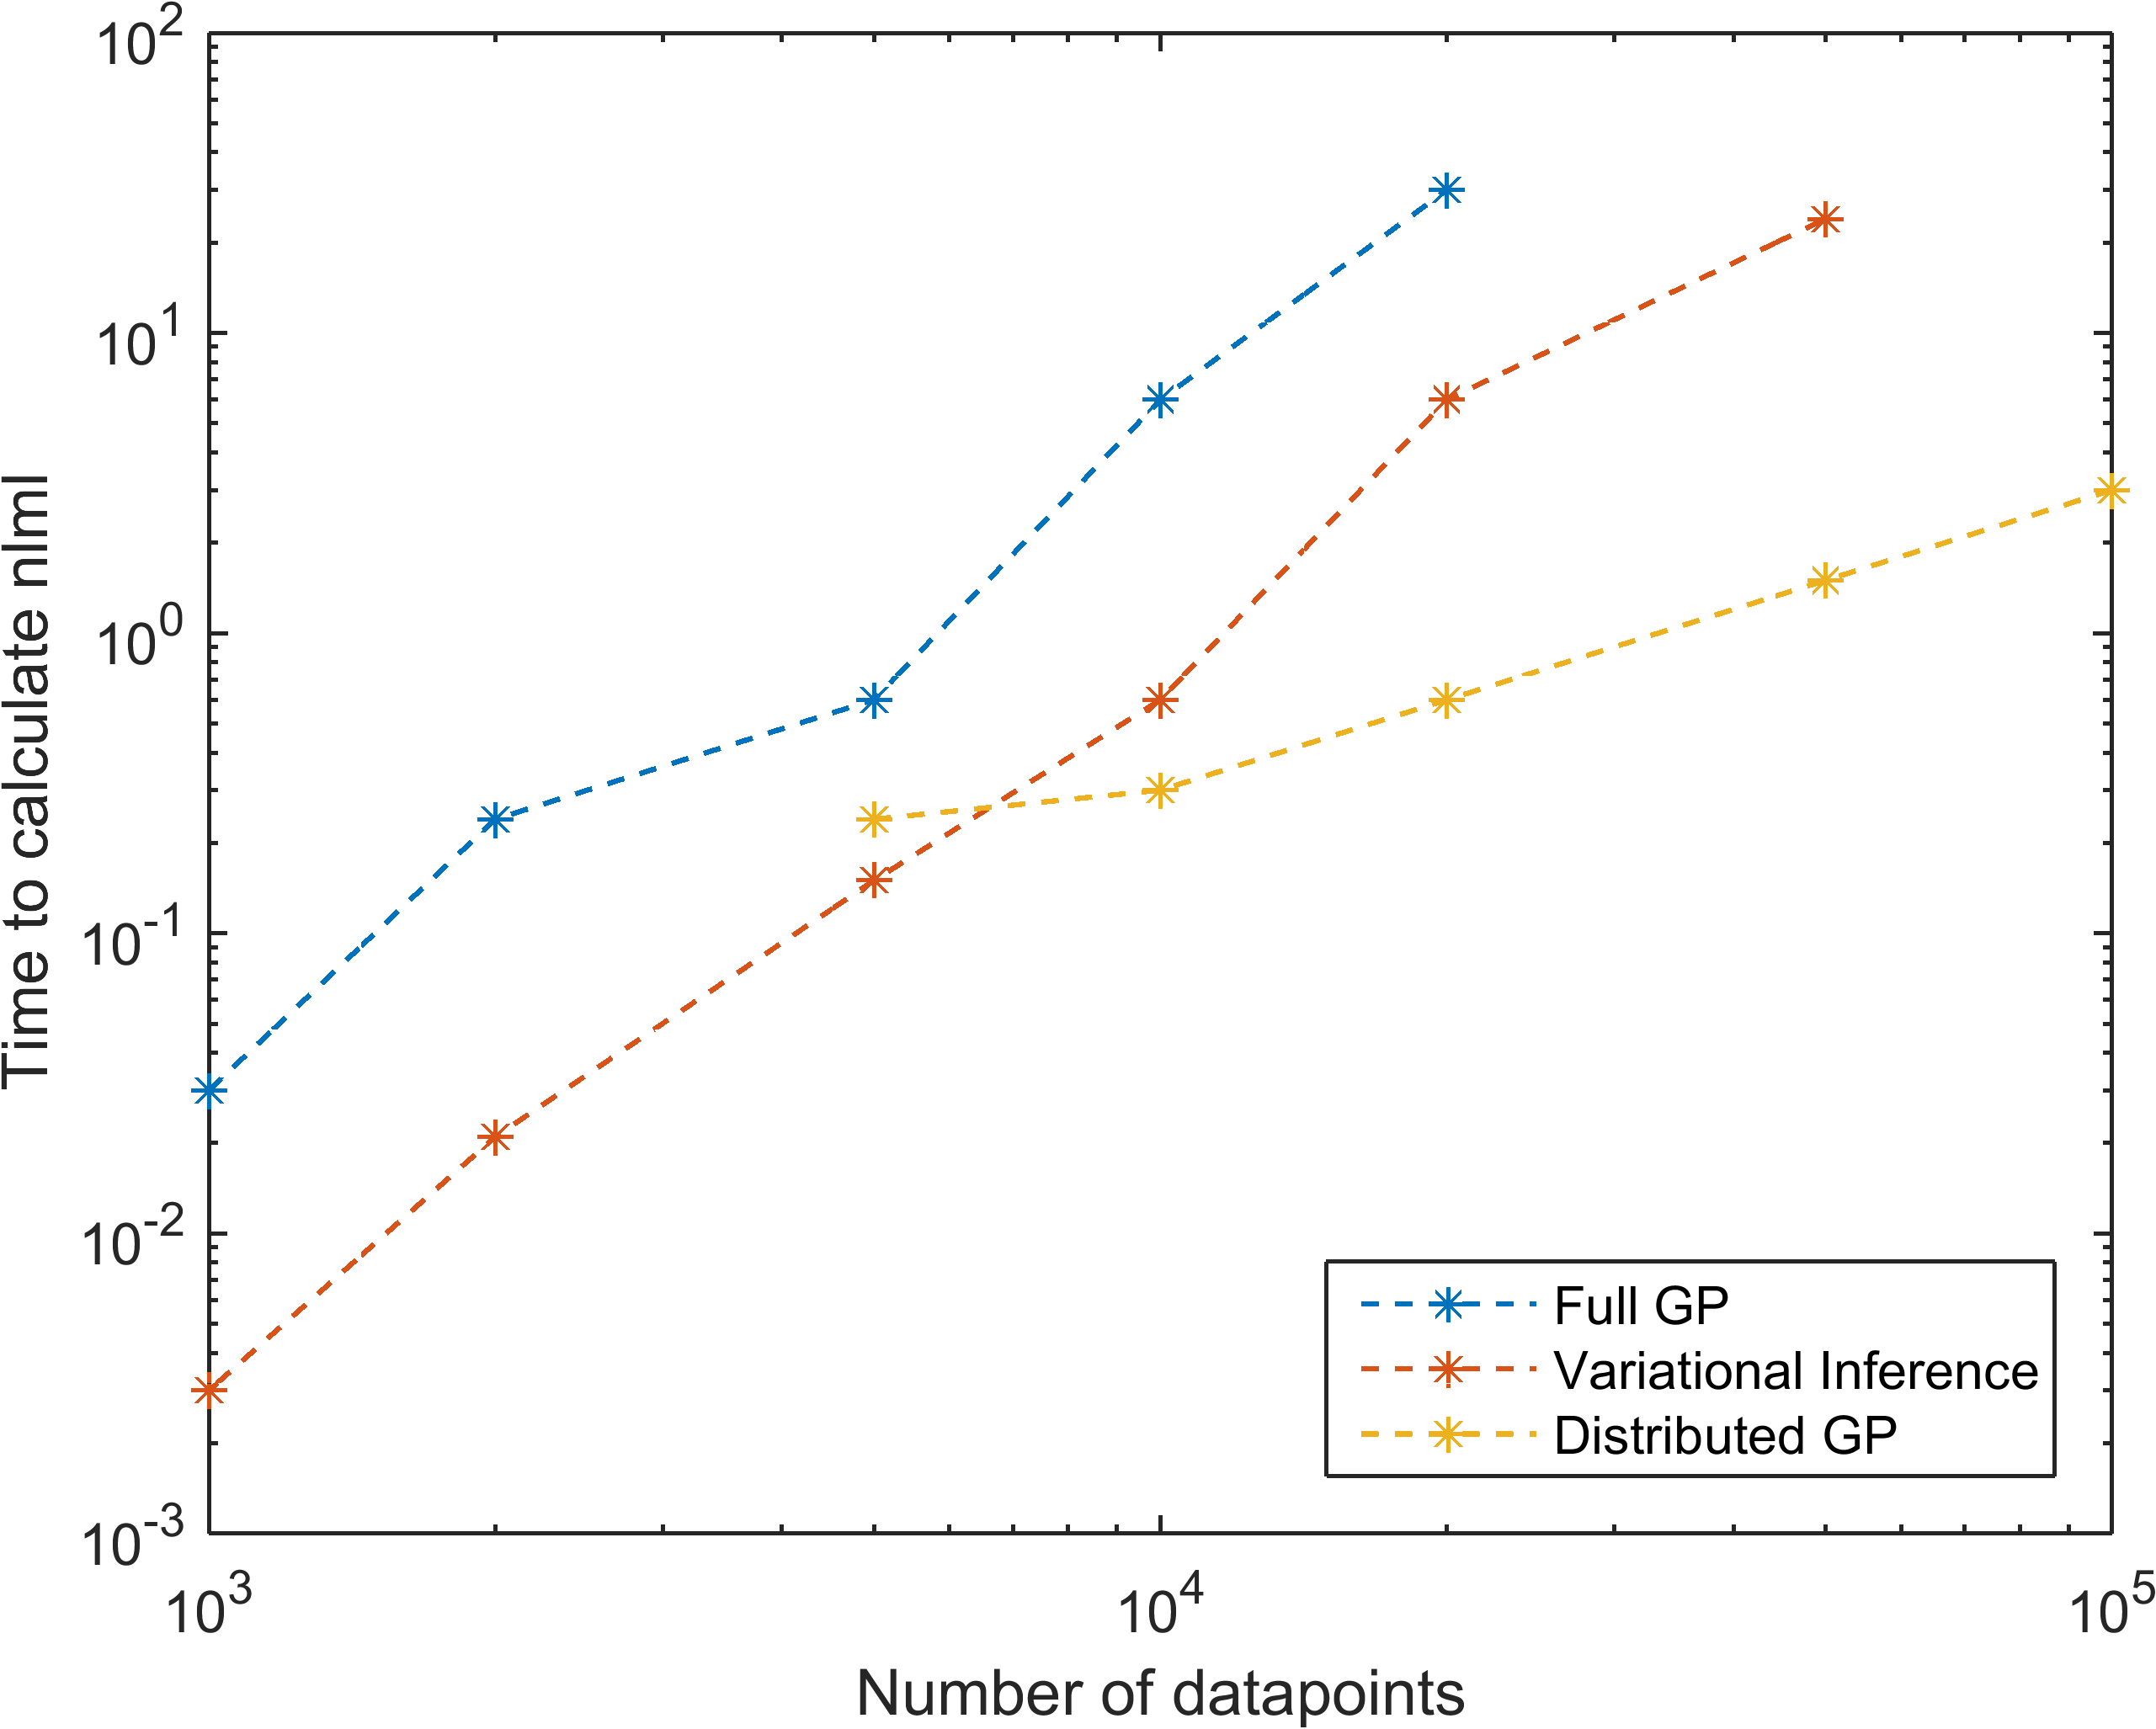
\includegraphics[width=0.45\textwidth]
  {images/part3/comparisonOfRunTimes}
  \label{subfig:comparisonOfRunTimes}}
  \quad
  \subfigure[Comparison of RMSE for variational inference and distributed GP algorithm. We observe for datapoints greater that $10^4$ the distributed GP algorithm starts outperforming variational inference.]
  {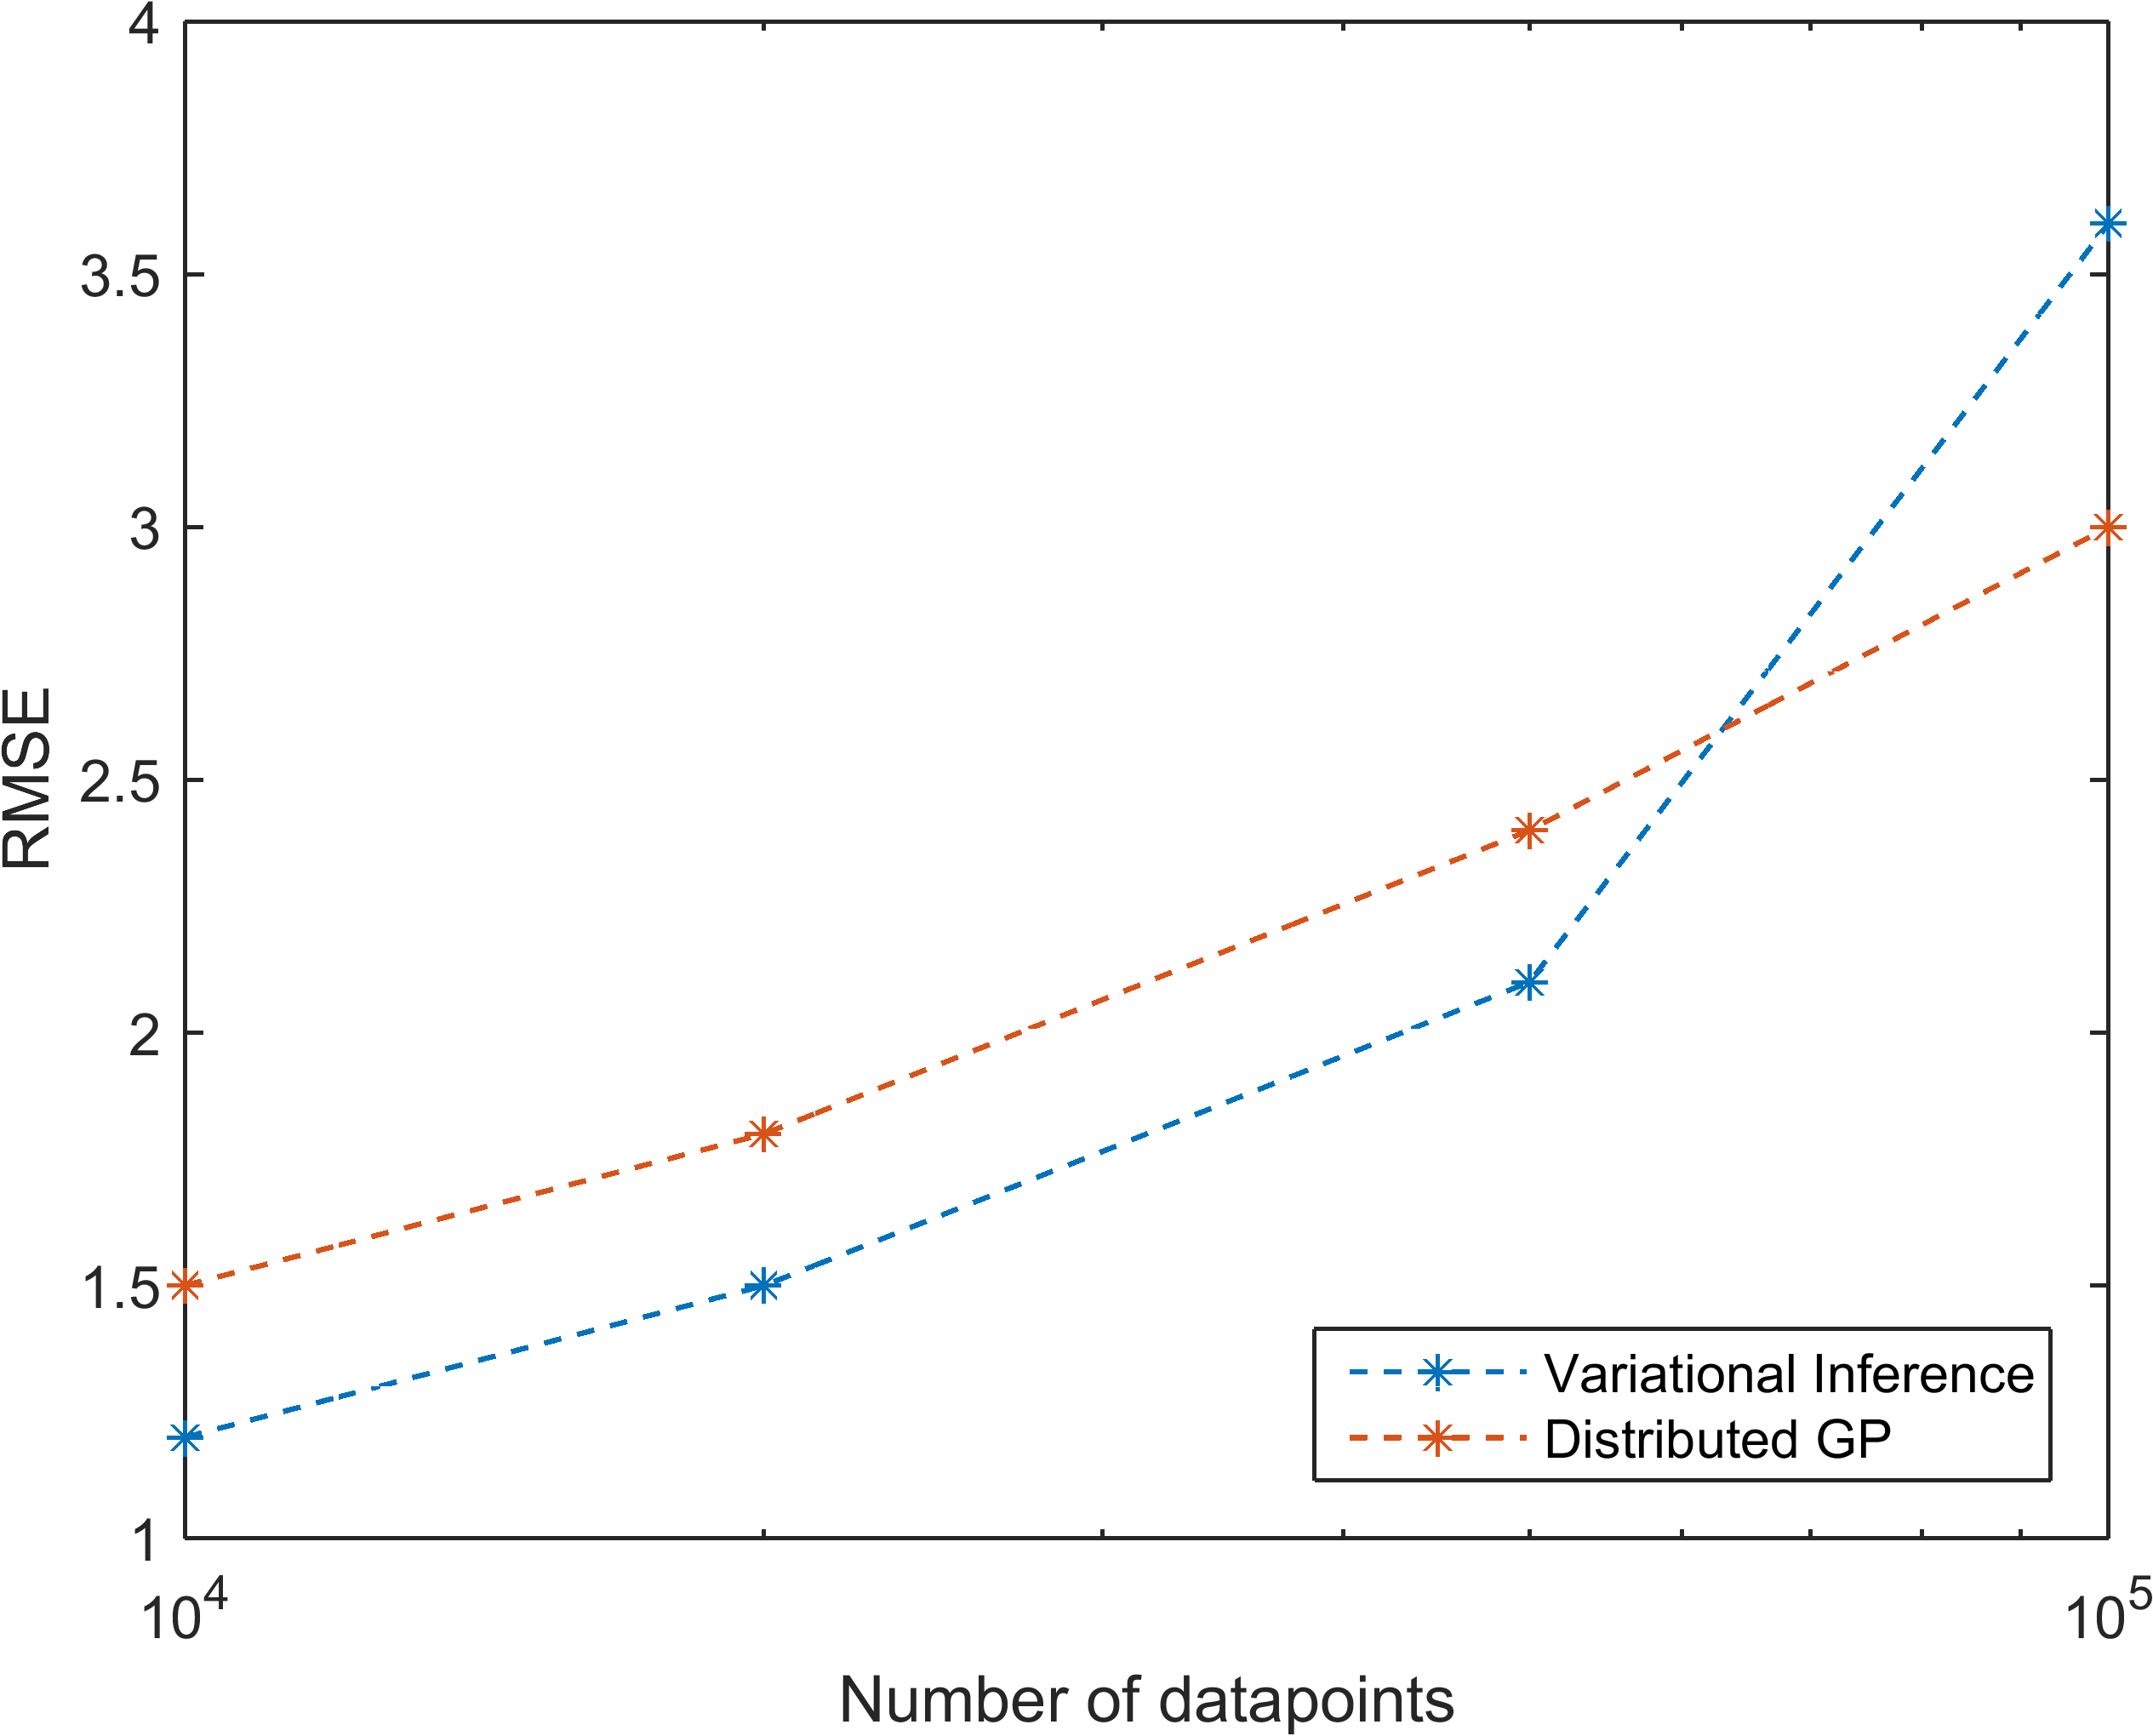
\includegraphics[width=0.45\textwidth]
  {images/part3/comparisonOfRMSE}
  \label{subfig:comparisonOfRMSE}}
  \caption{Comparison of run time and RMSE between distributed GP and Variational Inference}\label{fig:comparisonOfDGPvsVARGP}
\end{figure*}

As we keep on increasing the number of data points, for a fixed set of inducing points variational inference starts performing worse. This is because as we have already observed we need $M \sim N/10$ for good accuracy with inducing inputs approximation. If we keep the value of $M \sim N/10$ for $n \sim 10^5$ then the size of matrix $\myMatrix{K_{MM}}$ will become very big to invert efficiently. Thus even with inducing inputs approximation we have an upper limit to the possible number of meaningful GP models. One thing to note is that we have fixed the number and position of inducing points while optimizing hyperparameters for this experiment. 


While a more optimized set of inducing points will have better results, for datasets of the order $\mathcal{N} \sim 10^5$ distributed GP algorithm starts outperforming variational inference. For the case of distributed GP we have again fixed the number of points in an expert, but this does not have a significant impact on the trend on RMSE with increasing data points. 

\subsection{Experiments on Flight Test Data}\label{subsec:expFlightLoadsData}
We perform experiments on flight loads data produced during flight test phase at Airbus. Loads are measured across the wingspan using strain gauges. Shear load \(T_{z}\) and bending moment \(M_{x}\) as described in figure \ref{fig:wingLoadDiagram} are used as two outputs for this exercise. \(\eta\) or point of action of forces and angle of attack \(\alpha\) are the two inputs. The aircraft is in quasi-equilibrium in all conditions and there are no dynamic effects observed throughout this dataset. All data is normalized according to Airbus policy.

\begin{figure}
\centering
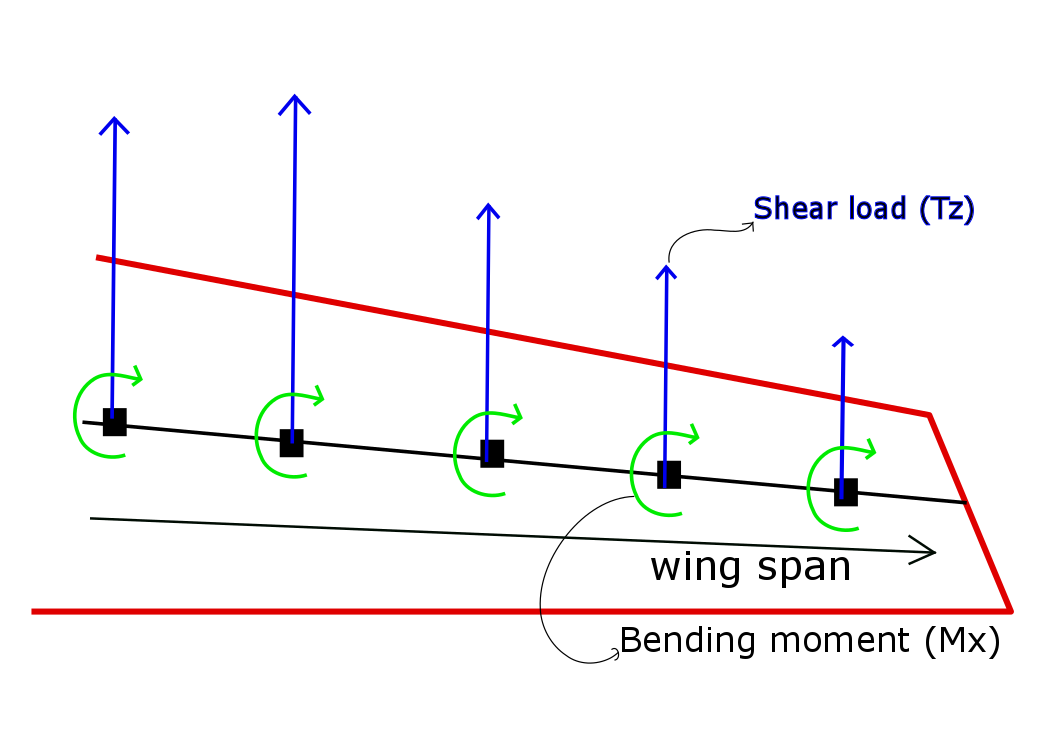
\includegraphics[width=0.5\columnwidth]{images/part3/wingLoadDiagram.png}
\caption{Wing Load Diagram}
\label{fig:wingLoadDiagram}
\end{figure}


The relation between \(T_{z}\) and \(M_{x}\) can be written as:
\begin{equation}\label{eq:relationTzMx}
\centering
M_{x}(\eta, \alpha) = \int_{\eta}^{\eta_{edge}} T_{Z}(x, \alpha)(x-\eta)dx
\end{equation}.

The equation \ref{eq:relationTzMx} is applicable for the \(\eta\) axis. Here, \(\eta_{edge}\) denotes the edge of the wingspan. The forces are measured at 5 points on the wingspan and at 8800 points on the \(\alpha\) dimension. We compare plots of relationship-imposed multi output GP and independent GP. Then we compare the measures of negative-log marginal likelihood and RMSE for varying number of inducing points.

Figure \ref{subfig:experimental_plot} shows the independent (blue shade) and joint fit (red shade) of two GP. The top figure shows \(T_{Z}\) with the variance of dependent GP plotted in red and variance of independent GP plotted in blue. The bottom figure shows plots for \(M_{X}\). Since the number of input points is less than $10^5$, we use variational inference. 100 inducing points in the input space are used to learn and plot the figure. The variance of red is smaller than that of blue showing the improvement in confidence when imposing relationships in the GP architecture. The relationship between \(T_{Z}\) and \(M_{X}\) gives rise to better confidence during the loads prediction. This added information is very useful when identifying faulty sensor data since equation \ref{eq:relationTzMx} will push data points which do not satisfy the relationship out of the tight confidence interval.

\begin{figure}[!ht]
  \centering
  \subfigure[{2\(\sigma\) confidence interval and mean of the dependent GP are represented in red shade and solid red line. 2\(\sigma\) confidence interval and mean of the independent GP are represented in blue shade and solid blue line. Experiment was run on 8800 data points Noisy data is denoted by circles only 1 \(\alpha\) step is plotted. Confidence interval improves upon adding the relationship kernel.}]
  {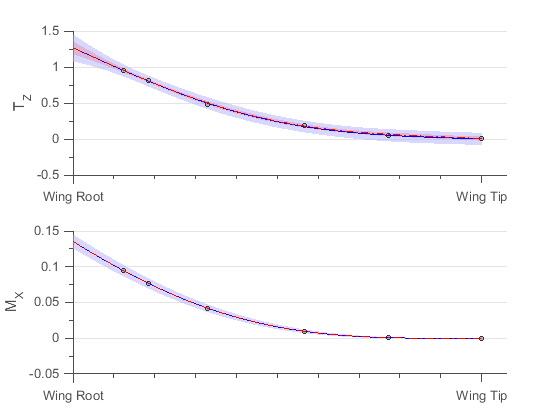
\includegraphics[width=0.45\textwidth]
  {images/part3/experimental_plots}
  \label{subfig:experimental_plot}}
  \quad
  \subfigure[{Progression of RMSE and log-likelihood upon increasing number of inducing points. Top plot shows the value of mean and variance of negative log-marginal likelihood. The bottom figure in blue shows the mean and variance of root mean squared error. 10 sets of experiments were run on 75\% of the data as training set and 25\% of the data as the test set, the training and test sets were chosen randomly.}]
  {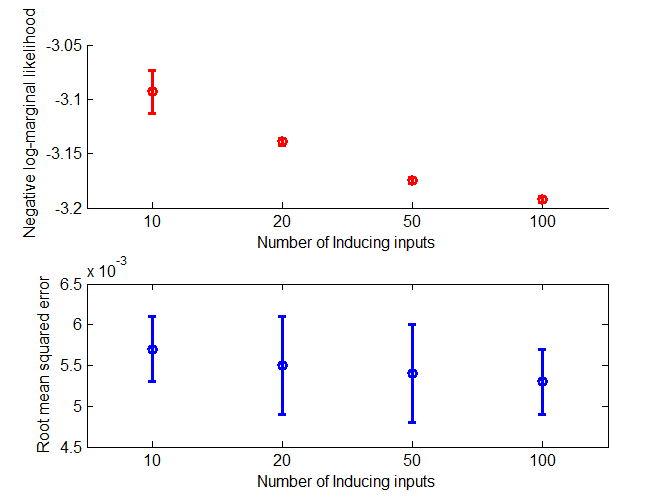
\includegraphics[width=0.45\textwidth]
  {images/part3/experimental_output_nlml_error}
  \label{subfig:experimental_nlml_error}}
  
\caption{Experimental results for aircraft flight loads}
  \label{fig:expFlightLoadsRelationship}
\end{figure}

Figure \ref{subfig:experimental_nlml_error} shows improvement in the negative log-marginal likelihood and RMSE plots upon increasing number of inducing points. 10 sets of experiments were run on 75\% of the data as training set and 25\% of the data as the test set, the training and the test sets were chosen randomly. We learn the optimal values of hyper-parameters and inducing points for all the 10 sets of experiments of training data. Finally, RMSE values are evaluated with respect to the test set and negative log-marginal likelihood are evaluated for each learned model. The RMSE and log-likelihood improve upon increasing the number of inducing points. 

\paragraph{Cost saving in MDO}
By enabling relationships in building models we can save significant costs while performing MDO. Earlier works have reduced the cost of optimization by incorporating Gradient Enhanced Kriging into the optimization process \cite{liem2015surrogate}, a similar cost saving can be obtained by using the proposed methods. Suppose we are designing a part of an aircraft by performing optimization over a fluid-structure interaction loop. The fluid part is being solved by a costly CFD code, while the structural part is being solved by a cheap CSM code. The CFD code results in $pressures$ on the aerodynamic mesh, while the CSM part results in $deformations$ of the structural mesh. If we can leverage the relationship between pressure and deformation ($\int pressures = Stiffness \times deformation$) then we can effectively reduce the number of required runs. These type of cost savings can be made in several MDO problems. 


\section{Summary and discussion}
The current chapter demonstrates how to incorporate physical laws into multi-output GP regression framework and then eventually how to scale the framework to a large number of data points. Section \ref{subsecLinearOperators} demonstrates how to enforce physical laws, which are in the form of linear operators. Whereas section \ref{subsecNonLinearOperators} demonstrates how to encode physical laws, which are in the form of non-linear operators. The improved accuracy of the model is then demonstrated both on a toy dataset and a dataset of real flight-test (section \ref{sec:results}). 

Section \ref{sec:sparseGPRegression} demonstrates how to scale the MTGP to large number of outputs, both using a variational approximation (section \ref{sec:varMOGP}) and a distributed GP approximation (section \ref{sec:dMOGP}). We then demonstrate the scalability on a toy dataset and a dataset from flight test and compare the accuracy of distributed GP and variational inference on the toy-dataset. 

Several future paths can be explored by leveraging this kind of relationship enabled MTGP's. Using a quadratic relationship enabled MTGP we can indirectly add inequality constraints. Leveraging the information of prior relationships can greatly reducs the cost of performing MDO. Finally, by enforcing physical laws of the system we can automatically identify faulty sensors. All these are inetresting paths and should be explored further. 

%%% Local Variables: 
%%% mode: latex
%%% TeX-master: "isae-report-template"
%%% End: 

